\documentclass[a4paper,12pt]{article}
\usepackage[ngerman]{babel}
% \usepackage[ngerman]{babel}
\usepackage[utf8]{inputenc}
\usepackage[T1]{fontenc}
\usepackage{lmodern}
\usepackage{titling}
\usepackage{geometry}
\geometry{left=3cm, right=3cm, top=2cm, bottom=3cm}
\usepackage{setspace}
\onehalfspacing

\usepackage{ifthen}

\usepackage{graphicx}
% \usepackage{pstricks}
% \usepackage{relsize}
% \usepackage[decimalsymbol=comma,exponent-product = \cdot, per=frac]{siunitx}
% \sisetup{range-phrase=\,bis\,}

\usepackage{xargs}
\usepackage{calc}
\usepackage{amsmath}
\usepackage{amsfonts}
\usepackage{mathtools}
\usepackage{amssymb}

\usepackage{cancel}
\usepackage{trfsigns}
\usepackage{array}
\usepackage{enumerate}
\usepackage{enumitem}

\usepackage{caption}
\usepackage{subcaption}

\usepackage{multicol}

\usepackage{pdflscape}
\usepackage[table]{xcolor}

\usepackage{float}

%%%%%%%%%%%%%%%%%%%%%%%%%%%%%%%%%%%%%%%%%%%%%%%%%%%%%%%%%%%%%%%%%%%%%%%%%%%%%%%%
\newboolean{WITHPSTRICKS}
\setboolean{WITHPSTRICKS}{false}


%%%%%%%%%%%%%%%%%%%%%%%%%%%%%%%%%%%%%%%%%%%%%%%%%%%%%%%%%%%%%%%%%%%%%%%%%%%%%%%%%
\newboolean{mitLoes}
\setboolean{mitLoes}{false}
\setboolean{mitLoes}{true}

%%%%%%%%%%%%%%%%%%%%%%%%%%%%%%%%%%%%%%%%%%%%%%%%%%%%%%%%%%%%%%%%%%%%%%%%%%%%%%%%
%\setboolean{mitErg}{false}
%\setboolean{mitErg}{true}

%\setboolean{WITHPSTRICKS}{false}
\setboolean{WITHPSTRICKS}{true}


\usepackage{tikz}
\usetikzlibrary{arrows,automata,backgrounds,calendar,decorations.pathmorphing,fadings,shadings,calc,intersections}
\usetikzlibrary{decorations.pathreplacing}
\usetikzlibrary{decorations.shapes}
\usetikzlibrary{decorations.footprints}
\usetikzlibrary{decorations.text}
\usetikzlibrary{positioning}
\usetikzlibrary{through}

\ifthenelse{\boolean{WITHPSTRICKS}}{%
\usepackage{auto-pst-pdf}
\usepackage{pstricks,pst-plot,pst-text}
}{}

\usepackage{pgfplots}

%%%%%%%%%%%%%%%%%%%%%%%%%%%%%%%%%%%%%%%%%%%%%%%%%%%%%%%%%%%%%%%%%%%%%%%%%%%%%%%%
\usepackage{mbdefAufgaben}

%%%%%%%%%%%%%%%%%%%%%%%%%%%%%%%%%%%%%%%%%%%%%%%%%%%%%%%%%%%%%%%%%%%%%%%%%%%%%%%%
\newboolean{mitErg}
\setboolean{mitErg}{false}

%%%%%%%%%%%%%%%%%%%%%%%%%%%%%%%%%%%%%%%%%%%%%%%%%%%%%%%%%%%%%%%%%%%%%%%%%%%%%%%%
\newcounter{Aufg}
\setcounter{Aufg}{0}
\newcounter{Blatt}
\setcounter{Blatt}{\BLATT}

%%%%%%%%%%%%%%%%%%%%%%%%%%%%%%%%%%%%%%%%%%%%%%%%%%%%%%%%%%%%%%%%%%%%%%%%%%%%%%%%
\usepackage{KopfEnglish}

% Seitenraender
\textwidth = 285mm
\textheight = 180mm
\leftmargin 5mm
\oddsidemargin = -20mm
\evensidemargin = -20mm
\topmargin = -25mm
\parindent 0cm
\columnsep 2cm

% % % Aufgabenstellung
% % % Schwierungkeitsgrad mit "e" , "f" oder "v" angeben
% % % "e" Einführung   
% % % "f" Festigung
% % % "v" Vertiefung  

\newcommand{\Aufgabe}[3][]{
\stepcounter{Aufg}
\subsubsection*{Aufgabe 
\arabic{Blatt}.\arabic{Aufg}\ifthenelse{\equal{#1}{e}}{}{\ifthenelse{\equal{#1}{f}}{
$\!\!{}^\star$}{\ifthenelse{\equal{#1}{v}}{$^{\star\star}$}{}}}{: #2}}
{#3}
}
% % % Ergebnisse jeweils am Ende des Aufgabenblattes Anzeigen
\newcommand{\Ergebnisse}{}
\makeatletter
\newcommand{\Ergebnis}[1]{
	\g@addto@macro{\Ergebnisse}{#1}
}
\makeatother
\makeatletter
\newcommand{\ErgebnisC}[2]{
\@ifundefined{c@#1}
{\newcounter{#1}}
{}
\setcounter{#1}{\theAufg}

\ifthenelse{\boolean{mitErg}}{	\g@addto@macro{\Ergebnisse}{\subsubsection*{Ergebnisse zu Aufgabe \arabic{Blatt}.\arabic{#1}:}
}%
	\g@addto@macro{\Ergebnisse}{#2}}{}
}
\makeatother


% % % Lösungen
\newcommand{\Loesung}[1]{
	\ifthenelse{\boolean{mitLoes}}
	{\subsubsection*{Lösung \arabic{Blatt}.\arabic{Aufg}:}
		#1}
	{}
}
% % % % % % % % % % % % % % % % % % % % % % % % % % % % % % % % % % % % % % % % % % % % % % % % % % % % % %
% % % % % % % % % % % % % % % % % % % % % % % % % % % % % % % % % % % % % % % % % % % % % % % % % % % % % %
% % % % % % % % % % % % % % % % % % % % % % % % % % % % % % % % % % % % % % % % % % % % % % % % % % % % % %
\begin{document}
\begin{twocolumn}
% % % % % % % % % % % % % % % % % % % % % % % % % % %

%%%%%%%%%%%%%%%%%%%%%%%%%%%%%%%%%%%%%%%%%%%%%%%%%%%%%%%%%%%%%%%%%%%%%%%%%%%%%%%%
% Set the TITLE of the sheet here:
%\uebheader{\Kurs}{\arabic{Blatt}}{\Trimester\,\Jahr}{\TOPIC}
%\uebheader{\Kurs}{\arabic{Blatt}}{\Trimester\,\Jahr}{\TOPIC}
\uebheader{\Kurs}{\arabic{Blatt}}{\Trimester\,\Jahr}{\TOPIC}
\ruleBig

\thispagestyle{empty} 
% Logo
\begin{center}
    \vspace*{2cm}
    
\includegraphics[width=0.3\textwidth]{HSU_RGB.eps} % <- Logo-Dateiname hier einfügen
\end{center}

% Titel
\begin{center}
    \vspace{1cm}
    {\LARGE \textbf{Aufgabensammlung}}\\
    \vspace{0.5cm}
    {\LARGE \textbf{Mathematik III/B}} \\
    \vspace{0.5cm}
    {\large f\"ur WI/ET} \\
\end{center}


% Universität
\vfill
\begin{center}
    {\large Prof. Dr. Thomas Carraro} \\
    {\large Fr\"uhjahrstrimester 2025}
\end{center}

\newpage
\thispagestyle{empty}
\mbox{}
\newpage
% Inhaltsverzeichnis
\tableofcontents
\newpage
\thispagestyle{empty}
\mbox{}
\newpage

%\setboolean{mitErg}{false}
\setboolean{mitErg}{true}


%%%%%%%%%%%%%%%%%%%%%%%%%%%%%%%%%%%%%%%%%%%%%%%%%%%%%%%%%%%%%%%%%%%%%%%%%%%%%%%%
% Set the INTRODUCTION section of the sheet here:
% \input{introduction.tex}
\renewcommand{\d }{\mathrm{d}}
%\ruleBig
\setcounter{page}{1}

\section*{Gew\"ohnliche Differentialgleichungen}
\addcontentsline{toc}{section}{Gew\"ohnliche Differentialgleichungen}
Eine gew\"ohnliche Differentialgleichung (Dgl.) ist eine Gleichung, die aus einer unbekannten Funktion $y(x)$ und ihren Ableitungen $y'(x)$, $y''(x)$,..., $y^m(x)$ besteht, wobei die Funktion $y$ nur von einer Variablen $x$ abh\"angt und nur nach dieser abgeleitet wird. Es wird zwischen einer \textbf{impliziten} Darstellung der Differentialgleichung \textbf{$n$-ter Ordnung}
$$
F(x, y'(x), y''(x),..., y^n(x)) =0
$$
und einer \textbf{expliziten} Darstellung der Differentialgleichung $n$-ter Ordnung
$$
y^n(x) = f(x, y'(x), y''(x),..., y^{n-1}(x)) 
$$
unterschieden. Die Differentialgleichung hei\ss t \textbf{autonom}, wenn $F$ bzw. $f$ nicht explizit von $x$ abh\"angt. \\

\noindent
Eine Differentialgleichung ist \textbf{linear}, wenn sie die Form
$$
a_n(x)\, y^{(n)} + a_{n-1}(x)\, y^{(n-1)} + \dots + a_1(x)\, y' + a_0(x)\, y = f(x)
$$
besitzt, wobei $a_n(x)$ \textbf{variable Koeffizienten} sind. H\"angen die Koeffizienten nicht von $x$ ab, so handelt es sich um \textbf{konstante Koeffizienten}.
Man spricht von einer \textbf{homogene} Dgl., wenn $f(x)$=0 ist. Gilt $f(x) \neq 0$, dann handelt es sich um eine \textbf{inhomogene} Differentialgleichung.\\

\noindent
Eine Differentialgleichung zusammen mit einer Anfangsbedingung hei\ss t \textbf{Anfangswertproblem} (AWP) und haben z.B. die Form
$$
y'(x)=f(x,y(x)), \,  y(x_0) = y_0,
$$
wobei $x_0$ und $y_0$ gegebene Werte sind.\\

\noindent
Beispiele f\"ur \textbf{nichtlineare} Differentialgleichungen sind:
\begin{align*}
y' &= y^2, \\
y'' +y \, y' &= 0,\\
y' &= \sin(y).
\end{align*}

\subsection*{Explizite Differentialgleichung 1. Ordnung}
Eine explizite Dgl. 1. Ordnung besitzt die Form
$$
\dfrac{\mathrm{d}y}{\mathrm{d}x}:= y' = f(x,y),
$$
wobei $f$ im Allgemeinen eine nichtlineare Funktion ist. \\
\noindent
\textbf{Typ A: Differentialgleichungen mit getrennten Ver\"anderlichen}
Liegt die Differentialgleichung in der Form
$$
y' =f(x)\cdot g(y)
$$
vor, wobei $f$ und $g$ stetige Funktionen sind, so kann das L\"osungeverfahren der \textbf{Trennung der Ver\"anderlichen} (TdV) angewendet werden. Die L\"osung ist dann gegeben durch
$$
\int \dfrac{\mathrm{d}y}{g(y)} = \int f(x) \, \mathrm{d}x +C.
$$

\textbf{Typ B: Homogene Differentialgleichung}


\textbf{Typ C:$y' = f(ax+by+c)$}

\textbf{Typ D: Lineare Differentialgleichung 1. Ordnung}

\textbf{Typ E: Bernoulli-Differentialgleichung}

\textbf{Typ F: Riccati-Differentialgleichung}

\subsection*{Lineare Differentialgleichung h\"oherer Ordnung}

\subsubsection*{Homogene lineare Differentialgleichung}

\subsubsection*{Inhomogene lineare Differentialgleichung}
\newpage
\section*{Aufgaben zu gew\"ohnlichen Differentialgleichungen}
\addcontentsline{toc}{section}{Aufgaben zu gew\"ohnlichen Differentialgleichungen}
%1
\Aufgabe[e]{Anfangswertproblem}
{
Gegeben ist die Dgl.
$$
y'(x) = \dfrac{1}{y\sqrt{x}}, \, x>0, \, y \neq 0
$$
mit der allgemeinen L\"osung
$$
y(x) = \pm \sqrt{4\sqrt{x}+C}, \, C\geq 0.
$$
\begin{abc}
\item Geben Sie, falls m\"oglich, die L\"osung der Dgl. an, die die Anfangswertbedingung $y(1)=3$ erf\"ullt.
\item Geben Sie, falls m\"oglich, die L\"osung der Dgl. an, die die Anfangswertbedingung $y(1)=-4$ erf\"ullt.
\item Geben Sie, falls m\"oglich, die L\"osung der Dgl. an, die die Anfangswertbedingung $y(-1)=3$ erf\"ullt.
\end{abc}
}

\Loesung{
\begin{abc}
\item Die Konstante $C$ muss so bestimmt werden, dass die allgemeine L\"osung $y(x) = \pm \sqrt{4\sqrt{x}+C}$ die Anfangsbedingung $y(1)=3$ erf\"ullt:
$$
3 = \pm \sqrt{4\sqrt{1}+C} \Rightarrow 3 = + \sqrt{4+C} \Rightarrow C=5.
$$
Die Anfangsbedingung legt also sowohl das Vorzeichen, als auch die Konstante fest. Die spezielle L\"osung des AWP ist also
$$
y(x) = \sqrt{4\sqrt{x}+5}, \, x\geq 0.
$$
\item Analog zu Aufgabenteil a):
$$
-4 = \pm \sqrt{4\sqrt{1}+C} \Rightarrow -4 = - \sqrt{4+C} \Rightarrow C=12.
$$
Es ergibt sich die spezielle L\"osung 
$$
y(x) = -\sqrt{4\sqrt{x}+12}, \, x\geq 0.
$$
\item Es gibt keine L\"osung, da die Dgl. nicht bei $x=-1$ definiert ist
\end{abc}
}


\ErgebnisC{gewdgl_Anfangswertproblem}{
\begin{abc}
\item $y(x) = \sqrt{4\sqrt{x}+5}, \, x\geq 0$
\item $y(x) = -\sqrt{4\sqrt{x}+12}, \, x\geq 0$
\item keine L\"osung, da Dgl. nicht bei $x=-1$ definiert ist
\end{abc}
}


\ifthenelse{\boolean{mitLoes}}{\ruleBig \cleardoublepage}{}
%2
\input{../GewDgln/gewdgl_Begriff_Dgl.tex}
\ifthenelse{\boolean{mitLoes}}{\ruleBig \cleardoublepage}{}
%3
\Aufgabe[e]{Definitionsbereich der Lösung einer Dgl.}
{
\begin{abc}
\item Bestimmen Sie die allgemeine Lösung der Differentialgleichung 
\[
y'(x)=2\,x\,y^2 
\]
und die spezielle Lösung für den Anfangswert \ $y(0)=4$\ .

Wie groß ist der maximale Definitionsbereich dieser Lösung\thinspace ?\\
\item Bestimmen Sie die allgemeine Lösung der Differentialgleichung
	\[
	\cos(x)\cdot y'(x) = \sin(x)\cdot y(x).
\]
\end{abc}
}

\Loesung{
\begin{abc}
\item Die Dgl. ist vom trennbaren Typ 
\[
	\int\frac{\text dy}{y^2} = \int2x\ \text dx \,\Rightarrow\, \frac{y^{-1}}{-1} = x^2+ C \quad\vee\quad y=0
\]
und hat die allgemeine Lösung 
\[
y(x)=\frac{-1}{x^2+C}\;\;,\;\;\;\;C\in\mathbb{R}\;\quad \text{bzw. } y=0
\]

Der Anfangswert \ $y(0)=4$ \ ergibt mit \ $C=-\frac{1}{4}$ \ die Lösung 
\[
y_{\text{AWP}}(x)=\frac{-1}{x^{2}-\frac{1}{4}}\ . 
\]
Die Lösung ist nur im Bereich \ $\frac{-1}{2}<x<\frac{1}{2}$ \ definiert und hat an den Rändern bei \ $x=\pm \frac{1}{2}$ \
Polstellen.

\item L\"osen der homogenen linearen Dgl. \ 
$$
\cos(x)\cdot y'(x) = \sin(x)\cdot y(x)$$ 
durch Trennung der Veränderlichen:
	\[
	\int\frac{\text dy}{y} = \int\frac{\sin(x)}{\cos(x)}\ \text dx \,\Rightarrow\, \ln(|y|) = -\ln\big(|\cos(x)|\big)+\tilde C \quad\vee\quad y=0
\]
also
  \[ y(x) = \frac{C}{\cos(x)},C\in\mathbb{R}\ .
\]
\end{abc}
}
\ErgebnisC{gewdglDglnDefb001}{
\textbf{a)} $y_{\text{AWP}}(x)=\frac{-1}{x^{2}-\frac{1}{4}}$,\, \textbf{b)} $y(x) = \frac{C}{\cos(x)}$
}

\ifthenelse{\boolean{mitLoes}}{}{}
%4
\Aufgabe[e]{Anfangswertproblem}{
Gegeben sei das Anfangswertproblem:
% Given the initial value problem:
$$y^\prime=\sqrt y,\quad y(0)=0.$$
\begin{abc}
\item Bestimmen sie eine Lösung des gegebenen Anfangswertproblems.
% Find a solution of the IVP.
\item Hat das Anfangswertproblem eine eindeutige Lösung?
% Does the IVP have a unique solution?
\end{abc}
}

\Loesung{
\begin{abc}
\item Die L\"osung kann mit Trennung der Variablen berechnet.
% The solution can be computed by the separation of variables
\begin{align*}
\frac{1}{\sqrt{y}} \, \mathrm{d} y &= \mathrm{d} x\\
\int \frac{1}{\sqrt{y}} \, \mathrm{d} y &= \int \mathrm{d} x\\
2\sqrt{y} &= x +C\\
y &= \frac{1}{4}(x+C)^2
\end{align*}
Mit dem Anfangswert erhalten wir $C=0$ und die L\"osung
% Using the initial condition we get $C=0$ and a solution is
$$
y=\frac{1}{4} x^2,
$$
Die L\"osung ist nicht eindeutig, da offensichtlich die konstante Null-Funktion eine Lösung ist,
die die Anfangswertbedingung erfüllt. 
% but this is not the unique solution since it is clear that also the constant zero function is a solution that satisfies the initial condition. 
\item 
Das Problem hat unendlich viele L\"osungen der Form
% This problem has inifinitely many solutions, which are of the form
\begin{align*}
f(x) = 
\begin{cases}
0, \quad 0 < x < \bar x,\\
\frac{1}{4} x^2 -\frac{1}{4}\bar x^2, \quad x > \bar x.
\end{cases}
\end{align*}
Das kann man daraus herleiten, dass die Differentialgleichung  autonom und daher invariant 
gegenüber einer Verschiebung bez\"uglich $x$ ist. Also falls $\bar y(t)$ eine L\"osung 
der obigen Differentialgleichung ist, dann ist auch $\hat y(t)= \overline y(t+t_0)$ eine 
L\"osung des Problems 
$$y^\prime=\sqrt y,\quad y(t_0)=0.$$

% This can be deduced by the fact that the ODE is autonomous and hence invariant with respect to a translation with respect to $x$. So if $\bar y(t)$ is a solution of the above ODE then $\hat y(t)= \overline y(t+t_0)$ is solution of the problem
% $$y^\prime=\sqrt y,\quad y(t_0)=0.$$
\end{abc}
}


\ErgebnisC{sepvar02}
{
\begin{abc}
\item $y(x) =\frac{1}{4} x^2$
\item Das Problem hat unendlich viele Lösungen.
\end{abc}
}
\ifthenelse{\boolean{mitLoes}}{\ruleBig \cleardoublepage}{}
%5
\Aufgabe[e]{Logistisches Wachstum}{
Bestimmen Sie die allgemeine Lösung des Anfangswertproblems
$$
y'(t) = \lambda (k-y(t))y(t) \quad , \quad y(0) = y_0
$$
wobei $k, \lambda \in \mathbb R$.
}

\Loesung{
Wir l\"osen diese Differentialgleichung durch Trennung der Variablen.
$$
\int \frac{1}{(k-y(t))y(t)} \d y = \int \lambda \d t
$$
Das Integral auf der linken Seite lösen wir mit einer Partialbruchzerlegung.
$$
\frac{1}{(k-y)y} = \frac{A}{k-y} + \frac{B}{y} 
$$
Durch Multiplikation mit dem Nenner erhalten wir
$$
Ay + B(k-y) = 1.
$$
Durch Koeffizientenvergleich erhalten wir das Gleichungssystem
\begin{align*}
A-B &= 0 \\
B = \frac{1}{k}
\end{align*}
Damit ergibt sich
\begin{align*}
\int \frac{1}{k} \frac{1}{k-y} + \frac{1}{k} \frac{1}{y} \d y &= \int \lambda \d t\\
\frac{1}{k} \int \left(- \frac{1}{y-k} +\frac{1}{y} \right) \d t &= \int \lambda \d t\\
\frac{1}{k}( \ln|y| - \ln|y-k|) &= \lambda t + c^*\\
\frac{1}{k} \ln|\frac{y}{y-k}| &= \lambda t + c^*
\end{align*}
Wir stellen die Gleichung nach $y$ um.
\begin{align*}
\frac{y}{y-k} &= c \operatorname{e}^{\lambda k t}\\
\frac{1}{1-\frac{k}{y}} &= c \operatorname{e}^{\lambda k t}\\
1 &= \left(1 - \frac{k}{y} \right) c\operatorname{e}^{\lambda k t}\\
1 - c \operatorname{e}^{\lambda k t} &= - \frac{ck}{y} \operatorname{e}^{\lambda k t}\\
y &= - \frac{ck\operatorname{e}^{\lambda kt}}{1 - c\operatorname{e}^{\lambda kt}}
\end{align*}
Mit dem Anfangswert erhalten wir
\begin{align*}
y_0 = y(0) &= -\frac{ck}{1-c}\\
y_0 &= \frac{k}{1-\frac{1}{c}} \\
\left(1-\frac{1}{c}\right) y_0 &= k\\
\frac{1}{c}y_0 &= k -y_0\\
c&= \frac{y_0}{y_0 -k}
\end{align*}
Die allgemeine Lösung ist
\begin{align*}
y&=-\frac{ck \operatorname{e}^{\lambda kt}}{1-c\operatorname{e}^{\lambda kt}}.
\end{align*}
Die spezielle Lösung erhalten wir durch einsetzen der Konstanten.
\begin{align*}
y &= \frac{y_0}{k-y_0} \frac{k}{\operatorname{e}^{\-\lambda kt} + \frac{y_0}{k-y_0}}\\
&=\frac{y_0 k}{y_0 +(k-y_0)\operatorname{e}^{-\lambda k t}}
\end{align*}
}

\ErgebnisC{LogitischesWachstum}{
die spezielle Lösung lautet: $y = \dfrac{y_0 k}{y_0 +(k-y_0)\operatorname{e}^{-\lambda k t}}$.
}

\ifthenelse{\boolean{mitLoes}}{\ruleBig \cleardoublepage}{}
%6
\Aufgabe[e]{Gew\"ohnliche Dgl.}
{
Bestimmen Sie die allgemeine L\"osung der Dgl.
$$
y'(x) = \dfrac{(y-x)e^{y/x}-x}{xe^{y/x}}, \, x \neq 0.
$$
}

\Loesung{
Wir dividieren den Z\"ahler und Nenner durch $x$, sodass eine Funktion abh\"angig von $y/x$ entsteht:
$$
y'(x) = g(\frac{y}{x}).
$$
Wir substituieren $u= y/x$ und damit ergibt sich
$$
g(u) = \dfrac{(u-1)e^{u}-1}{e^u} = u-1-\frac{1}{e^u}.
$$
Mit $y(x)= x u(x)$ und der Produktregel ergibt sich
$$
y'(x) = xu'+u.
$$
Einsetzen in die Dgl. ergibt:
$$
xu'+u = u-1-\frac{1}{e^u} \Rightarrow xu' = -(1+e^{-u}).
$$
Trennung der Variablen ergibt
\begin{align*}
\displaystyle \int \dfrac{e^u}{1+e^u}\mathrm{d}u &= - \displaystyle \dfrac{\mathrm{d}x}{x} \\
\Rightarrow \ln(1+e^u) &= -\ln(|x|)+\tilde{C}\\
                       &= \ln\left( \frac{C}{|x|}\right), \, C>0.\\
\Rightarrow e^u &= \frac{C}{|x|}-1 \\
\Rightarrow u &= \ln\left( \frac{C}{|x|}-1 \right).            
\end{align*}
Daraus ergibt sich die allgemeine L\"osung
$$
y(x) = x\ln\left( \frac{C}{|x|}-1 \right), \, C>|x|>0. 
$$
}


\ErgebnisC{gewdgl_GewDgl01}{
$y(x) = x\ln\left( \frac{C}{|x|}-1 \right), \, C>|x|>0. $
}


\ifthenelse{\boolean{mitLoes}}{\ruleBig \cleardoublepage}{}
%7
\Aufgabe[e]{Differentialgleichungen erster Ordnung}
{
\begin{abc}
	\item Klassifizieren Sie die Differentialgleichung 1. Ordnung
	\[
	u'(t) = \frac{-2\,u(t)}{t} + 5\,t^2 \ ,\ \ t > 0 \ ,
\]
und bestimmen Sie dann alle Lösungen der Differentialgleichung.

  \item Lösen Sie das Anfangswertproblem für \ $t>0$
	\[
	u'(t) =\left(\frac{2\,u(t)}{t}\right)^2 +\frac{u(t)}{t} \ ,\ \ \ u(1)=-2\ .
\]
\end{abc}
}
\Loesung{
\begin{abc}
\item Klassifikation: explizit, linear, variable Koeffizienten, inhomogen. 

(Hinweis: Mindestens die 3 letzten Eigenschaften müssen benannt sein!)

Die homogene lineare Dgl. \ $u'(t) = -2\,u(t)/t$ \ ist eine trennbare Dgl. 
	\[
	\int \frac{1}{u}\ \text du = \int \frac {-2}{t}\ \text dt \Rightarrow u_h(t) = \frac{c}{t^2}\ .
\]
Die Lösung der inhomogen linearen Dgl. erhält man mit dem Produktansatz 
\[u_{allg}(t)= c(t)/t^2\,.\] Das Einsetzen in die inhomogene Gleichung ergibt 
	\[
	\frac{-2}{t^3}\cdot c(t) + c'(t)\cdot\frac1{t^2} = \dfrac{-2\,\frac{c(t)}{t^2}}{t} + 5\,t^2\Rightarrow c'(t) = 5\,t^4 \ .
\] 
Die Integration ergibt die Funktion $c(t)$ und dann die allgemeine Lösung
	\[
	c(t) = t^5+ C\Rightarrow  
	\underline{\ u_{allg}(t) = t^3+\frac{ C}{t^2}\ }\ .
\]



\item Die Substitution \ $z(t) = u(t)/t$ \ ergibt $u(t)=tz(t),\;u'(t)=z(t)+tz'(t).$
Eingesetzt in die Dgl. erhält man
	\[
	z+tz' = \big(2\,z\big)^2 + z\Rightarrow
	z' = \frac{4\,z^2}{t} \ .
\]
Die trennbare Dgl. für \ $z(t)$ \ hat die Lösung \ $z(t) = -1/(4\,\ln(t)+C)$\,. Rücksubstitution ergibt die allgemeine Lösung 
	\[
	u(t) = z(t)\cdot t = \frac{-t}{4\,\ln(t)+C}\ .
\]
Einsetzen der Anfangswerte ergibt \ $C=1/2$ \ und damit die Lösung des AWPs zu
	\[
	\underline{\ u_{\text{AWP}}(t) = \frac{-2\,t}{8\,\ln(t)+1} \ }\ .
\]
\end{abc}
}

\ErgebnisC{AufggewdglIhomLine002}{
\textbf{a)} $u(t)=t^3+\frac C{t^2}$, \textbf{b)} $u(t)=\frac{-t}{4\,\ln(t) + C}$
}

\ifthenelse{\boolean{mitLoes}}{\ruleBig \cleardoublepage}{}
%8
\Aufgabe[e]{Differentialgleichungen 1. Ordnung}
{
Bestimmen Sie die allgemeine Lösung folgender Differentialgleichungen: 
%\begin{align*}
%\mathbf{i)} &  & y'(x)=(2\,x+3\,y+4)^{-4}-\frac 23\\
%\mathbf{ii)} &  & u'(t)=\sqrt{\dfrac tu}+\dfrac ut\;,\;\;t>0\;.
%\\ 
%\mathbf{iii)} &  & w'(s)=\dfrac 2s\,w+15\,s^4\;\;.
%\end{align*}
\begin{flushleft}
\begin{math}
\begin{aligned}
\mathbf{i)}\quad & y'(x)=(2\,x+3\,y+4)^{-4}-\dfrac{2}{3} \\
\mathbf{ii)}\quad & u'(t)=\sqrt{\dfrac{t}{u}}+\dfrac{u}{t},\quad t>0 \\
\mathbf{iii)}\quad & w'(s)=\dfrac{2}{s}\,w+15\,s^4 
\end{aligned}
\end{math}
\end{flushleft}

\begin{flushleft}
\textbf{Hinweis:} \\
\textbf{Zu a)} Nutzen Sie die Substitution $z = ax + by +c$. \\
\textbf{Zu b)} Nutzen Sie die Substitution $z=\frac{u}{t}$. \\
\textbf{Zu c)} Es handelt sich hier um eine lineare Differentialgleichung. Lösen Sie zuerst
				 die homogene Differentialgleichung. Bestimmen Sie anschließend
				  die partikuläre Lösung.
\end{flushleft}
}


\Loesung{
\begin{abc}
%\textbf{i)} 
\item Mit der Substitution \ $z(x) = 2\,x+3\,y(x)+4$ \ erhält man
\[
	y(x) = \dfrac{z(x)-2\,x-4}{3} \Rightarrow y'(x)=\frac13(z'(x)-2)\ .
\]
Durch Eingesetzt in die Dgl. ergibt sich
	\[
	z'(x)-2 = 3\left(z^{-4}-\frac 23\right)\ .
\]
Daraus folgt 
\[
	\dfrac{\text d z}{\text d x} =3z^{-4}\ .
\]
Trennung der Variablen:
\[
\int z^4\ \text dz = \int 3\ \text dx \Rightarrow \frac{z^5}{5} = 3\,x+c \Rightarrow z(x) = (15\,x+C)^{1/5} \text{ mit } C=5c\in\R\ .
\]
Mit der Rücksubstitution ergibt sich:
\[
	y(x) = \frac{\left( 15\,x+C\right) ^{1/5}-2x-4}3\ .
\]

%\textbf{ii)} 
\item Mit der Substitution \ $z(x) = \dfrac{u(t)}{t}$ \ erhält man
\[u(t)=tz(t)\Rightarrow u'(t)=z(t)+tz'(t)\ .
	\]
Einsetzen in die Dgl liefert dann
\[
	z+tz' = \frac{1}{\sqrt{z}}+z\quad\Rightarrow\quad z'= \frac{1}{t\,\sqrt{z}}\ .
\]
Trennung der Variablen:
\[
	\int \sqrt{z}\ \text dz = \int \frac 1t\ \text dt \Rightarrow \frac23\,z^{3/2} = \ln|t| + c \Rightarrow z(t) = \left(\frac{3\,\ln|t|}{2}+C\right)^{2/3} \text{ mit } C = \frac{3\,c}{2}\in\R\ .
\]
Mit der Rücksubstitution ergibt sich:
\[
	\frac{u(t)}{t} = \left(\frac{3\,\ln|t|}{2}+C\right)^{2/3} \Rightarrow u(t) = t\cdot \left(\dfrac{3\,\ln(t)}2+C\right)^{2/3} \text{ mit } C\in\R,\;t>0 .
\]

%\textbf{iii)} 
\item Zunächst löst man die homogene lin. Dgl.:
\[
w'(s)=\dfrac 2s\,w\ .
\]
Die homogene L\"osung lautet:
\[
	w_{\text h}(s) = C\cdot\EH{\left(\int \tfrac 2s\ \text ds\right)} = C\cdot\EH{2\,\ln|s|} = C \EH{\ln(s^2)}= C\,s^2\ .
\]
Damit erhält man den Produktansatz für die inhomogen lin. Dgl. \ $w(s) = z(s)\,s^2$.
Mit $w'(s) = z'\,s^2 + z\cdot2\,s $ wird die inhomogene Gleichung wie folgt umgeformt:
	\[
	 z'\,s^2 + z\,2\,s =\frac 2s\,z\,s^2 + 15\,s^4 \Rightarrow z' = 15\,s^2 \Rightarrow z = 5\,s^3+C\ .
\]
Damit erhält man die allgemeine Lösung
	\[
	w(s) = C\,s^2+5\,s^5\ .
\]
\end{abc}
}

\ErgebnisC{AufggewdglDglnErst001}{
\begin{abc}
\item $y(x)=\frac{\left( 15\,x+C\right) ^{1/5}-2x-4}3$
\item $ u(t) = t\cdot \left(\dfrac{3\,\ln(t)}2+C\right)^{2/3}$
\item $w(s)=C\,s^2+5\,s^5$
\end{abc}
}


\ifthenelse{\boolean{mitLoes}}{\ruleBig \cleardoublepage}{}
%9
\Aufgabe[e]{Bernoulli'sche Differentialgleichung}

Eine Differentialgleichung der Form 
\[
u^{\prime }(x)=f(x)\cdot u(x)+g(x)\cdot \Big(u(x)\Big)^{n} 
\]
hei\ss t \textbf{Bernoulli'sche Differentialgleichung}. 
Sie läßt sich mit Hilfe der Substitution 
\[
z(x)=\Big(u(x)\Big)^{1\,-\,n} 
\]
in eine lineare Differentialgleichung für $z(x)$ überführen.\\
Bestimmen Sie die allgemeine Lösung der Differentialgleichung für $y(x)$%
\[
y'=\frac{-2}x\cdot y+x^2\cdot y^2\;. 
\]

\Loesung{
Bei der Differentialgleichung
\[
y'=\frac{-2}x\cdot y+x^2\cdot y^2
\]
handelt es sich um eine Bernoulli'sche Differentialgleichung mit $n=2$, $f(x)= -\frac{2}{x}$ und $g(x) = x^2$.
Es wird mit $z(x) = \frac{1}{y(x)}$ substituiert. Es ergibt sich:
\begin{align*}
z'(x) &= -\frac{1}{y^2(x)} y'(x) \\
      &= -z^2(x) y'(x) \\
\Rightarrow y'(x) &= -\frac{1}{z^2(x)} z'(x).
\end{align*}
Einsetzen in die Dgl. ergibt:
\begin{align*}
-\frac{1}{z^2} z'(x) &= -\frac{2}{x} \frac{1}{z(x)} + x^2 \frac{1}{z^2(x)} \\
\Rightarrow z'(x) &= \frac{2}{x} z(x) - x^2.
\end{align*}
Es resultiert eine inhomogene lineare Dgl. f\"ur $z(x)$.
Durch Trennung der Veränderlichen erh\"alt man die L\"osung der homogenen lin. Dgl. $z'(x) = \frac{2}{x} z(x)$
$$
z_{\text{h}}(x) = C x^2.
$$

Mit Variation der Konstanten wird der Ansatz $z_{\text{p}}(x) = C(x) x^2$ gew\"ahlt und man erh\"alt f\"ur die partikul\"are L\"osung
$$
z_{\text{p}}(x) = -x^3.
$$
Damit erhält man die folgende allgemeine Lösung
\[
z(x)=C\cdot x^2-x^3\ . 
\]
Die Rücksubstitution ergibt die gesuchte Lösung für\ \ $y(x)$\ : 
\[
y(x)=\frac 1{C\cdot x^2-x^3}\ . 
\]

%Die Bernoulli'sche Differentialgleichung teilt man zuerst durch $\Big(u(x)\Big)^{n} $:
%\[
%\dfrac{u^{\prime }(x)}{\Big(u(x)\Big)^{n}}=f(x)\cdot\dfrac{1}{u(x)}+g(x)
%\]
%Nun substituiert man $z(x)=\dfrac{1}{u(x)}=\Big(u(x)\Big)^{1\,-\,n}$.
%Es gilt
%\[
%z'(x)=(1-n)\cdot\Big(u(x)\Big)^{-\,n}\cdot u'(x)=(1-n)\cdot\dfrac{u'(x)}{\Big(u(x)\Big)^{n}}\ .
% \]
%Somit wird die Bernoulli'sche Differentialgleichung in die folgende inhomogene lineare Dgl. überführt:
%\[
%\dfrac{z'(x)}{1-n}=f(x)\cdot z(x)+g(x)
%\]
%Für die gegebene Dgl. $\quad y'(x)=\dfrac{-2}x\,y+x^2\cdot y^2\quad $ gilt 
%\[
%u(x)=y(x),\;n=2,\;f(x)=\frac{-2}x,\;g(x)=x^2.
%\]
%Diese Gleichung geht also durch die Substitution $z(x)=(y(x))^{-1}=\dfrac 1{y(x)}$
%in eine inhomogene lineare Dgl. für\ \ $z(x)$\ \ 
%\[
%-z'(x)=-\frac 2x\cdot z+x^2
%\]
%über.
%Durch Trennung der Veränderlichen und Variation der Konstanten erhält man die folgende Lösung
%\[
%z(x)=C\cdot x^2-x^3\ . 
%\]
%Die Rücksubstitution ergibt die gesuchte Lösung für\ \ $y(x)$\ : 
%\[
%y(x)=\frac 1{C\cdot x^2-x^3}\ . 
%\]
}


\ErgebnisC{AufggewdglBernDglg001}{
Es gilt $(1-n)u'(x)=u(x)^n\cdot z'(x)$. Damit ist die Lösung $y(x)=\frac 1{C\cdot x^2-x^3}$.
}


\ifthenelse{\boolean{mitLoes}}{}{}
%10
\Aufgabe[e]{Anfangswertproblem}
{
Gegeben ist die Differentialgleichung
$$
y'(x) = x^2 y.
$$

\begin{abc}
\item Bestimmen Sie die allgemeine L\"osung der Dgl..
\item Wie lauten die speziellen L\"osungen des AWP f\"ur die Anfangswerte
\begin{iii}
\item $y(0)=1$, \item $y(1)=-1$, \item $y(1)=0.$
\end{iii}
\item Wie lautet die allgemeine L\"osung f\"ur den beliebigen Anfangswert $y(x_0)=y_0$?
\end{abc}
}

\Loesung{
\begin{abc}
\item Trennung der Variablen durchf\"uhren:
\begin{align*}
 \displaystyle \int \dfrac{\mathrm{d}y}{y} &= \displaystyle \int x^2 \mathrm{d} x, \, y \neq 0, \\
\ln|y| &= \frac{x^3}{3}+\tilde{C} \\
|y| &= C e^{x^3/3}
\end{align*}
Die allgemeine L\"osung ist damit
$$
y(x) = C e^{x^3/3}.
$$
\item Einsetzen der Anfangswerte in die allgemeine L\"osung f\"uhrt zur Bestimmung der Konstanten $C$.
\begin{iii}
\item 
$$
y(0)=1=Ce^{0}=C
$$
Damit ist die spezielle L\"osung
$$
y(x) = e^{x^3/3}.
$$
\item
$$
y(1)=-1=Ce^{1/3} \Rightarrow C= -e^{-1/3}.
$$
Damit ist die spezielle L\"osung
$$
y(x) = -e^{-1/3}e^{x^3/3}.
$$
\item
$$
y(1)=0=Ce^{1/3} \Rightarrow C= 0.
$$
Damit ist die spezielle L\"osung
$$
y(x) = 0.
$$
\end{iii}
\item 
$$
y(x_0)=y_0=Ce^{x_0^3/3} \Rightarrow C= y_0 e^{-x_0^3/3}.
$$
Damit ist die spezielle L\"osung
$$
y(x) =  y_0 e^{-x_0^3/3}e^{x^3/3}.
$$
\end{abc}
}


\ErgebnisC{gewdgl_Anfangswertproblem02}{
\begin{abc}
\item $y(x) = C e^{x^3/3}$
\item i) $y(x) = e^{x^3/3}$, \, ii) $y(x) = -e^{-1/3}e^{x^3/3}$, \, iii) $y(x)=0$
\item $y(x) =  y_0 e^{-x_0^3/3}e^{x^3/3}$
\end{abc}
}


\ifthenelse{\boolean{mitLoes}}{\ruleBig \cleardoublepage}{}
%11
\Aufgabe[e]{Substitution: Homogene Differentilagleichung erster Ordnung}{
Berechnen Sie die Lösung des folgenden Anfangswertproblems
\begin{abc}
\item $x\,y\,y' + 4{x^2} + {y^2} = 0, \quad y(2) = 0, \quad  x > 0$.
\item $x\,y' = y\left( {\ln x - \ln y} \right), \quad y(1) = 4, \quad x > 0$.
\end{abc}
}

\Loesung{
\begin{abc}
\item $x\,y\,y' + 4{x^2} + {y^2} = 0, \quad y(2) = 0, \quad  x > 0$.
Wir dividieren alle Terme durch $x^2$ und erhalten
\begin{align*}
\frac{y}{x} y' + 4 + \frac{y^2}{x^2} = 0.
\end{align*}
Wir setzen $u=\dfrac{y}{x}$, also $y=ux$ und differenzieren beide Seiten und erhalten
\begin{align*}
y' &= u'x+u.
\end{align*}
Aus der ersten Gleichung können wir die explizite Differentialgleichung schreiben
$$
y'= -\frac{x}{y}\left(4+\frac{y^2}{x^2}\right),
$$
mit der Substitution $u=\dfrac{y}{x}$ gilt
$$
y' = -\frac{4+u^2}{u}.
$$
Wir nutzen $y' = u'x+u$ und erhalten
\begin{align*}
u'x+u &= -\frac{4+u^2}{u},\\
u'&= -\frac{1}{x}\frac{4+2u^2}{u}.
\end{align*}
Diese Gleichung lässt sich durch die Trennung von Variablen wie folgt lösen
\begin{align*}
\frac{u}{4+2u^2} \d u & = -\frac{1}{x} \d x,\\
\int \frac{u}{4+2u^2} \d u & = -\int \frac{1}{x} \d x,\\
\int \frac{1}{4}\frac{4u}{4+2u^2} \d u & = -\int \frac{1}{x} \d x,\\
\frac{1}{4} \ln(4+2u^2) &= -\ln(|x|) + \ln(C),\\
\ln(4+2u^2)^\frac{1}{4} &= \ln(C|x|^{-1}).
\end{align*}
Hier müssen wir $x=0$ aus dem Gültigkeitsintervall der Lösung ausschließen. Da die Anfangsbedingung auf den positiven Wert $x=2$ gesetzt wird, wählen wir für die nächsten Schritte das Intervall $x>0$.
%
Daher gilt
\begin{align*}
4+2u^2 = \frac{C^4}{x^4}.
\end{align*}
mit der Rücksubstitution erhalten wir
\begin{align*}
\frac{y^2}{x^2} &= \frac{1}{2} \left( \frac{C^4-4x^4}{x^4}\right),\\
y^2 & = \frac{x^2}{2} \left( \frac{C^4-4x^4}{x^4}\right).
\end{align*}
Wir wenden die Anfangsbedingung $y(2) = 0$ an. Damit erhalten wir $C^4=64$ und
\begin{align*}
y^2 &= \frac{64-4x^4}{2x^2},\\
y &= \pm \frac{1}{x}\sqrt{32-2x^4}.
\end{align*}
Wir müssen sicherstellen, dass bei der Quadratwurzel nur positive Zahlen berücksichtigt werden können. Es muss also gelten
$$
32-2x^4 \geq 0,
$$
woraus sich das Gültigkeitsintervall ergibt
$$
0 < x \leq 2.
$$
Wir müssen prüfen, ob die Lösung eindeutig ist oder beide Lösungen akzeptiert werden können. Da die Anfangsbedingung in $x=2$ liegt, wo die Lösung Null ist, kann dies eine gültige ``Anfangsbedingung'' für beide Zweige sein, also ist die Lösung nicht eindeutig!

Der Graph der Lösung ist

\begin{tikzpicture}
    \begin{axis}[
     axis lines=middle,clip=false,
            xmin=0,xmax=4, ymin=-10,ymax=10,
            xticklabel style={black},
            xlabel=$x$,
            ylabel=$y$]
    \addplot[domain=0.5:2,samples=200,red]{-1/x*sqrt(32-2*x^4)}
				node[right,pos=0.5,font=\footnotesize]{$f(x)_{+}=-\frac{1}{x}\sqrt{32-2x^4}$};
    \addplot[domain=0.5:2,samples=200,blue]{1/x*sqrt(32-2*x^4)}
				node[right,pos=0.5,font=\footnotesize]{$f(x)_{-}=\frac{1}{x}\sqrt{32-2x^4}$};
    \end{axis}
  \end{tikzpicture}
%
%
\item $x\,y' = y\left( {\ln x - \ln y} \right), \quad y(1) = 4, \quad x > 0$.
Mit Logarithmusgesetzen können wir die Gleichung schreiben als
\begin{align*}
xy' &= y \ln(\frac{x}{y}),\\
y' &= \frac{y}{x} \ln(\frac{x}{y}).
 \end{align*}
Mit der Substitution $u=\dfrac{y}{x}$ gilt
%
\begin{align*}
y'=u \ln(u^{-1}) = -u \ln(u).
\end{align*}
Durch Ableiten der Substitution erhalten wir 
\begin{align*}
y'&=xu'+u,\\
u'&=\frac{y'-u}{x} = \frac{-u\ln(u)-u}{x}.
\end{align*}
Jetzt nutzen wir die Trennung der Variablen
%
\begin{align*}
\frac{\d u}{u\ln(u)+u} &= -\frac{\d x}{x},\\
\int \frac{\d u}{u\ln(u)+u} &= -\int \frac{\d x}{x}.
\end{align*}
Das Integral auf der linken Seite kann mit der Substitution $v=\ln(u)+1$ und dem Differential $\d v = \dfrac{1}{u}\d u$ berechnet werden und ergibt
\begin{align*}
\int \frac{\d v}{v} &= -\int \frac{\d x}{x},\\
\ln|v| &= -\ln|x| + C.
\end{align*}
Mit der Rücksubstitution gilt
\begin{align*}
\ln|\ln(u)+1| = -\ln|x| + C.
\end{align*}
Da wir die Bedingung $x>0$ in der Problemstellung haben, können wir den Betrag auf der rechten Seite weglassen. 
%
\begin{align*}
\ln|\ln(u)+1| = -\ln(x) + C.
\end{align*}
Die Potenzierung beider Seiten ergibt
\begin{align*}
|\ln(u)+1| = C \frac{1}{x},
\end{align*}
wobei die Konstante $C$ anstelle von $\operatorname{e}^C$ durch Umbenennung verwendet wurde, d.h. wir haben $C^*=\operatorname{e}^C$ gesetzt und den Namen von $C^*$ wieder in $C$ geändert, um die Notation zu vereinfachen.
Außerdem lassen wir den Betrag auf der linken Seite weg, da das Vorzeichen in der Konstante $C$ aufgehen kann.
Wir haben also
\begin{align*}
\ln(u) &= C \frac{1}{x} -1,\\
u &= \operatorname{e}^{\frac{C}{x} -1}.
\end{align*}
Mit der Rücksubstitution gilt
\begin{align*}
\frac{y}{x} &= \operatorname{e}^{\frac{C}x{}-1},\\
y &= x \operatorname{e}^{\frac{C}x{}-1},
\end{align*}
und unter Verwendung der Anfangsbedingung $y(1)=4$ ergibt sich
\begin{align*}
4 &= \operatorname{e}^{C-1},\\
\ln{4} & = C - 1,\\
C & = \ln(4) +  1.
\end{align*}
Die Lösung der Differentialgleichung ist dann
$$
y = x \operatorname{e}^{\dfrac{\ln(4)+1}{x}-1}.
$$
\end{abc}
}

\ErgebnisC{sepvar03}
{
\begin{abc}
\item $y(x) = \pm \frac{1}{x}\sqrt{32-2x^4}$
\item $y(x) = x \operatorname{e}^{\frac{\ln(4)+1}{x}-1}$
\end{abc}
}
\ifthenelse{\boolean{mitLoes}}{\ruleBig \cleardoublepage}{}
%12
\Aufgabe[e]{Trennung der Variablen}{
Lösen die folgenden Anfangswertprobleme und bestimmen Sie den maximalen Definitionsbereich 
der Lösung
% Solve the following initial value problems and determine the interval of validity for the solution
\begin{abc}
\item $y'(x) = 6y^2(x)x, \quad y(1) = \dfrac{1}{6}$.
\item $y'(x) = \dfrac{{3{x^2} + 4x - 4}}{{2y(x) - 4}},\quad y(1) = 3$.
\item $y'(x) = {\operatorname{e}^{ - y(x)}}\left( {2x - 4} \right), \quad y(5) = 0$.
\item $y'(x) = \dfrac{1}{x^2}, \quad y(x_0)=0$.
\item $y'(x) = x^2, \quad y(0)=y_0$.
\end{abc}
}

\Loesung{
\begin{abc}
\item $y'(x) = 6y^2(x)x, \quad y(1) = \dfrac{1}{6}$.
Mit Trennung der Variablen gilt
% With separation of variables it is
\begin{align*}
\frac{\d y}{y^2} &= 6x \d x\\
\int \frac{\d y}{y^2} &= \int 6x \d x\\
-\frac{1}{y} &= 3x^2+ C.
\end{align*}
Mit der Anfangsbedingung $y(1) = \frac{1}{6}$ erhalten wir
\begin{align*}
-6 &= 3 + C\\
-9 & = C.
\end{align*}
Die Lösung ist dann
$$
y = \frac{1}{9-3x^2}.
$$
Wir bestimmen nun den Gültigkeitsbereich der Lösung. Es muss gelten
$$9 - 3x^2 \neq 0,$$
daher
$$
x\neq \pm \sqrt{3}.
$$
Die Werte $x=\pm \sqrt{3}$ müssen vermieden werden, damit erhalten wir die 
folgenden möglichen Gültigkeitsbereiche: 
$$
-\infty < x < -\sqrt{3}, \quad -\sqrt{3} < x < \sqrt{3}, \quad \sqrt{3} < x < \infty.
$$
Da die Lösung in $x=1<\sqrt{3}$ positiv ist (siehe Anfangswert) ist der Gültigkeitsbereich
in dem Intervall
$$
-\sqrt{3} < x < \sqrt{3}.
$$
\item $y'(x) = \dfrac{{3{x^2} + 4x - 4}}{{2y(x) - 4}},\quad y(1) = 3$.
Es gilt 
\begin{align*}
(2y-4) \d y &= (3x^2+4x-4) \d x\\
\int (2y-4) \d y &= \int(3x^2+4x-4) \d x\\
y^2-4y & = x^3 +2x^2-4x+C.
\end{align*}
Durch Anwenden der der Anfangsbedingung, gilt
\begin{align*}
9 -12 & = 1 + 2 -4 +C\\
-2 &= C.
\end{align*}
Mit $d=-x^3-2x^2+4x+2$ gilt
$$y^2-4y+d = 0$$
welches eine quadratische Gleichung mit der Lösungsmenge
\begin{align*}
y &= 2\pm \sqrt{4-d}\\
&=2\pm \sqrt{x^3+2x^2-4x+2}.
\end{align*}
Von den zwei Kandidaten für die Lösung ist nur eine eine gültige Lösung. Das 
kann mit Hilfe der Anfangsbedingung nachgewiesen werden $y(1) = 3$. 
In der Tat gilt
\begin{align*}
3 &= 2+\sqrt{1+2-4+2},\\
3 &\neq 2-\sqrt{1+2-4+2},
\end{align*}
daher ist die Lösung mit dem negativen Term $2-\sqrt{4-d}$ nicht gültig.

Um den Gültigkeitsbereich der Lösung zu untersuchen, nutzen wir  
$$
4-d = x^3+2x^2-4x+2 \geq 0.
$$
Durch Einsetzen verschiener Werte für $x$, können wir überprüfen, dass für $x=-3$ 
die Funktion $x^3+2x^2-4x+2$ positiv und für $x=-4$ negativ ist.
Da die Funktion stetig ist, muss die Nullstelle zwischen -4 und -3 liegen. Wir bezeichnen 
diesen Wert mit $\bar x$, der Gültigkeitsbereich ist dann 
$$
x\geq \bar x \approx -3.36.
$$
\item $y'(x) = {\operatorname{e}^{ - y(x)}}\left( {2x - 4} \right), \quad y(5) = 0$.
Es gilt
\begin{align*}
\int \operatorname{e}^y \d y &= \int (2x-4 \d x)\\
\operatorname{e}^y & = x^2-4x +C.
\end{align*}
Durch Einsetzen des Anfangswertes, erhalten wir die Konstante $C=-4$.
Die Lösung ist daher
$$
y = \ln(x^2-4x-4).
$$
Für die Gültigkeit muss gelten
$$
x^2-4x-4 > 0.
$$
Die Nullstellen der Funktion $x^2-4x-4$ sind $x=2 \pm 2\sqrt{2}$. Da die Funktion 
konvex ist, ist die Funktion positiv in dem Intervall
$$
-\infty < x < 2-2\sqrt{2} \quad \text{and} \quad 2+2\sqrt{2} < x < \infty.
$$
Da der Anfangswert bei $x=5$ liegt, ist der Gültigkeitsbereich das Intervall $2+2\sqrt{2} < x < \infty$.
\item $y'(x) = \dfrac{1}{x^2}, \quad y(x_0)=0$.
Es gilt
\begin{align*}
\d y &= \frac{\d x}{x^2}\\
\int \d y &= \int \frac{\d x}{x^2}\\
y &= -\frac{1}{x} + C.
\end{align*}
Durch Anwenden der Anfangwertbedingung erhalten wir 
$$C=\frac{1}{x_0},$$
woraus wir $x_0 \neq 0$ erhalten.
Die Lösung ist
$$
y = -\frac{1}{x} + \frac{1}{x_0}.
$$
Für den Gültigkeitsbereich muss gelten, dass $x\neq 0$, damit ist er gegeben als $0 < x < \infty$ falls $x_0 > 0$ und $-\infty < x < 0$ falls $x_0 < 0$.
\item $y'(x) = x^2, \quad y(0)=y_0$.
Diese einfache Gleichung hat die Lösung
$$
y = \frac{x^3}{3} + y_0,
$$
und der Gültigkeitsbereich ist der ganze $\mathbb R$.
\end{abc}
}

\ifthenelse{\boolean{mitLoes}}{\ruleBig \cleardoublepage}{}
%13
\Aufgabe[e]{LR-Kreis}
{
Ein Stromkreis habe einen Widerstand von \ $R=0.8$ Ohm \ und eine Selbstinduktion von \ $L=4$ Henry\,. Bis zur Zeit \ $t_0=0$ \ fließe kein Strom. Dann wird eine Spannung von \ $U=5$ Volt \ angelegt. Nach $5$ Sekunden wird
die Spannung abgeschaltet. Berechnen Sie den Stromverlauf \
$I(t)$ \ für \ $0 \le t \le 5$ \ und \ $t > 5$. \\ 
\textbf{Hinweis}: In diesem Stromkreis gilt $L\dot I(t) + RI(t)=U(t)$
}

\Loesung{
Es gilt gilt die Differentialgleichung
\[
  L\dot{I}(t)+RI(t)=U(t)
\]

Für \ $0\leq t\leq 5$ \ gilt \ $U(t)=5$\,. Die Trennung der Variablen führt zu
\[
  \int \frac{dI}{U-R I}=\int \frac{1}{L} \,dt,\Rightarrow
   -\frac{1}{R}\ln | U-RI(t)| =\frac{1}{L}t + c_1\,, \;\;    c_1 \in \R\,. 
\]
Auflösen nach $I(t)$ liefert (mit $c_2=\EH{c_1}$)
\[
  U-RI(t)=c_2 e^{-Rt/L}
\] 
und somit
$$
   I(t)=\frac{1}{R} \big( U-c_2 e^{-Rt/L} \big)\,.
$$

Einsetzen der Anfangsbedingung \ $I(0)=0$ \ ergibt \ $c_2=U$ \ und
$$
  I(t)=\frac{U}{R}\big(1-e^{-R/Lt}\big)\,.
$$
Einsetzen der gegebenen Zahlenwerte ergibt die Lösung
$$ 
  I(t) = 6.25\, \big(1-e^{-0.2 t}\big) \text{ f\"ur } 0 < t < 5\,. 
$$


Im Zeitraum \ $t>5$ \ ist $U(t)=0$ \ und der Anfangsstrom ist
$$
I(5)=I_0=6.25\,\big(1-e^{-1}\big)\ .
$$
Die Lösung der Differentialgleichung ist
$$
  \int \frac{dI}{I}=-\int\limits \frac{R}{L}dt\Rightarrow  \ln |I(t)|=-\frac{R}{L}t+c_3
$$ 
und damit
$$
  I(t)= c_4 e^{-Rt/L}\ .$$
Aus \ $I(t_0)=I_0$ \ folgt 
$$
 I(t) = I_0 e^{-R(t-t_0)/L}\ .
$$
Einsetzen der Zahlenwerte ergibt die Lösung 
$$ 
I(t) = 6.25 \big(1-e^{-1}\big) e^{-0.2 (t-5)} \text{ f\"ur } t > 5\ . 
$$
}


\ErgebnisC{gewdglStrmLrkr001}{
$I(t)=\left\{\begin{array}{ll}
6.25\, \big(1-e^{-0.2 t}\big)& \text{ f\"ur } 0 < t < 5\\
6.25 \big(1-e^{-1}\big) e^{-0.2 (t-5)}& \text{ f\"ur } t > 5
\end{array}\right.$
}

\ifthenelse{\boolean{mitLoes}}{\ruleBig \cleardoublepage}{}
%14
\Aufgabe[e]{Anfangswertproblem}
{
Gegeben ist die Differentialgleichung
$$
y'(x)+y(x)\sin(x)=\sin(2x).
$$

\begin{abc}
\item Bestimmen Sie die allgemeine L\"osung.
\item Bestimmen Sie die L\"osung f\"ur den Anfangswert $y(0)=1$.
\end{abc}

}

\Loesung{
\begin{abc}
\item Wir l\"osen zun\"achst die hom. lin. Dgl. mit Trennung der Variablen:
\begin{align*}
y'+y\sin(x)=0 & \Rightarrow  \int \frac{\mathrm{d}y}{y} =  \int - \sin(x) \mathrm{d}x  \\
              & \Rightarrow \ln|y(x)| = \cos(x) + \tilde{C} \\
              & \Rightarrow |y(x)| = e^{\tilde{C}} e^{\cos(x)} \\
              & \Rightarrow y(x) = \pm e^{\tilde{C}} e^{\cos(x)}
\end{align*}
Die allgemeine hom. L\"osung lautet:
$$
y_{\text{h}}(x) =  C e^{\cos(x)}.
$$
Zur Bestimmung der speziellen L\"osung der inhom. Dgl. verwenden wir den Produktansatz:
$$
y(x) = c(x) e^{\cos(x)} \Rightarrow y'(x) = c'(x) e^{\cos(x)}-c \sin(x) e^{\cos(x)}.
$$
Einsetzen in die Dgl. ergibt:
$$
c'(x) e^{\cos(x)}  -c \sin(x) e^{\cos(x)} +c e^{\cos(x)} \sin(x) = \sin(2x)
$$
$$
\Rightarrow c'(x) = \sin(2x)  e^{-\cos(x)}.
$$
Um $c(x)$ zu bestimmen wird die Trennung der Variablen durchgef\"uhrt:
$$
\int \mathrm{d}z = \int \sin(2x)  e^{-\cos(x)}  \mathrm{d}x = \int 2 \cos(x)\sin(x)e^{-\cos(x)}   \mathrm{d}x.
$$
Das rechte Integral l\"asst sich mit Substitution l\"osen:
$$
\Rightarrow c(x) = (2\cos(x)+2) e^{-\cos(x)}.
$$
Damit ist die partikul\"are L\"osung:
$$
y_{\text{p}}(x) = c(x) e^{\cos(x)} = 2\cos(x)+2.
$$
Die allgemeine L\"osung der Dgl. ist damit
$$
y(x) = C  e^{\cos(x)} +2\cos(x)+2.
$$

\item 
$$
y(0)=1 = C e^{\cos(1)}+2\cos(1)+2
$$
$$
\Rightarrow C = (-1-2\cos(1))e^{-\cos(1)}
$$
Einsetzen in die allgemeine L\"osung ergibt
$$
y(x) = -3 e^{\cos(x)-1}+2\cos(x)+2.
$$
\end{abc}
}


\ErgebnisC{gewdgl_Anfangswertproblem03}{
\begin{abc}
\item $y(x) = C  e^{\cos(x)} +2\cos(x)+2$
\item $y(x) = -3 e^{\cos(x)-1}+2\cos(x)+2$

\end{abc}
}


\ifthenelse{\boolean{mitLoes}}{\ruleBig \cleardoublepage}{}
%15
\Aufgabe[e]{Gew\"ohnliche Dgl.}
{
Bestimmen Sie die allgemeine L\"osung der Dgl.
$$
\cos(x)y'(x) = \sin(x)y(x)+\cos^2(x).
$$
}


\Loesung{
L\"osen der hom. linearen Dgl. 
$$
\cos(x)y'(x) = \sin(x)y(x)
$$
durch Trennung der Variablen:
$$
\displaystyle \int \dfrac{\mathrm{d}y}{y} =\displaystyle \int \dfrac{\sin(x)}{\cos(x)}\mathrm{d}x \Rightarrow \ln(|y|) = -\ln(|\cos(x)|)+\tilde{C},
$$
also 
$$
y_{\text{h}}(x) = \dfrac{C}{\cos(x)}.
$$
Der Ansatz $y(x)=c(x)/\cos(x)$ f\"ur die L\"osung der inhom. Dgl. liefert
$$
y'(x) = \dfrac{c'(x)}{\cos(x)}+\dfrac{c(x)\sin(x)}{\cos^2(x)}
$$
also
\begin{align*}
& \cos(x)y'(x)-\sin(x)y(x) \\
&= c'(x) +  \dfrac{c(x)\sin(x)}{\cos(x)}- \dfrac{c(x)\sin(x)}{\cos(x)}\\
&= c'(x) \\
&\overset{!}{=} \cos^2(x)
\end{align*}
Daraus folgt
$$
c(x) = \frac{x}{2}+\frac{1}{4}\sin(2x)+C
$$
und damit die allgemeine L\"osung
$$
y(x) = \dfrac{1}{\cos(x)} \left( \frac{x}{2}+\frac{1}{4}\sin(2x)+C\right).
$$
}


\ErgebnisC{gewdgl_GewDgl01}{
$y(x) = \dfrac{1}{\cos(x)} \left( \frac{x}{2}+\frac{1}{4}\sin(2x)+C\right) $
}


\ifthenelse{\boolean{mitLoes}}{\ruleBig \cleardoublepage}{}
%16
\Aufgabe[e]{Nonlinear first order differential equations}
{
\begin{itemize}
\item[\textbf{1)}] Classify the following ODEs of the first order as
\begin{enumerate}
\item Homogeneuous ODE: $y'=g(y/x)$ with substitution $u=y/x$.
\item ODE with bilinear argument: $y'=f(ax+by+c)$ with substitution $u=ax+by+c$.
\end{enumerate}
\begin{multicols}{2}
\begin{iii}
\item $\displaystyle y'(x^2+xy) = y^2-xy$,
\item $\displaystyle y' = \frac{x^2y}{x^3+y^3}$,
\item $\displaystyle y'=\frac{1}{x+y}$,
%\item $\displaystyle y'=\frac{2x-y}{x-2y}$,
\item $\displaystyle y'=-\sin^2(x+y+1)$,
\item $\displaystyle x^2y' = y^2+xy-x^2$,
\item $\displaystyle y'=\frac{y+\operatorname{e}^{-\frac{y}{x}}}{x}$
\end{iii}
\end{multicols}
\item[\textbf{2)}]  Perform the proper substitution and reformulate the equation in terms of $u$ and $u'$ without solving the equations.
\end{itemize}
}


\Loesung{
\begin{itemize}
\item[\textbf{1)}] Classify the following ODEs of the first order as
\begin{iii}
\item $\displaystyle y'(x^2+xy) = y^2-xy$, homogeneous.
\item $\displaystyle y' = \frac{x^2y}{x^3+y^3}$, homogeneous.
\item $\displaystyle y'=\frac{1}{x+y}$, bilinear argument.
%\item $\displaystyle y'=\frac{2x-y}{x-2y}$, homogeneous.
\item $\displaystyle y'=-\sin^2(x+y+1)$, bilinear argument.
\item $\displaystyle x^2y' = y^2+xy-x^2$, homogeneous.
\item $\displaystyle y'=\frac{y+\operatorname{e}^{-\frac{y}{x}}}{x}$, homogeneous.
\end{iii}

\item[\textbf{2)}]  Performe the proper substitution and reformulate the equation in terms of $u$ and $u'$ without solving the equations.
\begin{iii}
\item With the substitution $u=y/x$ we get
\begin{align*}
y'(x^2+xy) &= y^2-xy\\
y'&= \frac{y^2-xy}{x^2+xy}\\
y' &= \frac{y^2/x^2-y/x}{1+y/x}\\
y' &= \frac{u^2-u}{1+u}\\
y'&= u'x+u = \frac{u^2-u}{1+u}\\
u' &= \frac{1}{x}\left(\frac{u^2-u}{1+u} -u\right)\\
u' &= -\frac{1}{x}\frac{2u}{1+u}.
\end{align*}
This equation can be solved by variables separation. The solution is not asked in the exercise, but we show it here
to present one case of not explicit solution.
\begin{align*}
u' &= -\frac{1}{x}\frac{2u}{1+u}\\
\frac{1+u}{u}\d u & = -\frac{2}{x}\\
\int \frac{1+u}{u}\d u & = -\int \frac{2}{x}\\
\ln|u| + u &= \ln x^{-2} + C\\
\operatorname{e}^{\ln|u|} \cdot \operatorname{e}^u &= C \operatorname{e}^{\ln x^{-2}}\\
u\operatorname{e}^u &= \frac{C}{x^2}\\
\frac{y}{x}\operatorname{e}^\frac{y}{x} &= \frac{C}{x^2}\\
yx\operatorname{e}^\frac{y}{x} &= C.
\end{align*}
The last equation gives the solution $y$ in implicit form. The solution can be for example plotted using Matlab:

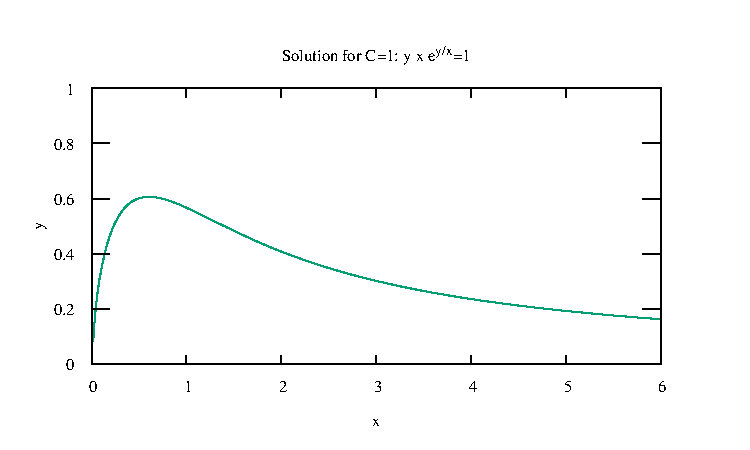
\includegraphics[width=0.5\textwidth] {../A/analysis/implicit_solution.pdf}
\item $\displaystyle y' = \frac{x^2y}{x^3+y^3}$.

With the substitution $u=y/x$ we have:
\begin{align*}
y'&=\frac{x^2y}{x^3+y^3},\\
y'&=\frac{y/x}{1+y^3/x^3},\\
y'&=\frac{u}{1+u^3},\\
y'&=u'x+u = \frac{u}{1+u^3},\\
u'&= \frac{1}{x}\left( \frac{u}{1+u^3} - u\right),\\
u'&= -\frac{1}{x}\left( \frac{u^4}{1+u^3}\right).
\end{align*}
The last equation can be solved by separation of variables and it leads to an implicit equation for $y$ after back substitution.
\item $\displaystyle y'=\frac{1}{x+y}$.

With the substitution $u=x+y$ we get
\begin{align*}
y'&=\frac{1}{u}\\
y'&=u'-1 =\frac{1}{u}\\
u' &= \frac{1+u}{u}.
\end{align*}
The last equation can be solved by separation of variables and it leads to an implicit equation for $y$ after back substitution.
\item $\displaystyle y'=-\sin^2(x+y+1)$.

With the substitution $u=x+y+1$ we get
\begin{align*}
y'&=-\sin^2(u)\\
y'&=u'-1 =-\sin^2(u)\\
u' &= \cos^2(u).
\end{align*}
This equation can be solved by separation of variables (solution not required by the exercise):
\begin{align*}
u' &= \cos^2(u),\\
\frac{\d u}{\cos^2(u)} &= \d x,\\
\int \frac{\d u}{\cos^2(u)} &= \int \d x,\\
\tan(u) &= x+C,\\
u &= \arctan(x+C),\\
y+x+1 &= \arctan(x+C),\\
y &= \arctan(x+C)-x-1.
\end{align*}

\item $\displaystyle x^2y' = y^2+xy-x^2$.

With the substitution $u=y/x$ we get 
\begin{align*}
y'&=\frac{y^2}{x^2}+\frac{y}{x} -1,\\
y'&=u'x+u = u^2+u-1,\\
u'&= \frac{u^2-1}{x}.
\end{align*}
This equation can be solved by separation of variables and partial fraction decomposition for example.

\item $\displaystyle y'=\frac{y+\operatorname{e}^{-\frac{y}{x}}}{x}$.

With the substitution $u=y/x$ we get

\begin{align*}
y'&=\frac{y}{x} + \frac{1}{x}\operatorname{e}^{-\frac{y}{x}},\\
y'&= u+\frac{1}{x}\operatorname{e}^{-u},\\
y'&= u'x+u = u+\frac{1}{x}\operatorname{e}^{-u},\\
u'&= \frac{1}{x^2}\operatorname{e}^{-u}.
\end{align*}
This can be solved by separation of variables.

\end{iii}

\end{itemize}
}




\ifthenelse{\boolean{mitLoes}}{\ruleBig \cleardoublepage}{}
%17
\Aufgabe[e]{Differentialgleichungen erster Ordnung}
{
\begin{itemize}
\item[\textbf{1)}] Klassifizieren Sie die follgenden gew\"ohnlichen Differentialgleichungen 
                   erster Ordnung als 

\begin{enumerate}
\item[\textbf{a)}] Linear oder nicht-linear.
\item[\textbf{b)}] In dem Fall einer linearen Differentialgleichung klassifizieren Sie 
                   die Gleichung zus\"atzlich als
\begin{itemize}
\item homogen oder inhomogen.
\item Differentialgleichung mit konstanten oder nicht-konstanten Koeffizienten.
\end{itemize}
\item[\textbf{c)}]  Nutzen Sie die Vorlesungsunterlagen, um die Differentialgleichung als
                    einen der folgenden Typen zu klassifizieren:
\begin{enumerate}
\item $y'= f(x)\cdot g(y)$, zu lösen mittels Trennung der Variablen,
\item $y'=g(y/x)$, homogen, zu l\"osen mittels Substitution mit $u=y/x$,
\item $y'=f(ax+by+c)$, rechte Seite mit bilinearen Argumenten, zu lösen mit der 
      Substitution $u=ax+by+c$,
\item $y'+p(x) \cdot y = q(x)$, lineare Differentialgleichung.
\end{enumerate}
\end{enumerate}
\begin{multicols}{2}
\begin{iii}
\item $y' + 2 y = 3x$.
\item $y'y + x = 0$.
\item $y'= \frac{x^2+y^2}{xy}$.
\item $y'=(x+y+1)^2$.
\item $x^2y'= x y + 2y^2$.
\item $y'=\frac{y(x-y)}{x^2}$.
\item $y'=\frac{x-y}{x+y}$.
\item $y'= \ln(y+2x+1)^2$.
\end{iii}
\end{multicols}
\item[\textbf{2)}] Berechnen Sie die allgemeine L\"osung der Gleichungen \textbf{i)} 
                   bis \textbf{iv)}.
\end{itemize}
}


\Loesung{
\begin{itemize}
\item[\textbf{1)}] 
\begin{iii}
\item $y' + 2 y = 3x$. Linear, inhomogen, mit konstanten Koeffizients, Typ: rechte 
      Seite mit bilinearen Koeffizienten.
\item $y'y + x = 0$. Nicht-linear, Typ: Trennung der Variablen.
\item $y'= \frac{x^2+y^2}{xy}$. Nicht-linear, Typ: homogen mit Substitution $u=y/x$.
%\item $x^2y' = 2y + 1$. Linear, inhomogeneous, non-constant coefficients, type D.
\item $y'=(x+y+1)^2$. Nicht-linear, Typ: rechte Seite mit bilinearen Argumenten.
\item $x^2y'= x y + 2y^2$. Nicht-linear, Typ: homogen mit Substitution $u=y/x$.
%\item $y' = \cos(x)y$. Linear, homogeneous, non-constant coefficients, type D.
\item $y'=\frac{y(x-y)}{x^2}$. Nicht-linear, Typ: homogen mit Substitution $u=y/x$.
\item $y'=\frac{x-y}{x+y}$. Nicht-linear, Typ: homogen mit Substitution $u=y/x$.
\item $y'= \ln(y+2x+1)^2$. Nicht-linear, Typ: rechte Seite mit bilineren Argumenten.
\end{iii}
\item[\textbf{2)}] Berechnen Sie die allgemeine L\"osung der Gleichungen \textbf{i)} und \textbf{ii)}.

\noindent Zu \textbf{i)}

\underline{Die Gleichung kann als lineare Gleichung gel\"ost werden:}
Die Gleichung ist linear, erster Ordnung, mit konstanten Koeffizienten und inhomogen.
% it is linear, first order, with constant coefficients and inhomogeneous.
Die L\"osung kann als Summe aus der L\"osung der homogenen Gleichung und einer partikul\"aren 
L\"osung bestimmt werden:
% The solution can be determined as the sum of the solution of the homogeneous equation and a particular solution: 
$$
y(x) = y_h(x) + y_p(x).
$$
Die Lösung der homogenen Gleichung mit dem allgemeinen Lösungsverfahren für den Fall mit 
nicht-konstanten Koeffizienten, den wir hier zeigen. Man kann die Lösung auch durch Berechnung 
der Nullstellen des charakteristischen Polynoms bestimmen. Dieser Methode wird später gezeigt.

% The solution of the homogeneous equation can be determined following the general solution procedure for the case with non-constant coeffcients as we do here to show the method. It could be also determined computing the zeros of the characteristic polynomial and this will be shown later.

\underline{Die Gleichung kann interpretiert werden vom Typ rechte Seite mit bilinearen}\\
\underline{Argumenten.}
% The equation can be also interpreted as type: right hand side with bilinear argument.}
$$
y'=f(ax+by+c)=3x-2y
$$
und wird mit der Substitution, wie unten gezeigt, gelöst.
% and solved with a substitution as shown below.

Wir beginnen mit der allgemeinen Methode. Die Lösung des homogenen Problems ist
% Let's start with the general method. The solution of the homogeneous problem is
$$
y_h(x) = C \operatorname{e}^{-P(x)},
$$
wobei
$$
P(x) = \int^x p(t) \d t
$$
und $p(x)$ in diesem Fall 2 ist, sodass $P(x) = 2x$ gilt und
$$
y_h(x) = C\operatorname{e}^{-2x}.
$$
Für die partikuläre Lösung nutzen wir die Methode der Variation der Konstanten
% For the particular solution with use the method of variations of constants
$$
y_p(x) = C(x) \operatorname{e}^{P(x)} = C(x) \operatorname{e}^{-2x}.
$$
Wir nutzen dieselbe Ansatzfunktion wie im homogenen Teil aber multipliziert mit der 
Funktion $C(x)$ statt der Konstanten $C$.
% We use the same ansatz function as in the homogeneous part but multiplied by the function $C(x)$ instead of the constant $C$.
Um den Ausdruck für $C(x)$ zu bestimmen, leiten wir $y_p(x)$ ab
% To determine the expression for $C(x)$ we derive $y_p(x)$
$$
y_p'(x) = C'(x) \operatorname{e}^{-2x} -2 C(x) \operatorname{e}^{-2x}
$$
und setzen $y$ und $y'$ in die Differentialgleichung ein
\begin{align*}
C'(x) \operatorname{e}^{-2x} -2 C(x) \operatorname{e}^{-2x} + 2 C(x) \operatorname{e}^{-2x} &= 3x\\
C'(x) \operatorname{e}^{-2x} &= 3x\\
C'(x) = 3x \operatorname{e}^{2x}\\
\int \d C = 3 \int x \operatorname{e}^{2x} \d x.
\end{align*}
Das Integral auf der rechten Seite  wird mit partieller Integration berechnet
% The integral on the right hand side is computed by integration by parts with
\begin{align*}
u=x, \quad u'&=1,\\
v'=\operatorname{e}^{2x}, \quad v&=\frac{1}{2}\operatorname{e}^{2x}.
\end{align*}
Es gilt
\begin{align*}
\int x \operatorname{e}^{2x} \d x &= \frac{1}{2} \operatorname{e}^{2x} - \int \frac{1}{2} \operatorname{e}^{2x} \d x\\
&= \frac{1}{2} \operatorname{e}^{2x} - \frac{1}{4} \operatorname{e}^{2x} + \tilde C\\
&= \frac{1}{2}\operatorname{e}^{2x} ( x - \frac{1}{2}) + \tilde C.
\end{align*}
Zurück zu dem Integral
% Coming back to the integral
$$
\int \d C = 3 \int x \operatorname{e}^{2x} \d x,
$$
erhalten wir
$$
C(x) = \frac{3}{2} \operatorname{e}^{2x} (x-\frac{1}{2}) + \tilde C.
$$
Die Konstante $\tilde C$ kann null gesetzt werden, weil sie bereits in der Lösung der 
homogenen Gleichung berücksichtigt wurde.
% The constant $\tilde C$ can be set to zero, because it is already present in the solution of the homogeneous equation. 

Die partikuläre Lösung ist
% The particular solution is
\begin{align*}
y_p(x) &= C(x) \operatorname{e}^{-2x} = \left( \frac{3}{2} \operatorname{e}^{2x} (x-\frac{1}{2})\right) \operatorname{e}^{-2x}\\
&=\frac{3}{2} (x-\frac{1}{2}).
\end{align*}
Die allgemeine Lösung ist
% The general solution is
$$
y(x) = y_h(x) + y_p(x) = C \operatorname{e}^{-2x} + \frac{3}{2} (x-\frac{1}{2}).
$$

\underline{Wir lösen die Gleichung nun als Typ: rechte Seite mit bilinearen}\\
\underline{Argumenten.}
$$
y'=f(ax+by+c)=3x-2y.
$$
Mit der Substitution $u=3x-2y$, erhalten wir
$$
u'= 3 -2y'.
$$
Da $y'=3x-2y=u$ gilt 
$$
u'= 3-2u.
$$
Diese lösen wir mit Trennung der Variablen
% This can be solved by separation of variables
\begin{align*}
\frac{\d u}{\d x} &= 3-2u\\
 \int \frac{\d u}{3-2u} &= \int \d x\\
 -\frac{1}{2} \ln |3-2u| &= x + C\\
 -\frac{1}{3-2u} &= C\operatorname{e}^{2x},
\end{align*}
mit der Rücksubstitution erhalten wir
% by back substitution it is
\begin{align*}
\frac{1}{3-6x+4y} &= C \operatorname{e}^{2x}\\
3-6x+4y &= C \operatorname{e}^{-2x}\\
y &= C\operatorname{e}^{-2x} +\frac{3}{2}x - \frac{3}{4}.
\end{align*}

\newpage
\underline{Die Differentialgleichung gelöst werden als lineare Differentialgleichung mit}\\
\underline{ konstanten Koeffizienten:}

Wir bestimmen das charakteristische Polynom
% We derive the characteristic polynomial
$$
p(\lambda) = \lambda + 2
$$
mit den Nullstellen $\lambda = -2$. Damit ist die Lösung der homogenen Gleichung 
$$
y_h(x) = C\operatorname{e}^{\lambda x} = C \operatorname{e}^{-2x}.
$$
Der Ansatz für die partikuläre Lösung ist
$$
y_p(x) = A_1x + A_0.
$$
Durch Ableiten erhalten wir
$$
y_p'(x) = A_1.
$$
Wir setzen $y_p$ und $y_p'$ in die Differentialgleichung ein und erhalten
% Inserting $y_p$ and $y_p'$ into the ODE we get
$$
A_1+2A_1x+2A_0 = 3x.
$$
Ein Koeffizientenvergleich liefert
% and equating the coeffcients we get
\begin{align*}
2A_1 &= 3\\
A_1+2A_0 &= 0
\end{align*}
wodurch wir die Werte $A_0 = -\frac{3}{4}$ und $A_1 = \frac{3}{2}$ erhalten und 
die partikuläre Lösung
$$
y_p(x) = \frac{3}{2}x-\frac{3}{4}.
$$
Die allgemeine Lösung ist wieder
$$
y(x) = y_h(x)+y_p(x) = C\operatorname{e}^{-2x} + \frac{3}{2}x-\frac{3}{4}.
$$
\noindent Zu \textbf{ii)}

Die Gleichung
$$
y'y = -x,
$$
ist vom \underline{Typ: Trennung der Variablen}
\begin{align*}
\int y \d y &= -\int x \d x\\
\frac{y^2}{2} &= -\frac{x^2}{2}+\widetilde C\\
y^2 &= C-x^2, \quad C = 2\widetilde C,\\
y &= \pm \sqrt{C-x^2}.
\end{align*}
Die Gleichung $y'y-x=0$ kann auch interpretiert werden als\\
\underline{Typ: nicht-linear, homogen mit der Substitution $u=y/x$}
$$
y' = -\frac{x}{y}
$$ 
und kann mit der Substitution $u=\frac{y}{x}$ gelöst werden.

Aus der Beziehung $ux = y$, erhalten wir durch differenzieren beider Seiten
$$
u' x + u = y',
$$
wobei wir die Produktregel benutzen.
% where we have used the product rule for the product $ux$.
Mit der Substitution $y'=-\frac{1}{u}$ erhalten wir
\begin{align*}
u'x + u &= - \frac{1}{u}\\
u' &= -\frac{1}{x} (u+\frac{1}{u})\\
\int \frac{u}{u^2+1}\d u &= \int -\frac{1}{x}\d x\\
\frac{1}{2}\ln (u^2+1) &= -\ln x + \ln \widetilde C\\
u^2+1 &= \frac{C}{x^2}, \quad C=\widetilde C^2\\
u^2 &= \frac{C}{x^2}-1,
\end{align*}
durch die Rücksubstitution erhalten wir
\begin{align*}
u^2 &= \frac{C}{x^2}-1,\\
\frac{y^2}{x^2} &= \frac{C}{x^2}-1,\\
y^2 & = C -x^2\\
y&=\pm \sqrt{C-x^2}.
\end{align*}

\end{itemize}
}




\ifthenelse{\boolean{mitLoes}}{\ruleBig \cleardoublepage}{}
\newpage
%18
\Aufgabe[e]{Differentialgleichungen erster Ordnung}
{
Klassifizieren Sie die folgenden Differentialgleichungen erster Ordnung:
\begin{multicols}{2}
\begin{enumerate}
\item $x^2y' = 2y + 1$. 
\item $y' = \cos(x)y$. 
\item $x^2 y' + y^2 = x y$.
\item $y'=\sin(y+1)$. 
\item $y'=(4x-y+1)^2$.
\item $y'+3y+2=\operatorname{e}^{2x}$. 
\end{enumerate}
\end{multicols}
%
\begin{abc}
\item Klassifizieren Sie diese als linear oder nicht linear.
In dem Fall einer linearen Differentialgleichung klassifizieren Sie die zusätzlich als
\begin{iii}
\item homogen oder inhomogen.
\item mit konstanten oder nicht-konstanten Koeffizienten.
\end{iii}
\item Klassifizieren Sie die Differentialgleichung als einen der folgenden Typen:
\begin{iii}
\item $y'= f(x)\cdot g(y)$ zu Lösen mit Trennung der Variablen.
\item $y'=g(y/x)$ zu Lösen mit der Substitution $u=y/x$.
\item $y'=f(ax+by+c)$ zu Lösen mit der Substitution $u=ax+by+c$.
\item $y'+p(x) \cdot y = q(x)$.
\end{iii}
\item Berechnen Sie die allgemeine Lösung aller Differentialgleichungen.
\end{abc}
}


\Loesung{
\begin{itemize}
\item[\textbf{1)}] 
\begin{iii}
\item $x^2y' = 2y + 1$. Linear, inhomogen, nicht-konstant Koeffizienten: Typ A (separabel) 
oder Typ D.
\item $y' = \cos(x)y$. Linear, homogen, nicht-konstant Koeffizienten, separabel (Typ A).
\item $x^2 y' + y^2 = x y(x)$. Nicht-linear, homogen, lösbar mit der Substitution von  Typ B.
\item $y'=\sin(y+1)$. Nicht-linear, separabel von Typ A.
\item $y'=(4x-y+1)^2$. Nicht-linear, Typ C.
\item $y'+3y+2=\operatorname{e}^{2x}$. Linear, inhomogen, Typ D mit konstanten Koeffizienten.
\end{iii}
\item[\textbf{2)}] 
\begin{iii}
\item $x^2y' = 2y + 1$. Linear, inhomogen, nicht-konstant Koeffizienten: Typ A (separabel)

\begin{align*}
\frac{\d y}{2y+1} &= \frac{\d x}{x^2},\\
\frac{1}{2} \ln(2y+1) &= -\frac{1}{x},\\
2y+1 &= \widetilde C\operatorname{e}^{-\frac{2}{x}},\\
y &= C e^{-\frac{2}{x}} -\frac{1}{2}.
\end{align*}

Diese Gleichung kann auch mit einem längeren Verfahren gelöst werden, wenn man sie als vom Typ D betrachtet: Zuerst wird die Lösung des homogenen Teils (H) bestimmt und dann die besondere Lösung (P) mit der Methode der unbestimmten Koeffizienten.
Wir beginnen mit (H):
Die Gleichung  
$$x^2y'=2y$$
ist separabel und sie hat die Lösung
$$
y_h(x) = C e^{\frac{-2}{x}}.
$$
Für den Teil (P) machen wir den Ansatz
$$
y_p(x) = C(x) e^{\frac{-2}{x}}.
$$
Dann leiten wir ab:
$$
y_p'(x) = C'(x) e^{\frac{-2}{x}} + C(x) \frac{2}{x^2} e^{\frac{-2}{x}}.
$$
Einsetzen in die Gleichung ergibt
\begin{align*}
C'(x) x^2 e^{\frac{-2}{x}} + 2C(x) e^{\frac{-2}{x}} &= 2 C(x) e^{\frac{-2}{x}} +1\\
C'(x) x^2 e^{\frac{-2}{x}} &= 1\\
C'(x) &= \frac{e^{\frac{2}{x}}}{x^2}\\
\int \d C &= \int \frac{e^{\frac{2}{x}}}{x^2}\d x.
\end{align*}
Wir integrieren das Integral auf der rechten Seite mit der Substitution $u=2/x$, woraus wir das Differential $\d u = -\frac{2}{x^2}\d x$ berechnen. Wir haben also
$$
\frac{\d x}{x^2} = -\frac{\d u}{2} 
$$
und
\begin{align*}
\int \d C &=  -\frac{1}{2} \int e^u \d u,\\
C &=  -\frac{1}{2} e^u + \widetilde C,\quad \text{ (z.B. } \widetilde C = 0)\\
C &=  -\frac{1}{2} e^\frac{2}{x}.\quad \text{ (nach Rücksubstitution)}
\end{align*}
Daher ist die partikuläre Gleichung
$$
y_p(x) = -\frac{1}{2}  e^\frac{2}{x}  e^\frac{-2}{x} =  -\frac{1}{2}
$$
und die allgemeine Lösung ist
$$
y(x) = y_h(x) + y_p(x) = C e^\frac{-2}{x} - \frac{1}{2}.
$$
\item $y' = \cos(x)y$. Linear, homogen, nicht-konstant Koeffizienten, separabel (Typ A).

Lösung:
\begin{align*}
\int \frac{1}{y} \d y &= \int \cos(x) \d x,\\
\ln(y) &= \sin(x) + \ln(C),\\
y &= C e^{\sin(x)}.
\end{align*}
\item $x^2 y' + y^2 = x y(x)$. Nicht-linear, homogen, lösbar mit der Substitution von  Typ B.

Die Gleichung kann umgeformt werden zu
$$
y'= \frac{y}{x} -\frac{y^2}{x^2}.
$$
Mit der Substitution $u=y/x$ erhalten wir 
\begin{align*}
y&=u x\\
y'&=u' x + u.
\end{align*}
Wir substituieren $y'$ und $y/x$ in die Differentialgleichung und erhalten
$$
u' x + u = u -u^2.
$$
Diese kann mit Seperation der Variablen gelöst werden.
%
\begin{align*}
u' &= -\frac{u^2}{x},\\
\int \frac{1}{u^2} \d u &= -\frac{1}{x} \d x,\\
-\frac{1}{u} &= \ln(x) + C,\\
u &= \frac{1}{\ln(x) + C},\\
y &= \frac{x}{\ln(x) + C}. \quad (\text{ nach Rücksubstitution } u=y/x)
\end{align*}
%
\item $y'=\sin(y+1)$. Nicht-linear, separabel von Typ A.

Wir lösen die Differentialgleichung mit Trennung der Variablen:
%
\begin{align*}
\int \frac{\d y}{\sin(y+1)} &= \int \d x,\\
\ln|\tan\left(\frac{y+1}{2}\right)| &= x + \ln(C),\\
\tan\left(\frac{y+1}{2}\right) &= C e^x,\\
\frac{y+1}{2} &= \arctan(Ce^x),\\
y &= 2\arctan(Ce^x)-1.
\end{align*}
%
\item $y'=(4x-y+1)^2$. Nicht-linear, Typ C.

Diese nichtlinesre Differentialgleichung kann mit Substitution gelöst werden. Wir setzen
$$
u = 4x-y+1
$$
und erhalten
$$
u'= 4-y' \quad \rightarrow \quad y'=4-u'.
$$
Substituieren $u=4x-y+1$ und $y'=4-u'$ in die Gleichung, führt zu der seperablen 
Gleichung
\begin{align*}
4-u' &= u^2,\\
u' & = 4-u^2,\\
\frac{\d u}{4-u^2} &= \d x,\\
\int \frac{\d u}{4-u^2} &= \int \d x,\\
\frac{1}{4} \ln|u+2| - \ln|u-2| &= x+ \ln(\widetilde C), \quad \text{ (mit Partialbruchzerlegung, siehe unten)}\\
\ln\frac{u+2}{u-2} &= 4x + \ln(\widetilde C^4),\\
u+2 &= Ce^{4x}(u-2),\quad (\text{mit } C=\widetilde C^4)\\
u & = -2Ce^{4x} + uCe^{4x} -2,\\
u(1-Ce^{4x}) &= -2\left(Ce^{4x}+1\right)\\
u &= -2 \frac{Ce^{4x}+1}{1-Ce^{4x}},\\
4x-y+1 &= -2 \frac{Ce^{4x}+1}{1-Ce^{4x}}, \quad \text{(Rücksubstitution)}\\
y &= 4x + \frac{3+Ce^{4x}}{1-Ce^{4x}}.
\end{align*}
%
Für die Partialbruchzerlegung im 5. Schritt oben ergibt sich
$$
\frac{-1}{u^2-4} = -\frac{1}{4} \frac{1}{x-2} + \frac{1}{4} \frac{1}{x+2}.
$$
%
\item $y'+3y+2=\operatorname{e}^{2x}$. Linear, inhomogen, Typ D mit konstanten Koeffizienten.

Diese Gleichung kann als Typ D mit der Methode der unbestimmten Koeffizienten oder als lineare inhomogene ODE mit konstanten Koeffizienten gelöst werden, wobei spezielle Ansätze für die Inhomogenitäten und das Superpositionsprinzip verwendet werden.

Beginnen wir mit der ersten Methode. Hier müssen wir das homogene Problem (H) lösen und dann eine partikuläre Lösung (P) finden.

Für das homogene Problem können wir die Variablentrennung verwenden oder im Falle konstanter Koeffizienten (nur in diesem Fall!) das charakteristische Polynom benutzen:
$$
\lambda + 3 = 0 \quad \rightarrow \quad \lambda = -3
$$
um den Lösungsteil zu bestimmen
$$
y_h(x) = C e^{-3x}.
$$
Um das Problem (P) zu lösen, machen wir den Ansatz
$$
y_p(x) = C(x) e^{-3x}
$$
und differentieren ihn
$$
y_p'(x) = C'(x) e^{-3x} - C(x) 3 e^{-3x}.
$$
Wir setzen $y_p$ und $y_p'$ in die gleichung ein und erhalten
\begin{align*}
C'(x)e^{-3x} -3C(x) e^{-3x} +3Ce^{-3x} +2 &= e^{2x}\\
C'(x)&= e^{5x}-2e^{3x}\\
C(x) &= \frac{1}{5}e^{5x} -\frac{2}{3}e^{3x}.
\end{align*}
Die partikuläre Lösung ist
$$
y_p(x) = \left( \frac{1}{5}e^{5x} -\frac{2}{3}e^{3x} \right) e^{-3x} = \frac{1}{5}e^{2x}  -\frac{2}{3}
$$
un die allgemeine Lösung ist
$$
y(x) = y_h(x) + y_p(x) = C e^{-3x} +  \frac{1}{5}e^{2x}  -\frac{2}{3}.
$$

Wie bereits erwähnt, können wir das Problem mit Hilfe spezieller Ansätze für die Inhomogenitäten und dem Superpositionsprinzip lösen.

Die rechte Seite der Gleichung ist $e^{2x} -2$, also finden wir zwei Lösungen für die beiden Terme getrennt. Zunächst für $e^{2x}$. Der Ansatz im exponentiellen Fall ist wieder exponentiell $y_{p1}=Ae^{\alpha x}$, wobei $\alpha$ der Exponent des rechten Terms ist:
$$
y_{p1} = A e^{2x}.
$$
Die Konstante $A$ wird durch Koeffizientenvergleich gefunden:
\begin{align*}
y_{p1}' +3y_{p1} &= e^{2x}, \quad \text{(Bemerkung: der Term -2 wird nicht betrachtet)}\\
2 A e^{2x} + 3 A e^{2x} &= e^{2x},\\
A &= \frac{1}{5}.
\end{align*}
Der erste Teil der partikulären Lösung ist

$$
y_{p1} = \frac{1}{5}e^{2x}.
$$
Der zweite Teil wird mit dem Polynom-Ansatz nullter Ordnung $y_{p2}=B$ berechnet, da der Term $-2$ eine Konstante ist. Setzt man die Ansatzfunktion in die Differentialgleichung ein, so erhält man
$$
3 B = -2 \quad B=-\frac{2}{3}.
$$
Wir haben also die partikuläre Lösung durch Superposition
$$
y_p(x) = y_{p1}(x) + y_{p2}(x) =  \frac{1}{5}e^{2x} - \frac{2}{3}
$$
un die allgemeine Lösung
$$
y(x) = y_h(x) + y_p(x) = Ce^{-3x} +  \frac{1}{5}e^{2x} - \frac{2}{3}.
$$
\end{iii}

\end{itemize}
}




\ifthenelse{\boolean{mitLoes}}{\ruleBig \cleardoublepage}{}
%19
\Aufgabe[e]{Trennung der Veränderlichen und Anfangswertproblem}

{
Klassifizeren die folgende Differentialgleichung und bestimmen Sie die Lösung des Anfangswertproblems mit $y(0) = 0$ und $y'(0) = 6$:
 $$
 y''(x) - 2 y'(x) - 3y(x) = 0.
 $$
}

\Loesung{
Die Nullstellen des charakteristischen Polynoms
$p(\lambda)=\lambda^2-2\lambda-3$ sind $\lambda_1=-1$ und $\lambda_2=3$.

Die allgemeine Lösung ist
$$ y(x) = c_1 \operatorname{e}^{-x} + c_2 \operatorname{e}^{3x}  \text{ mit } c_1,c_2 \in \mathbb{R} .$$

Mit den Anfangswertbedingungen $y(0)=c_1 + c_2 \stackrel{!}{=} 0$ und 
$y^\prime(0) = -c_1 + 3c_2 \stackrel{!}{=} 6$ erhalten wir das lineare System
% $$ \begin{array}{rcrl}
$$ \begin{array}{rcrl}
   c_1 & + & c_2 & = 0, \\
  -c_1 & + & 3c_2 & = 6 
   \end{array} $$
mit Lösung $c_2=3/2$ und $c_1=-3/2$. Damit ist 
$$ y(x) = -\frac32  \operatorname{e}^{-x} + \frac32 \operatorname{e}^{3x}. $$
%    \end{array} $$
% with solution $c_2=3/2$ and $c_1=-3/2$. This yields
% $$ y(x) = -\frac32  \operatorname{e}^{-x} + \frac32 \operatorname{e}^{3x}. $$

}


\ifthenelse{\boolean{mitLoes}}{\ruleBig \cleardoublepage}{}
%20
\Aufgabe[e]{Homogene lineare Differentialgleichungen}
{
Bestimmen Sie die allgemeinen reellen Lösungen folgender homogener linearer Differentialgleichungen mit konstanten Koeffizienten mit Hilfe
geeigneter Ansätze für \ $u(t)$\,: 
\begin{align*}
\mathbf{i)} &  & u''-7\,u'+10\,u=0\;. & \;\; & 
\mathbf{ii)} &  & 7\,u''+28\,u'+91\,u=0\;. \\ 
\mathbf{iii)} &  & u'''-3\,u''=0\;. &  & 
\mathbf{iv)} &  & u''''+8\,u''+16\,u=0\;.
\end{align*}
}

\Loesung{
Der Ansatz ist jedesmal \ \ $u(t)=\alpha \,\EH{\lambda \,t}\ ,\ \ \alpha,\lambda =\ $const$\,\in \mathbb{C}\ .$


\begin{enumerate}
\item[\textbf{i)}]  Die charkt. Gl. ist: \ \ \ $\lambda ^{2}-7\lambda+10=0 \Rightarrow \lambda _{1}=2\;,\;\;\lambda _{2}=5\ .$
\[
\Rightarrow \underline{\;u(t)=a\,\text{e}^{2\,t}+b\,\EH{5\,t}\;,\;\;a,b\in \mathbb{R}\;}\;. 
\]

\item[\textbf{ii)}]  Die charkt. Gl. ist: \ \ \ $\lambda ^{2}+4\lambda+13=0 \Rightarrow \lambda _{1,2}=-2\pm 3\,$i$\;.$%
\[
\Rightarrow \underline{\;u(t)=\text{e}^{-2\,t}\,\big(a\,\cos(3t)+b\,\sin (3t)\big)\;,\;\;a,b\in \Bbb{R}\;}\;. 
\]

\item[\textbf{iii)}]  Die charkt. Gl. ist: \ \ \ $\lambda ^{3}-3\lambda^{2}=0 \Rightarrow \lambda _{1,2}=0\;,\;\;\lambda _{3}=3\;.$
\[
\Rightarrow \underline{\;u(t)=a+b\,t+c\,\EH{3\,t}\;,\;\;a,b,c\in \Bbb{R}\;}\;. 
\]

\item[\textbf{iv)}]  Die charkt. Gl. ist:\ \ \ \ $\lambda ^{4}+8\lambda^{2}+16=0 \Rightarrow \lambda_{1,2}=2\,$i$\;,\;\;\lambda_{3,4}=-2\,$i$\;.$ 
\[
\Rightarrow \underline{\;u(t)=(a+b\,t)\cdot \cos (2t)+(c+d\,t)\cdot\sin (2t)\;,\;\;a,b,c,d\in \Bbb{R}\;}\;. 
\]
\end{enumerate}
}

\ErgebnisC{gewdglHomgLine001}{
\begin{iii}
\item $u(t)=a\,\text{e}^{2\,t}+b\,\EH{5\,t}$ 
\item $u(t)=\text{e}^{-2\,t}\,\big(a\,\cos(3t)+b\,\sin (3t)\big)$
\item $u(t)=a+b\,t+c\,\EH{3\,t} $
\item $u(t)=(a+b\,t)\cdot \cos (2t)+(c+d\,t)\cdot\sin (2t)$
\end{iii}
}

\ifthenelse{\boolean{mitLoes}}{\ruleBig \cleardoublepage}{}
%21
\Aufgabe[e]{Komplexe Nullstellen des charakteristischen Problems}
{
Bestimmen Sie die Lösung der folgenden Differentialgleichung:
% Determine the solution of the following differential equation:
$$y^{\prime\prime}+4y^\prime+5y=0$$
}

\Loesung{
\begin{abc}
\item 
Das charakteristische Polynom $p(\lambda)=\lambda^2+4\lambda+5$ hat die Nullstellen
$$\lambda_1=-2+i, \lambda_2=-2-i$$
die Lösung ist dann
\begin{align*}
y&=C_1\EH{-2t+\imag t}+C_2\EH{-2t-\imag t}\\
&= \EH{-2t}(C_1(\cos t+\imag \sin t)+C_2(\cos t-\imag \sin t)) \\
&= \EH{-2t}(c_1\cos t+c_2 \sin t )
\end{align*}
wobei die reellem Konstanten $c_1=C_1+C_2$ und $c_2 = i(C_1-C_2)$ sind.

Die komplexen Konstanten können durch die rellen Konstanten wie folgt ausgedrückt werden:
$C_1=\overline{C_2}=\dfrac{c_1-\imag c_2}{2}$.
\end{abc} 
}


\ErgebnisC{AufggewdglLinenOrd002}
{
a) $y(x) = c_1 \EH{2x}+c_2\EH{-x}$
}


\ifthenelse{\boolean{mitLoes}}{\ruleBig \cleardoublepage}{}
%22
\Aufgabe[e]{Lineare Differentialgleichungen $n$-ter Ordnung}
{
Bestimmen Sie die allgemeinen L\"osungen der folgenden
Differentialgleichungen:
% \begin{abc}
% \item $y^{(4)} + 4y = 0$,
% \item $y^{(4)} + 2y''' + y'' = 12 x$,
% \item $y^{\prime\prime}+4y^\prime+5y=8\sin t$,
% \item $y^{\prime\prime}-4y^\prime+4y=\EH{2x}$.
% \Aufgabe[e]{Linear ODEs of the 4th order}
% {
% Compute the general solutions of the following
% differential equations:
\begin{abc}
\item $y^{(4)} + 4y = 0$,
\item $y^{(4)} - 18 y'' + 81y=0$.
\end{abc}
}

\Loesung{
\begin{abc}
% \item Es ist $p(\lambda)=\lambda^4+4$, die Nullstellen sind 
% $\lambda_\ell = \sqrt{2} \EH{i (2\ell+1) \pi / 4}$ für $\ell=0,1,2,3$,
% also $$\lambda_0=1+i, \lambda_1=-1+i, \lambda_2=-1-i, \lambda_3=1-i$$
% Ein reelles Fundamentalsystem ist
% $$\{ e^x \cos x, e^x \sin x, \EH{-x} \cos x, \EH{-x} \sin x \}$$ 
% Die allgemeine Lösung lautet also
% $$ y(x) = c_1 e^x \cos x + c_2 e^x \sin x + c_3 \EH{-x} \cos x 
%    + c_4 \EH{-x} \sin x \text{ mit } c_1,c_2,c_3,c_4 \in \R . $$
\item Das characteristische Polynom ist $p(\lambda)=\lambda^4+4$, mit den Nullstellen
%$\lambda_\ell = \sqrt{2} \EH{i (2\ell+1) \pi / 4}$ for $\ell=0,1,2,3$,
$\lambda_\ell = \sqrt{2} \EH{i (\pi/2+k\pi) / 2}$ for $k=0,1,2,3$,
$$\lambda_0=1+i, \lambda_1=-1+i, \lambda_2=-1-i, \lambda_3=1-i.$$
Das Fundamentalsystem ist dann
$$\{ e^x \cos x, e^x \sin x, \EH{-x} \cos x, \EH{-x} \sin x \}$$ 
Die allgemeine Lösung ist also gegeben als
% The general solution is therefore given as
$$ y(x) = c_1 e^x \cos x + c_2 e^x \sin x + c_3 \EH{-x} \cos x 
   + c_4 \EH{-x} \sin x \text{ with } c_1,c_2,c_3,c_4 \in \R . $$
\item
Von der gegebenen Gleichung $$y^{(4)} - 18 y'' + 81y=0,$$
ist das characteristische Polynom
$$
\lambda^4-18\lambda + 81 = 0
$$
und kann geschrieben werden als
$$
(x^2-9)^2 = (x-3)^2\cdot(x+3)^2 = 0
$$
mit den zwei doppelten Nullstellen: $\lambda_1 = -3$ und $\lambda_2 = 3$.
Die allgemeine Lösung der hommogenen Differentialgleichung ist
% The general solution of the homogeneous ODE is
$$
y(x) = (c_1+c_2x) e^{-3 x} + (c_3 + c_4x) e^{3 x}.
$$
Die Koeffizienten vor der Exponentialfunktion sind lineare Funktionen, weil es sich um doppelte Nulstellen handelt.
% % Here we observe that the coefficients in front of the exponential functions are linear functions because the multiplicity of the zeros is 2.
\end{abc} 
}


\ErgebnisC{AufggewdglLinenOrd003}
{
Partikuläre Lösungen:
a) $0$, \, 
b) $-12x^2+2x^3$,\, 
c) $\sin t-\cos t$,\, 
d) $\frac 12 x^2\EH{2x}$
% {
% Particulate solutions:
% a) $0$, \,
% b) $-12x^2+2x^3$,\,
% c) $\sin t-\cos t$,\,
% (d) $\frac 12 x^2\EH{2x}$
}


\ifthenelse{\boolean{mitLoes}}{\ruleBig \cleardoublepage}{}
%23
\Aufgabe[e]{homogene lineare Dgl. h\"oherer Ordnung}
{
L\"osen Sie die homogenen Differentialgleichungen mit Hilfe des Exponentialansatzes
$$
y(t) = c e^{\lambda t}, \, c, \lambda = \text{const.}. 
$$

\begin{abc}
\item $y''-3y'+2y=0$
\item $y''+4y=0$
\item $y''+2y'+2y=0$
\item $y^{(4)}-y=0$
\end{abc}
}

\Loesung{
\begin{abc}
\item Einsetzen des Exponentialansatzes in die hom. lin. Dgl. mit konstanten Koeffizienten ergibt das charakteristische Polynom
$$
p(\lambda) = \lambda^2-3\lambda+2,
$$
das die Nullstellen $\lambda_1=1$ und $\lambda_2=2$ besitzt. Die allgemeine L\"osung ist die Linearkombination der beiden Fundamentall\"osungen $y_1(x)=e^x$ und $y_2(x)=e^{2x}$
$$
y(x)=c_1e^{x}+ c_2 e^{2x} \, \text{mit} \, c_1, c_2 \in \mathbb{R}.
$$

\item Aus $p(\lambda) = \lambda^2+4=0$ erh\"alt man $\lambda_{1,2}= \pm 2i$ und damit die reelle L\"osung
$$
y(x) = c_1 \cos(2x) +c_2 \sin(2x) \, \text{mit} \, c_1, c_2 \in \mathbb{R}.
$$

\item Aus $p(\lambda) = \lambda^2+2\lambda+2=0$ erh\"alt man $\lambda_{1,2}= -1 \pm i$. Ein reelles Fundamentalsystem ist ${e^{-x}\cos(x), e^{-x}\sin(x)}$. Die allgemeine L\"osung ist eine gedm\"ampfte Schwingung
$$
y(x) = (c_1 \cos(2x) +c_2 \sin(2x))e^{-x} \, \text{mit} \, c_1, c_2 \in \mathbb{R}.
$$

\item Mit $p(\lambda) = \lambda^4-1=(\lambda^2-1)(\lambda^2+1)=(\lambda-1)(\lambda+1)(\lambda-i)(\lambda+i)$ erh\"alt man die allgemeine reelle L\"osung
$$
y(x) = c_1 e^x +c_2 e^{-x} + c_3 \cos(x) + c_4 \sin(x) \, \text{mit} \, c_1, c_2, c_3, c_4 \in \mathbb{R}.
$$

\end{abc}
}


\ErgebnisC{gewdgl_homDgl}{
\begin{abc}
\item $y(x)=c_1e^{x}+ c_2 e^{2x} \, \text{mit} \, c_1, c_2 \in \mathbb{R}$
\item $y(x) = c_1 \cos(2x) +c_2 \sin(2x) \, \text{mit} \, c_1, c_2 \in \mathbb{R}$
\item $y(x) = (c_1 \cos(2x) +c_2 \sin(2x))e^{-x} \, \text{mit} \, c_1, c_2 \in \mathbb{R}$
\item $y(x) = c_1 e^x +c_2 e^{-x} + c_3 \cos(x) + c_4 \sin(x) \, \text{mit} \, c_1, c_2, c_3, c_4 \in \mathbb{R}$
\end{abc}
}


\ifthenelse{\boolean{mitLoes}}{\ruleBig \cleardoublepage}{}
%24
\Aufgabe[e]{Harmonischer Oszillator}
{\label{aufgabe:oszillator}
Man betrachte die Differentialgleichung
\[
y'' + 2\rho y' + \omega^2 y = 0, \quad \text{mit } \rho, \omega \in \mathbb R_+
\]
Die gegebene Differentialgleichung, ist eine klassische Form einer linearen Differentialgleichung zweiter Ordnung mit konstanten Koeffizienten. Aus physikalischer Sicht beschreibt diese Gleichung typischerweise gedämpfte harmonische Bewegungen, wobei:
\begin{itemize}
  \item \( y(t) \) die Verschiebung des Systems vom Gleichgewicht über die Zeit darstellt.
  \item \( \rho \) (der Koeffizient der ersten Ableitung \( y' \)) repräsentiert den Dämpfungsfaktor, der beeinflusst, wie schnell das System Energie durch Reibung oder andere resistive Kräfte verliert.
  \item \( \omega^2 \) (der Koeffizient von \( y \)) steht im Zusammenhang mit der Steifigkeit des Systems oder der Kraft, die es ins Gleichgewicht zurückführt. Der Parameter \( \omega \) selbst wird oft als natürliche Frequenz des ungedämpften Systems betrachtet.
\end{itemize}

\textbf{Physikalische Interpretationen}
\begin{enumerate}
  \item \textbf{Mechanische Systeme:} In der Mechanik kann diese Gleichung ein Masse-Feder-Dämpfer-System modellieren, bei dem eine Masse an einer Feder und möglicherweise einem Dämpfungselement (wie einem Stoßdämpfer) befestigt ist. Die Masse oszilliert um eine Gleichgewichtsposition, wobei die Feder eine rückstellende Kraft proportional zur Verschiebung liefert und der Dämpfer eine Kraft proportional zur Geschwindigkeit bereitstellt, die der Bewegung entgegenwirkt.

\begin{center}
\begin{tikzpicture}
    % Draw the wall
    \fill[gray] (-1,0) rectangle (-0.5,2.5);
    \draw[thick] (-1,0) -- (-1,2.5);

    % Draw the spring
    \draw[thick,decorate,decoration={coil,aspect=0.3,segment length=3mm,amplitude=3mm}] (-1,2) -- (2,2) node[midway,above=4mm] {Feder};

    % Draw the damper
    \draw[thick] (-1,0.5) -- (0,0.5) -- (0,1.5);
    \draw[thick] (0,1.5) -- (2,1.5) node[midway,above=-6mm] {D\"ampfer};

    % Draw the mass
    \fill[blue!20!white] (2,0) rectangle (3.5,2.5);
    \draw[thick] (2,0) -- (2,2.5) -- (3.5,2.5) -- (3.5,0) -- cycle;
    \node at (2.75,1.25) {Masse};

    % Ground and vertical lines
    \draw[thick] (-1,0) -- (4,0);
    \draw[dashed] (-0.75,0) -- (-0.75,2);
    \draw[dashed] (2.75,0) -- (2.75,2);
    
    % Distance annotation
    \draw[<->] (-0.75,-0.5) -- (2.75,-0.5) node[midway,fill=white] {x};
\end{tikzpicture}
\end{center}


  \item \textbf{Elektrische Schaltkreise:} In der Elektrotechnik kann die Gleichung einen RLC-Schaltkreis (einen Schaltkreis, der einen Widerstand \( R \), eine Induktivität \( L \), und einen Kondensator \( C \) enthält) beschreiben. Hier könnte \( y(t) \) die elektrische Ladung oder den Strom darstellen, \( 2 \rho = R/L \) und \( \omega^2 = 1/(LC)\). Das Verhalten des Schaltkreises — ob er oszilliert oder schnell stabilisiert wird — hängt von den Werten dieser Komponenten ab.

\begin{center}
\begin{circuitikz}
    \draw
    % Voltage source
    (0,0) to[V, v=$V_s$, invert] (0,3)
    % Resistor
    to[R, l=$R$, v<=$V_R$] (3,3)
    % Inductor
    to[L, l=$L$, v<=$V_L$] (6,3)
    % Capacitor
    to[C, l=$C$, v<=$V_C$] (6,0)
    % Connect back to the voltage source
    -- (0,0);

    % Labels
    \node at (3,1.5) {RLC Stromkreis};
\end{circuitikz}
\end{center}
\end{enumerate}
Diese Gleichung ist allgemein bekannt als \textit{"Gedämpfter harmonischer Oszillator"} oder einfach als \textit{"Gedämpfter Oszillator"}. Sie umfasst drei spezifische Szenarien basierend auf dem Wert von \( \rho \) im Vergleich zu \( \omega \):
\begin{enumerate}
  \item \textbf{Überdämpft (\( \rho > \omega \)):} Das System kehrt ohne Oszillation langsam zum Gleichgewicht zurück.
  \item \textbf{Kritisch gedämpft (\( \rho = \omega \)):} Das System kehrt so schnell wie möglich ohne Oszillation zum Gleichgewicht zurück.
  \item \textbf{Untergedämpft (\( \rho < \omega \)):} Das System oszilliert mit einer Amplitude, die allmählich auf null abnimmt.
\end{enumerate}
\textbf{Aufgabe:}
\smallskip
Bestimmen Sie die Lösung der DGl für alle drei Fälle: überdämpft, kritisch gedämpft und untergedämpft.\\ \\
\textbf{Hinweis:} Bestimmen Sie das charakteristische Polynom und seine Nullstellen und verwenden Sie den Exponentialansatz. Man betrachte alle drei Fälle, in denen die Nullstellen einfach, doppelt oder komplex konjiugiert sind.
}


\Loesung{
Fall 1: Überdämpft (\(\rho > \omega\))
Die Wurzeln sind reell und unterschiedlich:
\[
\lambda = -\rho \pm \sqrt{\rho^2 - \omega^2}
\]
mit der Lösung:
\[
y(t) = Ae^{(-\rho + \sqrt{\rho^2 - \omega^2})t} + Be^{(-\rho - \sqrt{\rho^2 - \omega^2})t}
\]
Fall 2: Kritische Dämpfung (\(\rho = \omega\))
Die charakteristische Gleichung vereinfacht sich zu:
\[
\lambda^2 + 2\omega \lambda + \omega^2 = 0
\]
mit einer doppelten Wurzel \(\lambda = -\omega\). Die Lösung ist:
\[
y(t) = (A + Bt)e^{-\omega t}
\]
Fall 3: Untergedämpft (\(\rho < \omega\))
Die Wurzeln sind komplex:
\[
\lambda = -\rho \pm i\sqrt{\omega^2 - \rho^2}
\]
was zu der Lösung führt:
\[
y(t) = e^{-\rho t}(A \cos(\sqrt{\omega^2 - \rho^2} t) + B \sin(\sqrt{\omega^2 - \rho^2} t))
\]

}


\ErgebnisC{harmonischerOszillator}{
Fall 1: $y(t) = Ae^{(-\rho + \sqrt{\rho^2 - \omega^2})t} + Be^{(-\rho - \sqrt{\rho^2 - \omega^2})t}$,\\
Fall 2: $y(t) = (A + Bt)e^{-\omega t},$\\
Fall 3: $y(t) = e^{-\rho t}(A \cos(\sqrt{\omega^2 - \rho^2} t) + B \sin(\sqrt{\omega^2 - \rho^2} t)).$
}


\ifthenelse{\boolean{mitLoes}}{\ruleBig \cleardoublepage}{}
%25
\Aufgabe[e]{Lineare Differentialgleichungen $n$-ter Ordnung}
{
Bestimmen Sie die allgemeinen L\"osungen der folgenden
Differentialgleichungen:
\begin{abc}
% \item $y^{(4)} + 4y = 0$,
\item $y^{(4)} + 2y''' + y'' = 12 x$,
\item $y^{\prime\prime}+4y^\prime+5y=8\sin t$,
\item $y^{\prime\prime}-4y^\prime+4y=\EH{2x}$.
\end{abc}

}

\Loesung{
\begin{abc}
% \item Es ist $p(\lambda)=\lambda^4+4$, die Nullstellen sind\ 
% $\lambda_\ell = \sqrt{2} \EH{i (2\ell+1) \pi / 4}$ f\"ur $\ell=0,1,2,3$,
% also $$\lambda_0=1+i, \lambda_1=-1+i, \lambda_2=-1-i, \lambda_3=1-i$$
% Ein reelles Fundamentalsystem ist
% $$\{ e^x \cos x, e^x \sin x, \EH{-x} \cos x, \EH{-x} \sin x \}$$ 
% Die allgemeine L\"osung lautet also
% $$ y(x) = c_1 e^x \cos x + c_2 e^x \sin x + c_3 \EH{-x} \cos x 
%    + c_4 \EH{-x} \sin x \text{ mit } c_1,c_2,c_3,c_4 \in \R . $$

\item Das charakteristische Polynom $p(\lambda)=\lambda^4+2\lambda^3+\lambda^2$ hat die Nullstellen\newline
$\lambda_{1/2}=0$ (doppelte Nullstelle), $\lambda_{3/4}=-1$ (ebenfalls doppelt).\newline
Ein Fundamentalsystem ist also $\{ 1,x,\EH{-x},x\EH{-x}\}$.\newline
F\"ur die Partikul\"arl\"osung ist der Ansatz $y_p(x)=(ax+b)x^2=ax^3+bx^2$
sinnvoll.  $$y_p^\prime(x)=3ax^2+2bx,
y_p^{\prime\prime}(x)=6ax+2b, y_p^{(3)}(x)=6a \text{ und } 
y_p^{(4)}(x)=0.$$ 
Eingesetzt in die Dgl. ergibt
$$ 0 + 12a + 6ax+2b
   = 12x .$$
\noindent
Koeffizientenvergleich liefert dann $a=2$, $b=-6a=-12$. Die allgemeine L\"osung der Gleichung
ist 
$$ y(x)=c_1 + c_2 x + c_3 \EH{-x} + c_4 x \EH{-x} - 12 x^2 + 2x^3
  \text{ mit } c_1,c_2,c_3,c_4 \in \R. $$

\item Das charakteristische Polynom $p(\lambda)=\lambda^2+4\lambda+5$ hat die Nullstellen
$$\lambda_1=-2+i, \lambda_2=-2-i.$$ \noindent
Die homogene Lösung ist dann
$$y_h=C_1\EH{-2t+it}+C_2\EH{-2t-it}= \EH{-2t}(C_1(\cos t+i\sin t)+C_2(\cos t-i\sin t))$$
$$= \EH{-2t}(c_1\cos t+c_2 \sin t ),\text{ wobei } C_1=\overline{C_2}=\dfrac{ic_1+c_2}{2}.$$
\noindent
Eine Partikul\"arl\"osung berechnet man f\"ur die rechte Seite
$8\sin t=\operatorname{Im}(8 \EH{it})$ mit dem Ansatz $y_p(t) =\operatorname{Im}( a \EH{it})$.\newline
Man erh\"alt durch Einsetzen in die Dgl.
$$a(-1+4i+5)\EH{it}=8\EH{it}\Rightarrow a=\dfrac{2}{1+i}=1-i .$$
Damit ist $$y_p(t)=\operatorname{Im}((1-i) \EH{it})= \operatorname{Im}\big((1-i) (\cos t+i\sin t)\big) = \sin t -\cos t$$
eine Partikul\"arl\"osung.
Die allgemeine L\"osung der Gleichung ist
$$ y(t) = \EH{-2t} ( c_1 \cos t + c_2 \sin t) + \sin t - \cos t. $$

\item Es ist $p(\lambda)=\lambda^2-4\lambda+4=(\lambda-2)^2$.\newline
Das Polynom hat die doppelte Nullstelle $\lambda=2$.\newline
Ein Fundamentalsystem ist daher
$\{ \EH{2x}, x \EH{2x}\}$.\newline
Mit dem Ansatz $y_p(x)=ax^2 \EH{2x}$ folgt
$$y_p^\prime(x)=a (2x^2+2x) \EH{2x},\ y_p^{\prime\prime}(x)=a (4x^2+8x+2) \EH{2x}.$$
Das Einsetzen in die Dgl. liefert somit
$$a\EH{2x}(4x^2+8x+2-8x^2-8x+4x^2)=\EH{2x}.$$
Daraus folgt $a=1/2$. \newline
Die allgemeine L\"osung lautet
$$ y(x) = \left(c_1+c_2x+\frac{1}{2}x^2\right) \EH{2x} 
  \text{ mit } c_1,c_2 \in \R. $$
\end{abc} 
}


\ErgebnisC{AufggewdglLinenOrd003}
{
Allgemeine L\"osungen:
%a) $y(x) = c_1 e^x \cos x + c_2 e^x \sin x + c_3 \EH{-x} \cos x 
%    + c_4 \EH{-x} \sin x $
a) $y(x)=c_1 + c_2 x + c_3 \EH{-x} + c_4 x \EH{-x} - 12 x^2 + 2x^3$, \,
b) $y(t) = \EH{-2t} ( c_1 \cos t + c_2 \sin t) + \sin t - \cos t$, \, 
c) $y(x) = \left(c_1+c_2x+\frac{1}{2}x^2\right) \EH{2x}$\, 
}

\ifthenelse{\boolean{mitLoes}}{\ruleBig \cleardoublepage}{}
%26
\Aufgabe[e]{Lineare Differentialgleichungen $n$-ter Ordnung}
{
Bestimmen Sie die allgemeinen L\"osungen der folgenden
Differentialgleichungen. Falls Anfangswerte gegeben sind, ermitteln Sie auch die L\"osung des Anfangswertproblems. 
\begin{abc}
\item $y^{\prime\prime} + 6y^\prime + 8y = 0$,
\item $y^{\prime\prime} + 2 y^\prime + 5 y  = 17 \, \sin (2x)$.
\item $y^{\prime\prime}(x) - 2 y^\prime(x) - 3y(x) = 4 \EH{x}, \quad y(0) = 0, 
         \quad y'(0) = 6,$
%\item \textbf{R} $y^{\prime\prime}(x)+4y^\prime(x)+4y(x)=4 \EH{-2x}, \quad y(0)=1 ,\quad
%  y^\prime(0)=0$.
  \item $y^{\prime\prime}(x)+5y^\prime(x)+6y(t)=3\EH{3x}$, 
       % (x+2)(x+3) keine Resonanz
%  \item \textbf{R} $y^{\prime\prime}(x)-2y^\prime(x)+y(x)=4\EH x$, 
%	% (x-1)^2 Resonanz
  \item $y^{\prime\prime}(x)-y^\prime(x)-2y(x)= 4x\EH{x}$. 
	%(x+1)(x-2) keine Resonanz
\item  $y^{\prime\prime\prime}+y^{\prime\prime}-y^\prime-y=3\EH{-2x}$,

\end{abc}
}

\Loesung{
\begin{abc}
\item Das charakteristische Polynom 
$p(\lambda) = \lambda^2+6\lambda+8$ hat die Nullstellen $\lambda_1=-2$ und $\lambda_2=-4$.
Damit ist
$$ y(x) = c_1 \EH{-2x} + c_2 \EH{-4x} \ \text{ mit } c_1,c_2 \in \R . $$

\item Das charakteristische Polynom 
$p(\lambda)=\lambda^2+2\lambda+5$ hat die Nullstellen $\lambda_{1/2}=-1\pm\sqrt{1-5}
=-1\pm 2i$. Damit hat man das reelle Fundamentalsystem
$$ \big\{ \EH{-x} \cos(2x), \EH{-x} \sin(2x) \big\}. $$
Um die Partikul\"arl\"osung der inhomogenen Gleichung zu finden gibt es zwei Möglichkeiten:

\textbf{Reeller Ansatz}\\
Ein Ansatz f\"ur eine Partikul\"arl\"osung ist 
$$y_p(x)=A\cos(2x)+B\sin(2x).$$
Einsetzen in die Differentialgleichung liefert: 
\begin{align*}
17\sin(2x)\overset !=& 
-4A\cos(2x)-4B\sin(2x)-4A\sin(2x)+4B\cos(2x)+5A\cos(2x)+5B\sin(2x)\\
=& (-4A+4B+5A)\cos(2x) + (-4B-4A+5B)\sin(2x).
\end{align*}
Koeffizientenvergleich führt dann zum linearen Gleichungssystem f\"ur $A$ und $B$: 
$$\begin{array}{rrl}
\cos(2x):&A+4B&=0\\
\sin(2x):&-4A+B&=17\end{array}
$$
Mit der L\"osung $B=1$ und $A=-4$ haben wir die Partikul\"arl\"osung 
$$y_p(x)=-4\cos(2x)+\sin(2x)$$
 
\textbf{Alternativ: Komplexer Ansatz}: \\
Der Ansatz f\"ur eine Partikul\"arl\"osung ist 
$$y_p(x)=\operatorname{Im}(b\EH{i2x})$$

Einsetzen in die Differentialgleichung liefert: 
$$b((-4)\EH{i2x}+4i\EH{i2x}+5\EH{i2x})\overset != 17\EH{i2x}
$$
Daraus folgt $b=\dfrac{17}{1+4i}=1-4i.$
Damit haben wir die Partikul\"arl\"osung 
$$y_p(x)=\operatorname{Im}((1-4i)\cdot(\cos(2x)+i\sin(2x)))=-4\cos(2x)+\sin(2x)$$


Die Gesamtl\"osung lautet also
$$ y(x) = \sin(2x)-4\cos(2x) + c_1 \EH{-x} \cos(2x) + c_2  \EH{-x} \sin(2x). $$
\item Die Nullstellen des charakteristischen Polynoms
$p(\lambda)=\lambda^2-2\lambda-3$ sind $\lambda_1=-1$ und $\lambda_2=3$. 
Eine Partikul\"arl\"osung der inhomogenen Gleichung berechnet man mit
dem Ansatz $y_p(x)=ae^x$, es folgt
$ -4 a e^x \stackrel{!}{=}4e^x$ und damit $a=-1$. Die allgemeine L\"osung
ist 
$$ y_{allg}(x) = - e^x + c_1 \EH{-x} + c_2 \EH{3x} \ \text{ mit } c_1,c_2 \in \R .$$
Aus den Anfangsbedingungen $y(0)=-1+c_1+c_2 \stackrel{!}{=} 0$
und $y^\prime(0) = -1 - c_1 + 3c_2 \stackrel{!}{=} 6$ folgt das lineare 
Gleichungssystem
$$ \begin{array}{rcrl}
   c_1 & + & c_2 & = 1, \\
   -c_1 & + & 3c_2 & = 7 
   \end{array} $$
mit L\"osung $c_2=2$ und $c_1=-1$. Damit ist 
$$ y_{AWP}(x) = -e^x-\EH{-x}+2\EH{3x}. $$

%\item Die Nullstelle von $p(\lambda)=\lambda^2+4\lambda+4$ ist
%$\lambda=-2$, dies ist eine doppelte Nullstelle. Als Ansatz f\"ur die
%Partikul\"arl\"osung muss man 
%$y_p(x)=ax^2 \EH{-2x}$ nehmen, denn man hat Resonanz der Ordnung 2. 
%Mit $y_p^\prime(x) = a \EH{-2x} \big( 2x-2x^2\big)$
%und $y_p^{\prime\prime}(x) = a \EH{-2x} \big(2-8x+4x^2\big)$
%folgt
%$2a \EH{-2x} \stackrel{!}{=} 4 \EH{-2x}$ und damit $a=2$. 
%Dies liefert die allgemeine L\"osung
%$$ y_{allg}(x) = \big( 2x^2 + c_1 x + c_2 \big) \EH{-2x}
%   \ \text{ mit } c_1,c_2 \in \R. $$
%Die Anfangsbedingungen  $y(0)=c_2 \stackrel{!}{=} 1$ und
%$y^\prime(0) = c_1-2c_2 \stackrel{!}{=} 0$ liefern $c_2=1$ und $c_1=2$ 
%und damit die L\"osung
%%$$ y_{AWP}(x) = \big( 2x^2 + 2x + 1 \big) \EH{-2x} . $$ 
\item Man berechnet zuerst die L\"osungen der homogenen Gleichung
$$ y^{\prime\prime}+5y^\prime+6y=0. $$
Das charakteristische Polynom
$p(\lambda)=\lambda^2+5\lambda+6$ hat die Nullstellen $\lambda_1=-2$ und 
$\lambda_2=-3$. Ein Fundamentalsystem ist 
$\{ \EH{-2x},\EH{-3x}\}$. Nun braucht man noch eine spezielle L\"osung
der inhomogenen Gleichung. Diese berechnet man mit dem Ansatz
$y_p(x)=a \EH{3x}$ mit $a \in \R$. 
Einsetzen in die inhomogene DGl liefert
$(9+15+6)a\EH{3x}=3\EH{3x}$, also $a=1/10$.
Die allgemeine L\"osung der
Gleichung ist
$$ y(x) = c_1 \EH{-2x}+c_2\EH{-3x}+\frac{1}{10} \EH{3x}
   \text{ mit } c_1,c_2 \in \R . $$
%\item Aus $p(\lambda)=\lambda^2-2\lambda+1=0$ folgt $\lambda_{1/2}=1$ (doppelte 
%Nullstelle). Damit hat man das Fundamentalsystem
%$\{ e^x, xe^x \}$.  F\"ur die partikul\"are L\"osung muss man nun den
%Ansatz $y_p(x)=a x^2 e^x$ machen, denn es liegt Resonanz der Ordnung 
%$2$ vor. Es ist $y_p^\prime(x)=a(2x+x^2)e^x$ und
%$y_p^{\prime\prime}(x)=a(2+4x+x^2)e^x$.
%Eingesetzt in die inhomogene DGL erhält man 
%$$ ae^x(2+4x+x^2-2(2x+x^2)+x^2 )= 4 e^x, $$
%$$2ae^x=4 e^x$$
%woraus $a=2$ folgt. Die allgemeine L\"osung der Gleichung ist
%$$ y(x) = \big(c_1 + c_2 x + 2x^2\big) e^x  \text{ mit } c_1,c_2 \in \R . $$
\item Das Polynom $p(\lambda)=\lambda^2-\lambda-2$ hat die Nullstellen
$\lambda_1=2$ und $\lambda_2=-1$, dies ergibt das Fundamentalsystem
$\{\EH{2x},\EH{-x}\}$. Der Ansatz f\"ur die Partikul\"arl\"osung ist
$y_p(x)=(ax+b) e^x$. Mit $y_p^\prime(x)=(ax+a+b)e^x$
und $y_p^{\prime\prime}=(ax+2a+b)e^x$ folgt
$$ \EH{x}(ax+2a+b-(ax+a+b)-2(ax+b))=4x\EH{x} $$
$$ -2ax+a-2b=4x $$
Koeffizientenvergleich liefert dann $a=-2$ und $2b=a$, $b=-1$. Damit hat man die allgemeine 
L\"osung 
$$ y(x) = c_1 \EH{2x}+c_2\EH{-x}-(2x+1)e^x  \text{ mit } c_1,c_2 \in \R. $$
\item Das charakteristische Polynom ist 
$p(\lambda) = \lambda^3+\lambda^2-\lambda-1$. Eine Nullstelle kann man raten, 
zum Beispiel $\lambda_1=1$. Polynomdivision oder Anwendung des
Horner--Schemas liefert dann
$$ p(\lambda) = (\lambda-1)\big(\lambda^2+2\lambda+1\big), $$
damit ist $\lambda_2=-1$ eine weitere, und zwar doppelte, Nullstelle.
Folglich hat die homogene Gleichung das Fundamentalsystem
$$ \big\{ e^x, \EH{-x}, x\EH{-x} \big\}. $$
Zur Berechnung einer Partikul\"arl\"osung benutzt man den Ansatz
$y_p(x) = a \EH{-2x}$. Einsetzen in die Differentialgleichung liefert
$$ a \EH{-2x} \big(-8+4+2-1 \big) \stackrel{!}{=} 3 \EH{-2x} $$
und damit $a=-1$. Die allgemeine L\"osung ist also
$$ y(x) = - \EH{-2x} + c_1 \EH{x} + c_2 \EH{-x} + c_3 x \EH{-x} 
   \ \text{ mit } c_1,c_2,c_3 \in \R. $$

\end{abc} 
}


\ErgebnisC{AufggewdglLinenOrd001}
{

b) $ y(x) = \sin(2x)-4\cos(2x) + c_1 \EH{-x} \cos(2x) + c_2  \EH{-x} \sin(2x)$
c) $y_{AWP}(x) = -e^x-\EH{-x}+2\EH{3x}$\\
%e) $y(x) = \big( 2x^2 + 2x + 1 \big) \EH{-2x}$
d) $y(x) = c_1 \EH{-2x}+c_2\EH{-3x}+\frac{1}{10} \EH{3x}$
%g) $y(x) = \big(c_1 + c_2 x + 2x^2\big) e^x$
e) $y(x) = c_1 \EH{2x}+c_2\EH{-x}-(2x+1)e^x$
f) $y(x) = - \EH{-2x} + c_1 \EH{x} + c_2 \EH{-x} + c_3 x \EH{-x}$\\
}

\ifthenelse{\boolean{mitLoes}}{\ruleBig \cleardoublepage}{}
%27
\Aufgabe[e]{Inhomogene lineare Differentialgleichungen}
{
Bestimmen Sie von folgenden inhomogenen linearen Differentialgleichungen mit konstanten Koeffizienten jeweils die allgemeine reelle L\"osung, indem Sie zun\"achst die zugeh\"orige homogene lineare Differentialgleichung allgemein l\"osen und eine spezielle (partikul\"are) L\"osung der inhomogenen linearen Differentialgleichung mit Hilfe von geeigneten Ans\"atzen bestimmen.


\begin{abc}
\item[e] \ \ \ \ $y''(x)-5\,y'(x)+6\,y(x)=r_{k}(x)$ \ \ mit 
\[
\mathbf{i)}\;\;r_{1}=108\,x^{2}\;,\;\;\;\;\;\mathbf{ii)}\;\;r_{2}=7\,\EH{3x}\;,\;\;\;\;\;\mathbf{iii)}\;\;r_{3}=18+14\,\EH{3x}\;. 
\]

\item[e]  \ \ \ \ $y'''(x)+25\,y'(x)=s_{k}(x)$ \ \ mit 
\begin{align*}
\mathbf{i)} &  & s_{1}=&150\,x\;, & \;\;\;  
\mathbf{ii)} &  & s_{2}=&\sin(x)\;, \\ 
\mathbf{iii)} &  & s_{3}=&\sin (5x)-200\,x\;, &  
\mathbf{iv)} &  & 
s_{4}=&6\,\sin (3x)\,\cos (2x)\;.
\end{align*}
\textbf{Hinweis}: F\"ur $\alpha,\beta\in\R$ gilt $\sin(\alpha+\beta)+\sin(\alpha-\beta)=2\sin\alpha\cos\beta$. 
\item[e]  \ \ \ \ $y''(x)-2\,y'(x)=t_{k}(x)$ \ \ mit 
\[
\mathbf{i)}\;\;t_{1}=4\,\EH{2x}\;,\;\;\;\;\;\mathbf{ii)}\;\;t_{2}=\cosh (2x)\;. 
\]
%\item[e]  Geben Sie einfache Inhomogenit\"aten (St\"orfunktionen) an, f\"ur die es keine Faustregelans\"atze gibt.
\end{abc}
}
\Loesung{
\begin{enumerate}
\item[\textbf{a)}]  Zun\"achst die zugeh\"orige homogene lineare Differentialgleichung:

Die charkt. Gl. ist:\ \ \ \ $\lambda ^{2}-5\lambda +6=0 \,\Rightarrow\,  \lambda_{1}=2\;,\;\;\lambda_{2}=3\;.$%
\[
\Rightarrow \;\;\;\;\underline{\;y_{\text{h}}(x)=a\,\text{e}^{2x}+b\,\EH{3x}\;,\;\;a,b\in \Bbb{R}\;}\;. 
\]

\textbf{i)} \ Faustregelansatz: 
\[
y_{\text{p}}=A+B\,x+C\,x^{2} \,\Rightarrow\,  ;y_{\text{p}}'=B+2C\,x \text{ und } y_{\text{p}}''=2C\;. 
\]

Einsetzen in die Differentialgleichung: 
\[
2C-5\cdot \left( B+2C\,x\right) +6\cdot \left( A+B\,x+C\,x^{2}\right)=108\,x^{2}\;. 
\]

Koeffizientenvergleich: 
\[
\begin{array}{rrrrrrrrrrr}
1: &  & 2\,C -  5\,B  +  6\,A  =  0 &  &  \\ 
x: &  & -10\,C  +  6\,B   =  0 &  &  \\ 
x^{2}: &   &6\,C =  108 &  & \,\Rightarrow\,  C=18\;,\;\;B=30\;\;A=19\;.
\end{array}
\]

Partikul\"are L\"osung der inhomogen linearen Differentialgleichung: 
\[
\Rightarrow \;\;\;\;\underline{\;y_{\text{p}}(x)=19+30\,x+18\,x^{2}\;}\;. 
\]

Allgemeine L\"osung der inhomogen linearen Differentialgleichung: 
\[
\,\Rightarrow\,  \underline{\underline{\;y(x)=y_{\text{h}}+y_{\text{p}}=a\,\EH{2x}+b\,\EH{3x}+19+30\,x+18\,x^{2}\;,\;\;a,b\in \Bbb{R}\;}}\;. 
\]


\textbf{ii)}\ \ Faustregelansatz:\ \ \ $y_{\text{p}}=A\,x\,\EH{3x}$\ \ \ \glqq$x$--spendieren\grqq.

Eingesetzt: \ \ $$\big((6A+9A\,x)-5\cdot (A+3A\,x)+6\cdot A\,x\big)\cdot \,\EH{3x}=7\,\EH{3x} \,\Rightarrow\,  A=7 \text{ und } 0=0\ .$$

Partikul\"are L\"osung: \ \ $\underline{\;y_{\text{p}}(x)=7x\,\EH{3x}\;}\;.$

Allgemeine L\"osung: \ \ $\underline{\underline{\;y(x)=y_{\text{h}}+y_{\text{p}} = a\,\EH{2x}+b\,\EH{3x}+7x\,\EH{3x}\;,\;\;a,b\in \mathbb{R}\;}}\;.$


\textbf{iii)}\ \ Faustregelans\"atze f\"ur beide Summanden der Inhomogenit\"at einzeln.

Ansatz f\"ur \ $r=18$\ :\ \ \ \ $y_{\text{p}_{1}}=A \,\Rightarrow\,  \underline{\;y_{\text{p}_{1}}(x)=3\;}\;.$

F\"ur\ \ $r=14\,\EH{3x}$\ \ ergibt sich nach ii) : \ \ \ $\underline{\;y_{\text{p}_{2}}(x)=14x\,\EH{3x}\;}\;.$

Allgemeine L\"osung: \ \ \ $\underline{\underline{\;y(x)=y_{\text{h}}+y_{\text{p}_{1}}+y_{\text{p}_{2}} = a\,\EH{2x}+b\,\EH{3x}+3+14x\,\EH{3x}\;,\;\;a,b\in \mathbb{R}\;}}\;.$


\item[\textbf{b)}]  Das charakteristische Polynom der Differentialgleichung ist $\lambda^3+25\lambda$ mit den Nullstellen $\lambda_1=0$, $\lambda_{2/3}=\pm 5\imag$. Die zugeh\"orige homogene lineare Differentialgleichung hat damit die allgemeine (reelle) L\"osung 
\[
\underline{\;y_{\text{h}}(x)=a\,\cos (5x)+b\,\sin (5x)+c\;,\;\;\;a,b,c\in \mathbb{R}\;}\;. 
\]

\textbf{i)} \ Faustregelansatz:\ \ \ $y_{\text{p}}=A\,x+B\,x^{2}$ \ (\glqq$x$--spendieren\grqq). Einsetzen in die Differentialgleichung ergibt
\begin{align*}
&&&y'''(x)+25y'(x)\\
&&=& 0 + 25(A+2Bx) \overset!= 150 x\\
\Rightarrow && A=&0,\, B=3\\
\Rightarrow&& y_{\text{p}}=&3\,x^{2}\\
\Rightarrow&& y(x)=& y_{\text{h}}+y_{\text{p}} = 
a\,\cos(5x)+b\,\sin(5x)+c+3\,x^{2}\;,\;\;\;a,b,c\in \mathbb{R}
\end{align*}

\textbf{ii)} 
% 
% \textbf{1. L\"osungsweg} 
% 
% \ Faustregelansatz:\ \ \ $y_{\text{p}}(x)=\operatorname{Im}(A\cdot\EH{ix}) $
% 
% Einsetzen in die Differentialgleichung: 
% \[A\cdot(i^3+25i)\cdot\EH{ix}=\EH{ix}\Rightarrow\, A=\dfrac{1}{-i+25i}=\dfrac{1}{24i}=\dfrac{-i}{24}\]
% 
% Somit gilt 
% \[y_{\text{p}}=\operatorname{Im}\left(\dfrac{-i}{24}\cdot(\cos(x)+i\sin(x))\right)=-\dfrac{1}{24}\,\cos (x)\]
% 
% \textbf{2. L\"osungsweg} 

\ Faustregelansatz:\ \ \ $y_{\text{p}}=A\,\cos(x)+B\,\sin(x) \,\Rightarrow\,  \underline{\;y_{\text{p}}(x)=-\dfrac{1}{24}\,\cos (x)\;}\;.$
Einsetzen in die Differentialgleichung ergibt
\begin{align*}
&&&y'''(x)+25y'(x)\\
&&=& A\sin(x) -B\cos(x) + 25(-A\sin(x)+B\cos(x)) \overset!= \sin(x)\\
\Rightarrow && -24A=&1,\, 24B=0\\
\Rightarrow&& y_{\text{p}}=&-\frac 1{24}\cos(x)
\end{align*}

Beide Wege liefern dann die allgemeine L\"osung

\[
\Rightarrow \;\;\;\;\underline{\underline{\;y(x)=y_{\text{h}}+y_{\text{p}} = 
a\,\cos(5x)+b\,\sin(5x)+c-\dfrac{1}{24}\,\cos (x)\;,\;\;\;a,b,c\in \mathbb{R}\;}}\;. 
\]

\textbf{iii)} \ Faustregelans\"atze f\"ur beide Summanden einzeln:

Ansatz f\"ur \ $s=\sin(5x)=\operatorname{Im}(\EH{i5x})$ :
\ \ $y_{\text{p}_{1}}=\operatorname{Im}(Ax\EH{i5x})$\ (\glqq$x$--spendieren\grqq) liefert nach Einsetzen in die DGL

\[A\cdot(3\cdot(5i)^2\cdot\EH{i5x}+x\cdot(5i)^3\cdot\EH{i5x}+25\cdot(\EH{i5x}+x\cdot5i\cdot\EH{i5x}))=\EH{i5x}\]
\[A\cdot(-75-125ix+25+125ix)=1\Rightarrow\ A=\dfrac{1}{-50}\]
\[\Rightarrow\ y_{\text{p}_{1}}=\operatorname{Im}\left(\dfrac{1}{-50}x\EH{i5x}\right)=-\dfrac{1}{50}\,x\,\sin(5x)\]

Alternativ kann mann den Ansatz \ \ $Ax\,\cos(5x)+Bx\,\sin (5x)$ \ benutzen.
Einsetzen in die Differentialgleichung ergibt
\begin{align*}
&&&y'''(x)+25y'(x)\\
&&=& -3\cdot 25A\cos(5x)+125Ax\sin(5x) -3\cdot 25 B\sin(5x) -125 B x\cos(5x)+ \\
&& & + 25(A\cos(5x)-5Ax\sin(5x)+ B\sin(5x)+5Bx\cos(5x)) \overset!= \sin(5x)\\
\Rightarrow &&\sin(5x)=& (-75A+25 A) \cos(5x) + (-75B+25B)\sin(5x)\\
\Rightarrow && A=&0,\, B=-\frac 1{50}\\
\Rightarrow&& y_{\text{p1}}=&-\frac 1{50}\sin(x)
\end{align*}

F\"ur \ $s=-200$ \ ergibt sich die spezielle L\"osung nach i) zu \ \ $\underline{\;y_{\text{p}_{2}}=-4\,x^{2}\;}\;.$
\[
\underline{\underline{\;y(x)=y_{\text{h}}+y_{\text{p}_{1}}+y_{\text{p}_{2}} = a\,\cos(5x)+b\,\sin(5x)+c-\dfrac{1}{50}\,x\,\sin(5x)-4\,x^{2}\;,\;\;\;a,b,c\in \mathbb{R}\;}}\;. 
\]

\textbf{iv)} \ Die Inhomogenit\"at ist \ \ $s_{4}=6\,\sin (3x)\,\cos(2x)=3\,\big(\sin (x)+\sin (5x)\big)\;.$

Nach ii) und iii) ist damit die spezielle L\"osung:\ \ \ \ $\underline{\;y_{\text{p}} = -\dfrac{1}{8}\,\cos (x)-\dfrac{3}{50}\,x\,\sin(5x)\;}\;.$%
\[
\underline{\underline{\;y(x)=y_{\text{h}}+y_{\text{p}}=a\,\cos (5x)+b\,\sin (5x)+c-\dfrac{1}{8}\,\cos (x)-\dfrac{3}{50}\,x\,\sin(5x)\;,\;\;\;a,b,c\in \Bbb{R}\;}}\;. 
\]

\item[\textbf{c)}]  Das charakteristische Polynom $\lambda^2-2\lambda$ hat die Nullstellen $\lambda_1=0,\, \lambda_2=2$. Damit ist die allgemeine L\"osung der zugeh\"origen homogenen linearen Differentialgleichung 
\[
\underline{\;y_{\text{h}}(x)=a\,+b\,\EH{2x}\;,\;\;\;a,b\in \mathbb{R}\;}\ . 
\]


\textbf{i)} \ Faustregelansatz \ \ $y_{\text{p}}=A\,x\;\EH{2x}$ \ (\glqq$x$--spendieren\grqq)$ \,\Rightarrow\,  \underline{\;y_{\text{p}} = 2\,x\,\EH{2x}\;}\;.$%
\[
\Rightarrow \;\;\;\;\underline{\underline{\;y(x)=y_{\text{h}}+y_{\text{p}} = 
a\,+b\,\EH{2x}+2\,x\,\EH{2x}\;,\;\;\;a,b\in \mathbb{R}\,.}} 
\]

\textbf{ii)}\ \ Die Inhomogenit\"at ist \ \ $t_{2}= \cosh(2x)=\dfrac{1}{2}\,\EH{2x}+\dfrac{1}{2}\,\EH{-2x}\;.$

Faustregelans\"atze f\"ur beide Summanden einzeln:

F\"ur \ $t=\dfrac{1}{2}\,\EH{2x}$\ \ ergibt sich nach i) \ \underline{\;$y_{\text{p}_{1}}(x)=\dfrac{1}{4}\,x\,\EH{2x}\;$}$\;.$

Ansatz f\"ur \ $t=\dfrac{1}{2}\,\EH{-2x}$ : \ \ $y=A\,\EH{-2x}\;\;$(\textbf{kein} \glqq$x$--spendieren\grqq\,!)$ \,\Rightarrow\,  \underline{\;y_{\text{p}_{2}}=\dfrac{1}{16}\,\EH{-2x}\;}\;.$%
\[
\Rightarrow \;\;\;\;\underline{\underline{\;y(x) = y_{\text{h}}+y_{\text{p}_{1}}+y_{\text{p}_{2}} = a\,+b\,\EH{2x}+\dfrac{1}{4}\,x\,\EH{2x}+\dfrac{1}{16}\,\EH{-2x}\;,\;\;\;a,b\in \mathbb{R}\;}} 
\]


%\item[\textbf{d)}]  Keine Faustregelans\"atze gibt es z.\,B. f\"ur Terme wie 
%\[
%\ln (x)\;,\;\;\;\sqrt{x}\;,\;\;\;\dfrac{1}{x}\;,\;\;\;\sin(x^{2})\;,\;\;\;\tan (x)\;. 
%\]
\end{enumerate}
}


\ErgebnisC{AufggewdglIhomLine001}
{
L\"osungen der homogenen Gleichungen: 
a) $a\EH{2x}+b\EH{3x}$\,,  
b) $a\cos(5x)+b\sin(5x)+c$\,,\\ 
c) $a+b\EH{2x}$\,.
}

\ifthenelse{\boolean{mitLoes}}{\ruleBig \cleardoublepage}{}
%28
\Aufgabe[e]{Lineare Differentialgleichungen mit Resonanz}
{
Bestimmen Sie die allgemeine Lösung der folgenden linearen Differentialgleichungen
\begin{abc}
\item $y'' - y = 1$, 
\item $y''' + y'' = 1$, 
\item $y''+y'-2y = e^x$, 
\item $y''+y = \cos(x)$.
\end{abc}
}

\Loesung{
\begin{abc}
\item 
Wir lösen zunächst die homogene Gleichung
$$
y'' -y = 0.
$$
Das charakteristische Polynom ist
$$
\lambda^2 -1 = 0
$$
mit den Nullstellen $\lambda_1 = 1$ und $\lambda_2 = -1$.
Damit ist die homogene Lösung
$$
y_h = c_1 \operatorname{e}^x + c_2 \operatorname{e}^{-x}
$$
Für die partikuläre Lösung wählen wir den Ansatz
$$
y_p = A
$$
Damit ist 
$$
y_p'' = 0
$$
Eingesetzt in die Differentialgleichung erhalten wir
$$
0 - A = 1
$$
Also ist $y_p = -1$.
Die allgemeine Lösung ist dann 
\begin{align*}
y &= y_h + y_p\\
  &= c_1 \operatorname{e}^x + c_2 \operatorname{e}^{-x} -1
\end{align*}
\item
Wir lösen zunächst die homogene Gleichung
$$
y''' + y'' = 1.
$$
Das charakteristische Polynom ist
$$
\lambda^3 + \lambda^2 = \lambda^2(\lambda +1)= 0
$$
mit der doppelten Nullstelle $\lambda = 0$ und der einfachen Nullstelle $\lambda = -1$.
Damit ist die homogene Lösung
$$
y_h = (c_1+c_2x)+ c_3\operatorname{e}^{-x}
$$
Da $\lambda = 0$ eine doppelte Nullstelle ist und die rechte Seite eine Konstante, haben 
wir hier einen Fall mit Resonanz und wählen für die partikuläre Lösung den Ansatz
$$
y_p = Ax^2
$$
Wir bestimmen die Ableitungen
$$
y_p' = 2Ax \, , \, y_p'' = 2A \, , \, y_p''' = 0
$$
und setzen sie in die Differentialgleichung ein.
$$
0 + 2A = 1
$$
Damit ist $A = \frac{1}{2}$ und die partikuläre Lösung
$$
y_p = \frac{x^2}{2}.
$$
Die allgemeine Lösung ist
\begin{align*}
y &= y_h + y_p\\
  &= (c_1+c_2x)+ c_3\operatorname{e}^{-x} +\frac{x^2}{2}.
\end{align*}
\item
Wir lösen zunächst homogene Gleichung
$$
y''+y'-2y = 0.
$$
Das charakteristische Polynom ist
$$
\lambda^2 + \lambda -2 = 0
$$
mit den Nullstellen $\lambda_1 = -2$ und $\lambda_2 = 1$.
Damit ist die homogene Lösung
$$
y_h = c_1 \operatorname{e}^{-2x} + c_2 \operatorname{e}^x
$$
Wir haben hier wieder einen Fall mit Resonanz. Daher wählen wir für die partikuläre 
Lösung den Ansatz
$$
y_p = Ax \operatorname{e}^x
$$
Wir bestimmen die Ableitungen
\begin{align*}
y_p' &= A \operatorname{e}^x + Ax\operatorname{e}^x\\
y_p'' &= 2A \operatorname{e}^x + Ax\operatorname{e}^x
\end{align*}
In die Gleichung eingesetzt erhalten wir 
\begin{align*}
2A \operatorname{e}^x + Ax\operatorname{e}^x + A \operatorname{e}^x + Ax\operatorname{e}^x
 -2Ax \operatorname{e}^x  &= \operatorname{e}^x \\
 3A \operatorname{e}^x &= \operatorname{e}^x
\end{align*}
Wir erhalten dann $A = \frac{1}{3}$.
Die partikuläre Lösung ist dann also
$$
y_p = \frac{x \operatorname{e}^x}{3}
$$
Die allgemeine Lösung ist dann
\begin{align*}
y &= y_h + y_p \\
  &= c_1 \operatorname{e}^{-2x} + c_2 \operatorname{e}^x + \frac{x \operatorname{e}^x}{3}
\end{align*}
\item
Wir lösen zunächst die homogene Gleichung
$$
y'' + y = 0
$$
mit dem charakteristischen Polynom
$$
\lambda^2 + 1 = 0.
$$
Die Nullstellen sind $\lambda = \pm \operatorname{i}$
Damit ist die homogene Lösung
$$
y_h = c_1 \cos(x) + c_2\sin(x) 
$$
Als Ansatz für die partikuläre Gleichung wählen wir 
$$
y_p = x(A \cos(x) + B \sin(x))
$$
Wir erhalten die Ableitungen
\begin{align*}
y_p' &= (A+Bx) \cos(x) + (B-Ax)\sin(x)\\
y_p'' &= (2B-Ax)\cos(x) - (2A+Bx)\sin(x)
\end{align*}
Wir setzen die Ableitungen in die Gleichung ein 
$$
(2B-Ax)\cos(x) - (2A+Bx)\sin(x) + x(A \cos(x) + B \sin(x)) = \cos(x)
$$
Durch Koeffizientenvergleich erhalten wir $A = 0$ und $B = \frac{1}{2}$.
Die partikuläre Lösung ist damit 
$$
y_p = x \frac{1}{2} \sin(x)
$$
Die allgemeine Lösung ist
\begin{align*}
y &= y_h + y_p \\
  &=  c_1 \cos(x) + c_2\sin(x) + x \frac{1}{2} \sin(x)
\end{align*}

\end{abc}
}

\ifthenelse{\boolean{mitLoes}}{\ruleBig \cleardoublepage}{}
%29
\Aufgabe[e]{Harmonischer Oszillator mit Resonanz}
{
Man betrachte die Differentialgleichung des harmonischen Oszillators
\[
y'' + 2\rho y' + \omega^2 y = r(t), \quad \text{mit } \rho, \omega \in \mathbb R_+
\]
mit den drei Fällen
\begin{enumerate}
  \item \textbf{Überdämpft (\( \rho > \omega \)):} Das System kehrt ohne Oszillation langsam zum Gleichgewicht zurück.
  $$
  r(t) = \operatorname{e}^{(-\rho + \sqrt{\rho^2 - \omega^2})t}
  $$
  \item \textbf{Kritisch gedämpft (\( \rho = \omega \)):} Das System kehrt so schnell wie möglich ohne Oszillation zum Gleichgewicht zurück mit
  $$
  r(t) = \operatorname{e}^{-\omega t}
  $$
  \item \textbf{Untergedämpft (\( \rho < \omega \)):} Das System oszilliert mit einer Amplitude, die allmählich auf null abnimmt.
  $$
  r(t) = \operatorname{e}^{-\rho t} \cos(\sqrt{\omega^2 - \rho^2}t)
  $$
\end{enumerate}
Bestimmen Sie die Lösung der Dgl. für die Fälle überdämpft, kritisch gedämpft und untergedämpft.
}


\Loesung{
\textbf{Fall 1: Überdämpft (\(\rho > \omega\))}

Die Wurzeln sind reell und unterschiedlich:
\[
\lambda = -\rho \pm \sqrt{\rho^2 - \omega^2}
\]
mit der homogenen Lösung:
\[
y_h(t) = A\operatorname{e}^{(-\rho + \sqrt{\rho^2 - \omega^2})t} + B\operatorname{e}^{(-\rho - \sqrt{\rho^2 - \omega^2})t}
\]
Wir führen die Abkürzung $z = \sqrt{\rho^2 - \omega^2}$ ein.
Für die partikuläre Lösung wählen wir den Ansatz
$$
y_p = A t \operatorname{e}^{(-\rho + z)t}.
$$
mit den Ableitungen
\begin{align*}
y_p' &= A ( 1+t(-\rho + z)) \operatorname{e}^{(-\rho + z)t}\\
y_p'' &= A (-\rho +z) ( 2+ t(-\rho +z)) \operatorname{e}^{(-\rho+z)t}
\end{align*}
Durch Einsetzen und Zusammenfassen erhalten wir
$$
2A\sqrt{\rho^2 -\omega^2} \operatorname{e}^{(-\rho+ \sqrt{\rho^2 - \omega^2})t} = \operatorname{e}^{(-\rho + \sqrt{\rho^2 - \omega^2})t}
$$
Damit ist $A= \frac{1}{2\sqrt{\rho^2-\omega^2}}$.
Die partikuläre Lösung ist
$$
y_p = \frac{1}{2\sqrt{\rho^2 -\omega^2}}t \operatorname{e}^{(-\rho +  \sqrt{\rho^2 - \omega^2})t}.
$$
Damit ist die allgemeine Lösung 
\begin{align*}
y = A\operatorname{e}^{(-\rho + \sqrt{\rho^2 - \omega^2})t} + B\operatorname{e}^{(-\rho - \sqrt{\rho^2 - \omega^2})t} + \frac{1}{2\sqrt{\rho^2 -\omega^2}}t \operatorname{e}^{(-\rho +  \sqrt{\rho^2 - \omega^2})t}.
\end{align*}


\begin{figure}[h]
    \centering
    \includegraphics[width=0.3\textwidth]{ueberdaempfterHarOszil.eps}
\end{figure}

\noindent
\textbf{Fall 2: Kritische Dämpfung (\(\rho = \omega\))} \\
Die charakteristische Gleichung vereinfacht sich zu:
\[
\lambda^2 + 2\omega \lambda + \omega^2 = 0
\]
mit einer doppelten Wurzel \(\lambda = -\omega\). Die homogene Lösung ist:
\[
y_h(t) =(A+Bt) \operatorname{e}^{-\omega t}.
\]
Da $\lambda = -\omega$ eine doppelte Nullstelle ist, wählen wir für die partikuläre 
Lösung den Ansatz
$$
y_p = At^2 \operatorname{e}^{-\omega t}.
$$
Wir bilden die Ableitungen
\begin{align*}
y_p' &= A\operatorname{e}^{-\omega t}(2t - \omega t^2)\\
y_p''& = A\operatorname{e}^{-\omega t}(2 +\omega^2t^2 - 4\omega t)
\end{align*}
Durch Einsetzen erhalten wir
\begin{align*}
\operatorname{e}^{-\omega t} &= 
A\operatorname{e}^{-\omega t} (2 + \omega^2 t^2 + 2\omega(2t- \omega t^2) + \omega^2 t^2)\\
&= 2A\operatorname{e}^{-\omega t}
\end{align*}
Damit ist $A = \frac{1}{2}$.
Die partikuläre Lösung ist
$$
y_p = \frac{1}{2}t^2 \operatorname{e}^{-\omega t}.
$$
Die allgemeine Lösung ist
$$
y = (A+Bt) \operatorname{e}^{-\omega t} + \frac{1}{2}t^2 \operatorname{e}^{-\omega t}.
$$

\begin{figure}[h]
    \centering
    \includegraphics[width=0.3\textwidth]{kritischegedaempfterHarOszil.eps}
\end{figure}

\noindent
\textbf{Fall 3: Untergedämpft (\(\rho < \omega\))} \\
Die Wurzeln sind komplex:
\[
\lambda = -\rho \pm i\sqrt{\omega^2 - \rho^2}
\]
was zu der homogenen Lösung führt:
\[
y_h(t) = \operatorname{e}^{-\rho t}(A \cos(\sqrt{\omega^2 - \rho^2} t) + B \sin(\sqrt{\omega^2 - \rho^2} t))
\]
Wir führen die Abkürzung $z = \sqrt{\omega^2 - \rho^2}$ ein.
Für die partikuläre Lösung wählen wir den Ansatz
$$
y_p = t\operatorname{e}^{-\rho t}(A\sin(zt) + B\cos(zt)) 
$$
Die Ableitungen sind
\begin{align*}
y_p' &= \operatorname{e}^{-\rho t}((A- \rho t A - ztB)\sin(zt) + (B-\rho t B + ztA) \cos(zt))\\
y_p'' &= \operatorname{e}^{-\rho t}( (-2\rho A - 2zB + t(2\rho zB + \rho^2 A -z^2A)) \sin(zt) \\
&+
          (-2\rho B +2zA + t(-2\rho zA + \rho^2 B - z^2B)) \cos(zt))
\end{align*}
Wir setzen die Ableitungen in die Differentialgleichung ein und erhalten
\begin{align*}
\operatorname{e}^{-\rho t}(-2\sqrt{\omega^2 - \rho^2}B \sin(\sqrt{\omega^2-\rho^2}t)
+2\sqrt{\omega^2 - \rho^2}A \cos(\sqrt{\omega^2-\rho^2}t) ) = 
 \operatorname{e}^{-\rho t} \cos(\sqrt{\rho^2 - \omega^2}t)
\end{align*}
Durch Koeffizientenvergleich erhalten wir
$$
A= \frac{1}{2} \quad , \quad B =0
$$
Die partikuläre Lösung ist
$$
y_p = \frac{1}{2}t\operatorname{e}^{-\rho t} \sin((\sqrt{\omega^2 - \rho^2})t).
$$
Damit ist die allgemeine Lösung
$$
y = \operatorname{e}^{-\rho t}(A \cos(\sqrt{\omega^2 - \rho^2} t) + B \sin(\sqrt{\omega^2 - \rho^2} t))+\frac{1}{2}t\operatorname{e}^{-\rho t} \sin((\sqrt{\omega^2 - \rho^2})t).
$$

\begin{figure}[h]
    \centering
    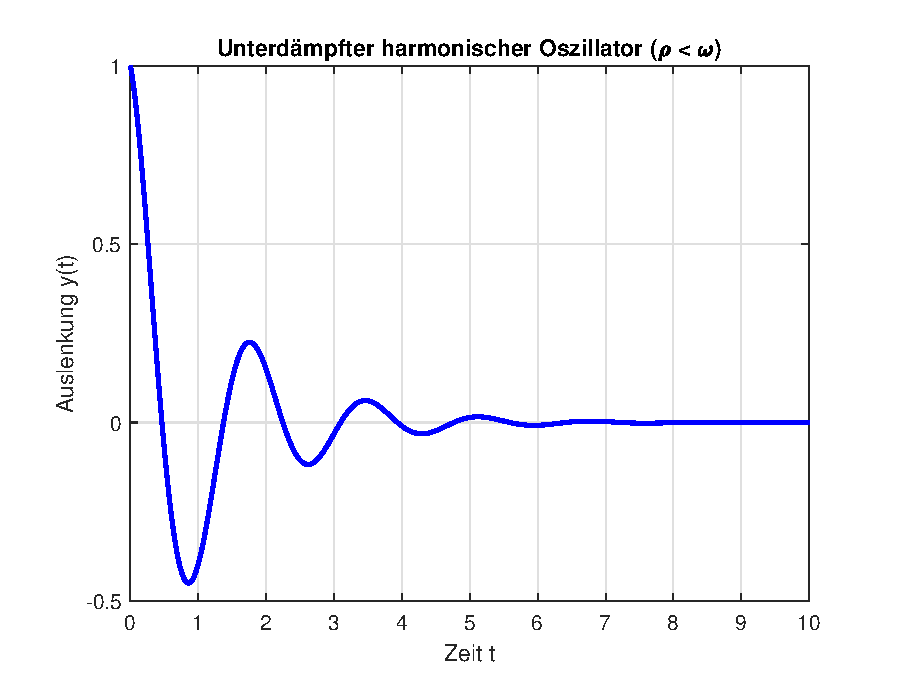
\includegraphics[width=0.3\textwidth]{unterdaempfterHarOszil.eps}
\end{figure}
}

\ErgebnisC{harmonischerOszillatorinhomogen}{
Fall 1: $y(t) = A\operatorname{e}^{(-\rho + \sqrt{\rho^2 - \omega^2})t} + B\operatorname{e}^{(-\rho - \sqrt{\rho^2 - \omega^2})t} + \frac{1}{2\sqrt{\rho^2 -\omega^2}}t \operatorname{e}^{(-\rho +  \sqrt{\rho^2 - \omega^2})t},$\\
Fall 2: $y(t) = (A+Bt) \operatorname{e}^{-\omega t} + \frac{1}{2}t^2 \operatorname{e}^{-\omega t},$\\
Fall 3: $y(t) = \operatorname{e}^{-\rho t}(A \cos(\sqrt{\omega^2 - \rho^2} t) + B \sin(\sqrt{\omega^2 - \rho^2} t))+\frac{1}{2}t\operatorname{e}^{-\rho t} \sin((\sqrt{\omega^2 - \rho^2})t).$
}




\ifthenelse{\boolean{mitLoes}}{\ruleBig \cleardoublepage}{}


%___________________________________________________________________
\newpage
\section*{Laplace-Transformation}
\addcontentsline{toc}{section}{Laplace-Transformation}
$f:[0,\infty) \rightarrow \mathbb{R}$ hei\ss t Laplace-transformierbar, wenn das Integral 
$$
F(s) := \mathcal{L}{f(t)} := \int_0^{\infty} \e^{-st} f(t) \mathrm{d}t \ \ \ f\"ur s \in \mathbb{R}
$$
existiert. Dabei ist $F(s)$ die Bildfunktion (auch Laplace-Transformierte genannt) zum Urbildfunktion $f(t)$. Hilfreich bei der Laplace-Transformation bzw. bei der R\"ucktransformation sind sogenannte Korrespondenztabellen, die zur Urbildfunktion die dazugeh\"orige Bildfunktion angeben.
\section*{Aufgaben zur Laplace-Transformation}
\addcontentsline{toc}{section}{Aufgaben zur Laplace-Transformation}
%30
\Aufgabe[e]{Laplace-Transformierte}
{
Berechnen Sie die Laplace-Transformierte von $f(t)=\sqrt{t}$: 
$$F(s):=\int\limits_0^\infty\EH{-st}\cdot\sqrt{t}\d t.$$
\textbf{ Hinweise}:
\begin{itemize}
\item Substituieren Sie $u=\sqrt t$. 
\item Spalten Sie $u^2$ in $u\cdot u$ auf und integrieren Sie partiell. 
\item Das Quadrat des verbleibenden Integrals k\"onnen Sie l\"osen, indem Sie Polarkoordinaten einführen.
\end{itemize}
}

\Loesung{
Mit der Substitution \ $u=\sqrt{t} \ \Rightarrow \ \text dt=2\,u\,\text du$ \ erhält man
	\[
	F(s) = \int\limits_{0}^{\infty} \EH{-s\,u^2}\cdot u\cdot 2\,u\ \text du = -\dfrac{1}{s}\cdot\int\limits_{0}^\infty  u\cdot(-2s u)\,\EH{-s\,u^2}\ \text du\ .
\]
Die partielle Integration ergibt
	\begin{align*}
	F(s) & = -\dfrac{1}{s}\left(u\EH{-s\,u^2}\Big|_0^\infty - \int\limits_{0}^\infty  
\EH{-s\,u^2}\ \text du\right)\\[1ex]
& =-\dfrac{1}{s}\left(0-0 - \int\limits_{0}^\infty  
\EH{-s\,u^2}\ \text du\right)\\[1ex]
&  = \dfrac{1}{s}\cdot\int\limits_{0}^\infty  \EH{-s\,u^2}\ \text du  \ .
\end{align*}
Mit Quadrieren erhält man
  \[
  \big(F(s)\big)^2 \ = \ \dfrac{1}{s}\,\int\limits_{0}^\infty \EH{-s\,x^2}\ \text dx 
                   \cdot \dfrac{1}{s}\,\int\limits_{0}^\infty \EH{-s\,y^2}\ \text dy \ = \ 
                   \dfrac{1}{s^2}\,\int\limits_{0}^\infty  \int\limits_{0}^\infty  \EH{-s\,(x^2+y^2)}\ \text dx\,\text dy 
\]
und durch Übergang zu Polarkoordinaten
  \[
  \big(F(s)\big)^2 \ = \ \dfrac{1}{s^2}\,\int\limits_{0}^\infty  \int\limits_{0}^{\pi/2} \EH{-s\,r^2}\ r\,\text d\phi\,\text dr \ = \
         \dfrac{1}{s^2}\cdot\dfrac{\pi}{2}\cdot \left[\frac{-1}{2\,s}\,\EH{-s\,r^2}\right]_0^\infty \ = \ \dfrac{\pi}{4\,s^3} \ .
\]
Damit ist 
\[
\ F(s) = {\cal L}\left(\sqrt{t}\right) = \sqrt{\dfrac{\pi}{4\,s^3}}\ .
\]
}



\ErgebnisC{AufglaplacTrafBere001}
{
$F(s)=\sqrt{\frac{\pi}{4s^3}}\,.$
}

\ifthenelse{\boolean{mitLoes}}{\ruleBig \cleardoublepage}{}
%31
\Aufgabe[e]{Laplace--Transformierte}
{
Bestimmen Sie unter Verwendung von ${\cal{L}}\big\{\sin(t)\big\} = \dfrac{1}{s^2+1}$  und geeigneten Rechenregeln folgende Ausdr\"ucke
	\[
	\textbf{a)} \ {\cal{L}}\left\{\frac{\sin(t)}{t}\right\}\ ,\quad
	\textbf{b)} \ {\cal{L}}\left\{\int\limits_0^t\frac{\sin(\tau)}{\tau}\ \text d\tau\right\}\ ,\quad
	\textbf{c)} \ \int\limits_{0}^{\infty}\frac{\sin(t)}{t}\ \text dt\ ,\quad
	\textbf{d)} \ {\cal{L}}\left\{\EH{-t}\,\frac{\sin(t)}{t}\right\}\ .
\]



%\textbf{e)} \ Bestimmen Sie \textbf{mit Hilfe des Faltungssatzes} der Laplace-Transformation die Urbildfunktion \  $f(t)$ \ zur Bildfunktion
%  \[
%  F(s) := \dfrac{s}{(s+1)(s^2+1)}\ .
%\]
}

\Loesung{
\begin{abc}
\item Mit der Transformationsformel \ \ ${\cal{L}}\left\{\dfrac{f(t)}{t}\right\} = \int\limits_{s}^\infty  F(\sigma)\ \text d\sigma$ \ \ erhält man
	\[
	{\cal{L}}\left\{\frac{\sin(t)}{t}\right\} = \int\limits_{s}^\infty  \dfrac{1}{\sigma^2+1}\ \text d\sigma = \Big[\arctan(\sigma)\Big]_s^\infty = \dfrac \pi2-\arctan(s)\ .
\]

\item\ Mit der Transformationsformel \ \ ${\cal{L}}\left\{\int\limits_{0}^{t} f(\tau) \text d\tau\right\} = \dfrac{F(s)}{s}$ \ \ erhält man 
	\[
	{\cal{L}}\left\{\int\limits_{0}^{t}\frac{\sin(\tau)}{\tau}\ \text d\tau\right\} = \frac 1s\cdot\left(\dfrac \pi2-\arctan(s) \right)
\]
%
%
\item

\textbf{1. Lösungsweg}\newline
Mit Hilfe des Anfangs- und Endwertsatzes ergibt sich 
\begin{align*}
\int\limits_{0}^\infty\frac{\sin(t)}{t}\, \mathrm{d}t
	   =& \lim_{t\to\infty} \int\limits_{0}^t\frac{\sin\tau}{\tau} \, \mathrm{d} \tau = \lim_{s\to 0}\left(
	   s\cdot {\cal{L}}\left\{\int\limits_{0}^t\frac{\sin(\tau)}{\tau} \, \mathrm{d} \tau\right\}\right) \\
=& \lim_{s\to 0}\left(\dfrac \pi2-\arctan(s) \right) = \dfrac \pi2\ .
\end{align*}

\textbf{2. Lösungsweg}\newline
Nach Definition der Laplace-Transformierten gilt
$${\cal{L}}\left\{\dfrac{\sin(t)}{t}\right\}=\int\limits_{0}^\infty\EH{-st}\cdot\frac{\sin(t)}{t}\ \text dt=U(s)$$

Aus der Teilaufgabe \textbf{a)} folgt $U(s)=\dfrac \pi2-\arctan(s)$.\newline
Somit erhält man
$$\int\limits_{0}^\infty\frac{\sin(t)}{t}\ \text dt=\int\limits_{0}^\infty\EH{-0\cdot t}\cdot\frac{\sin(t)}{t}\ \text dt=U(0)=\dfrac \pi2$$





\item Mit der Transformationsformel \ \ ${\cal{L}}\left\{\EH{-at}\,f(t)\right\} = F(s+a)$ \ \ erhält man
	\[
	{\cal{L}}\left\{\EH{-t}\,\frac{\sin(t)}{t}\right\} = \dfrac \pi2-\arctan(s+1)\ .
\]
\end{abc}

%%\textbf{e)} \ Es gilt
%$$
%F(s) = F_1(s) \cdot F_2(s) \quad \mbox{mit} \quad F_1(s) = \dfrac{1}{s+1}\,, \quad F_2(s)= \dfrac{s}{s^2+1}\,.
%$$
%Mit den Rücktransformierten 
%$$
%f_1(t) = \EH{-t} \quad \mbox{und} \quad f_2(t) = \cos( t)
%$$
%folgt
%\begin{align*}
%f(t) & = f_1(t) \ast f_2(t) = \int_0^t \EH{-(t-\tau)}\cos (\tau) \text d \tau = \EH{-t} \int_0^t \EH{\tau}\cos (\tau) \text d \tau\,.
%\end{align*}
%Mit 
%\begin{align*}
%I=&\int_0^t \EH{\tau}\cos \tau \text d \tau  = \EH{\tau}\sin \tau\Big|_0^t -  \int_0^t \EH{\tau}\sin \tau \text d \tau\\[1ex]
%& =  \EH{t}\sin t + \EH{\tau}\cos \tau |_0^t - \int_0^t \EH{\tau}\cos \tau \text d \tau\\[1ex]
%& =  \EH{t}\sin t + \EH{t}\cos t - 1  - I
%\end{align*}
%folgt
%$$2I=\EH{t}\sin t + \EH{t}\cos t - 1$$
%und
%$$
%I = \dfrac{1}{2}\,\EH{t}\sin t + \dfrac{1}{2}\,\EH{t}\cos t - \dfrac{1}{2}
%$$
%
%
%Alternativ kann man im Komplexen rechnen:
%\begin{align*}
%I=&\int_0^t \EH{\tau}\cos \tau \text d \tau  =\int_0^t \Real(\EH{\tau}\cdot\EH{i\tau})  \text d \tau \\[1ex]
%&=\Real\left(\int_0^t (\EH{(1+i)\tau}\text d \tau\right) =\left[\Real\left(\dfrac{\EH{(1+i)\tau}}{1+i}\right)\right]_0^t=\left[\EH{\tau}\Real\left(\dfrac{(\cos\tau+i\sin\tau)(1-i)}{2}\right)\right]_0^t\\[1ex]
%&=\left[\EH{\tau}\cdot\dfrac{(\cos\tau+\sin\tau)}{2}\right]_0^t=\EH{t}\cdot\dfrac{(\cos t+\sin t)}{2}-\dfrac{1}{2}\\
%\end{align*}
%
%Somit ergibt sich
%$$
%\ f(t) = \EH{-t} \cdot I=\dfrac{1}{2} (\sin t + \cos t) - \dfrac{1}{2}\,\EH{-t}\ .\ 
%$$

}

\ErgebnisC{AufglaplacTrafBere002}
{
\textbf{ a)} $F(s)=\frac \pi 2 - \arctan s$, 
\textbf{ b)} $F(s)=\frac {\pi/2-\arctan s} s$, 
\textbf{ c)} $F(s)=\frac \pi 2$,
\textbf{ d)} $F(s)=\frac \pi 2 - \arctan (s+1)$,
%\textbf{ e)} $\frac {\sin t + \cos t}2 - \frac{\EH{-t}}2$
}

\ifthenelse{\boolean{mitLoes}}{\ruleBig \cleardoublepage}{}
%32
\Aufgabe[e]{Laplace-Transformierte}
{
Berechnen Sie die Laplace-Transformierte der folgenden Funktionen: 
\begin{abc}
\item $f_1(t)=\left\{\begin{array}{ll}
A&\text{ f\"ur }0\leq t\leq t_0\\
A\EH{-2(t-t_0)}&\text{ sonst}
\end{array}\right.$ mit festem $A\in\R$. 
\item $f_2(t)=\left\{\begin{array}{ll}
0&\text{ f\"ur }0\leq t< a\\
A&\text{ f\"ur }a\leq t< b\\
0&\text{ sonst}
\end{array}\right.$ mit festen $0<a<b$ und $A\in\R$. 
\item $f_3(t)=\left\{\begin{array}{ll}
t&\text{ f\"ur }0\leq t\leq 3\\
3&\text{ f\"ur } t>3
\end{array}\right.$ 
\item $f_4(t)=\left\{\begin{array}{ll}
\sin t&\text{ f\"ur } t\leq \pi\\
0&\text{ f\"ur } t>\pi
\end{array}\right.$. 
\end{abc}
}

\Loesung{
\begin{abc}
\item \begin{align*}
\cL\{f_1(t)\}=& \int\limits_0^\infty \EH{-st}f_1(t)\d t = \int\limits_0^{t_0}\EH{-st}A \d t
+ \int\limits_{t_0}^\infty A\EH{-2(t-t_0)-st}\d t\\
=&\dfrac{A}{-s}\cdot\EH{-st}\Big|_0^{t_0}+\dfrac{A}{-s-2}\cdot\EH{(-s-2)t+2t_0}\Big|_{t_0}^{\infty}\\
=& \dfrac{A(1-\EH{-st_0})}{s} + \dfrac{A\EH{-st_0}}{2+s}=\dfrac As - \dfrac{2A\EH{-st_0}}{s^2+2s}
\end{align*}
\item $\cL\{f_2(t)\} =  \int\limits_a^bA\EH{-st}\d t = \dfrac{A(\EH {-as} - \EH {-bs})}{s}$
\item \begin{align*}
\cL\{f_3(t)\} =& \int\limits_0^3 t\EH{-st}\d t + \int\limits_3^\infty 3\EH{-st}\d t 
= \left. t\dfrac{\EH{-st}}{-s}\right|_0^3-\int\limits_0^3\dfrac{\EH{-st}}{-s}\d t
+ \left. \dfrac{3\EH{-st}}{-s}\right|_3^\infty\\
=& -\dfrac{3\EH{-3s}}s -\left. \dfrac{\EH{-st}}{s^2}\right|_0^3+\dfrac{3\EH{-3s}}{s}
= \dfrac{-\EH{-3s}+1}{s^2}
\end{align*}
\item 
\textbf{1.Lösungsweg:}(komplexe Zahlen)
\begin{align*}
&&\cL\{f_4(t)\} =& \int\limits_0^\pi\EH{-st}\sin t \d t \\
&& =& \int\limits_0^\pi\Imag(\EH{-st+it}) \d t\\
&&=&\Imag\left(\dfrac{\EH{-st+it}}{-s+i}\right)\Big|_0^\pi \\
&& =& \Imag\left(\dfrac{(-s-i)\EH{-st+it}}{s^2+1}\right)\Big|_0^\pi\\
&&= & \dfrac{\EH{-st}}{s^2+1}\cdot\Imag((-s-i)(\cos t+i\sin t))\Big|_0^\pi \\
&& =&\dfrac{\EH{-st}}{s^2+1}\cdot(-\cos t-s\sin t))\Big|_0^\pi \\
&&  =  & \frac {\EH{-s\pi}+1}{1+s^2}
\end{align*}

\textbf{2.Lösungsweg:} (zweifache partielle Integration)
\begin{align*}
&&\cL\{f_4(t)\} =& \int\limits_0^\pi\EH{-st}\sin t \d t 
= \bigl.-\cos t \EH{-st}\bigr|_0^\pi -\int\limits_0^\pi s\cos t \EH{-st}\d t \\
&&= & \EH{-s\pi}+1 - \bigl. s\sin t \EH{-st}\bigr|_0^\pi - \int\limits_0^\pi s^2\sin t \EH{-st}\d t \\
&&= & \EH{-s\pi}+1  - s^2\cdot\cL\{f_4(t)\} \\
\Rightarrow&& \cL\{f_4(t)\} =  & \frac {\EH{-s\pi}+1}{1+s^2}
\end{align*}
\end{abc}
}



\ErgebnisC{AufglaplacTrafBere003}
{
\textbf{ a)} $F_1(s)=\dfrac As - \frac{2A\EH{-st_0}}{s^2+2s}$, 
\textbf{ b)} $F_2(s)=\dfrac{A(\EH{-as}-\EH{-bs}}{s}$, 
\textbf{ c)} $F_3(s)=\dfrac{1-\EH{-3s}}{s^2}$, \\
\textbf{ d)} $F_4(s)=\dfrac{1+\EH{-s\pi}}{1+s^2}$
}

\ifthenelse{\boolean{mitLoes}}{\ruleBig \cleardoublepage}{}
%33
\Aufgabe[e]{Laplace-Transformierte}
{
\begin{abc}
\item Berechnen Sie die Laplace-Transformierte 
$$\mathcal{L}\{f(t)\}=F(s)=\int\limits_{t=0}^\infty \EH{-st}\cdot f(t)\d t$$ der folgenden Funktionen: 
\begin{iii}
\begin{multicols}{2}
\item $f(t) = 1$,
\item $f(t) = t$,
\item $f(t) = t^2$,
\item $f(t) = t^3$,
\item $f(t) = e^{-at}$,
\item $f(t) = e^{-at}\cdot t$,
\item ${\mathcal L}\{g'(t)\}$, f\"ur eine allgemeine (gegebene) Funktion $g(t)$,
\item ${\mathcal L}\{g''(t)\}$, f\"ur eine allgemeine (gegebene) Funktion $g(t)$.
\end{multicols}
\end{iii}
\textbf{Hinweis}: F\"ur die letzten beiden Aufgaben kann die Laplacetransformierte $G(s)=\sL\{g(t)\}$ der Funktion $g(t)$ als bekannt vorausgesetzt werden. 

\item Berechnen Sie die Laplace-Transformierte von $f(t)=\sqrt{t}$. \\
\end{abc}
\textbf{Hinweise}:
\begin{itemize}
\item Substituieren Sie $u=\sqrt t$. 
\item Spalten Sie $u^2$ in $u\cdot u$ auf und integrieren Sie partiell. 
\item Das Quadrat des verbleibenden Integrals k\"onnen Sie l\"osen, indem Sie Polarkoordinaten einführen.
\end{itemize}
}

\Loesung{
\begin{abc}
\item Diese Laplace-Transformationen müssen durch Anwendung der Definition und Bestimmung der Integrale berechnet werden. Es wird in der Regel partiell integriert. 
\begin{iii}
\item \begin{align*}
\mathcal{L}\{1\} =& \int\limits_{t=0}^\infty \EH{-st}1 \d t
= \left[\frac{\EH{-st}}{-s}\right]_{t=0}^\infty\\
=&  \dfrac{1}{s}
\end{align*}
\item \begin{align*}
\mathcal{L}\{t\} =& \int\limits_{t=0}^\infty \EH{-st}t \d t
= \left[t\frac{\EH{-st}}{-s}\right]_{t=0}^\infty+\frac 1 s\int\limits_{t=0}^\infty \EH{-st}\d t\\
=& 0 - \left.\frac{\EH{-st}}{-s^2}\right|_{t=0}^\infty
= \dfrac{1}{s^2}
\end{align*}
\item \begin{align*}
\mathcal{L}\{t^2\}  =& \int\limits_{t=0}^\infty t^2\EH{-st} \d t
= \left[t^2\frac{\EH{-st}}{-s}\right]_{t=0}^\infty+\frac 1 s \int\limits_{t=0}^\infty 2t\EH{-st}\d t\\
=& 0 + \left[\frac{2t\EH{-st}}{-s^2}\right]_{t=0}^\infty + \frac{2}{s^2}\int\limits_{t=0}^\infty \EH{-st}\d t\\
=&  0 +\left.\frac{2\EH{-st}}{-s^3}\right|_{t=0}^\infty= \dfrac{2}{s^3}
\end{align*}

\item \begin{align*}
\mathcal{L}\{t^3\}  =& \int\limits_{t=0}^\infty t^3\EH{-st} \d t
= \left[t^3\frac{\EH{-st}}{-s}\right]_{t=0}^\infty+\frac 1 s \int\limits_{t=0}^\infty 3t^2\EH{-st}\d t\\
=& 0 + \left[\frac{3t^2\EH{-st}}{-s^2}\right]_{t=0}^\infty + \frac{3}{s^2}\int\limits_{t=0}^\infty 2t\EH{-st}\d t\\
=&  0 +\left.\frac{6t\EH{-st}}{-s^3}\right|_{t=0}^\infty+\int\limits_{t=0}^\infty\frac{6\EH{-st}}{s^3}\d t\\
=& 0 + \left. \frac{6\EH{-st}}{s^4} \right|_{t=0}^\infty = \frac 6{s^4}
\end{align*}

\item \begin{align*}
\mathcal{L}\{\EH{-at}\} =& \int\limits_{t=0}^\infty \EH{-st}\EH{-at} \d t
= \left[\frac{\EH{-(s+a)t}}{-(s+a)}\right]_{t=0}^\infty\\
=&  \dfrac{1}{s+a}
\end{align*}

\item \begin{align*}
\mathcal{L}\{t\EH{-at}\} =& \int\limits_{t=0}^\infty t\EH{-at}\EH{-st} \d t
= \left[\frac{t\EH{-(s+a)t}}{-(s+a)}\right]_{t=0}^\infty+\frac 1{s+a}\int\limits_{t=0}^\infty \EH{-(s+a)t}\d t \\
=& 0 + \left.\frac{\EH{-(s+a)t}}{-(s+a)^2}\right|_{t=0}^\infty
=  \dfrac{1}{(s+a)^2}
\end{align*}

\item \begin{align*}
\mathcal{L}\{g'(t)\} =& \int\limits_{t=0}^\infty \EH{-st}g'(t) \d t\\
=& \left[\EH{-st}g(t)\right]_{t=0}^\infty - \int\limits_{t=0}^\infty(-s\EH{-st}g(t))\d t\\
=& 0-g(0)+s\mathcal{L}\{g(t)\}
= sG(s)-g(0)
\end{align*}

\item \begin{align*}
\mathcal{L}\{g''(t)\} =& \int\limits_{t=0}^\infty \EH{-st}g''(t) \d t\\
=&\left[\EH{-st}g'(t)\right]_{t=0}^\infty - \int\limits_{t=0}^\infty(-s\EH{-st}g'(t))\d t\\
=& 0-g'(0)+s\mathcal{L}\{g'(t)\}\\
=& s(sG(s)-g(0))-g'(0) = s^2G(s)-g'(0)-sg(0)
\end{align*}

\end{iii}

\item Mit der Substitution \ $u=\sqrt{t} \ \Rightarrow \ \text dt=2\,u\,\text du$ \ erhält man
	\[
	F(s) = \int\limits_{0}^{\infty} \EH{-s\,u^2}\cdot u\cdot 2\,u\ \text du = -\dfrac{1}{s}\cdot\int\limits_{0}^\infty  u\cdot(-2s u)\,\EH{-s\,u^2}\ \text du\ .
\]

Partielle Integration ergibt
	\begin{align*}
	F(s) & = -\dfrac{1}{s}\left(u\EH{-s\,u^2}\Big|_0^\infty - \int\limits_{0}^\infty  
\EH{-s\,u^2}\ \text du\right)\\[1ex]
& =-\dfrac{1}{s}\left(0-0 - \int\limits_{0}^\infty  
\EH{-s\,u^2}\ \text du\right)\\[1ex]
&  = \dfrac{1}{s}\cdot\int\limits_{0}^\infty  \EH{-s\,u^2}\ \text du  \ .
\end{align*}

Durch Quadrieren der Gleichung  erh\"alt man
  \[
  \big(F(s)\big)^2 \ = \ \dfrac{1}{s}\,\int\limits_{0}^\infty \EH{-s\,x^2}\ \text dx 
                   \cdot \dfrac{1}{s}\,\int\limits_{0}^\infty \EH{-s\,y^2}\ \text dy \ = \ 
                   \dfrac{1}{s^2}\,\int\limits_{0}^\infty  \int\limits_{0}^\infty  \EH{-s\,(x^2+y^2)}\ \text dx\,\text dy 
\]
und durch Übergang zu Polarkoordinaten
  \[
  \big(F(s)\big)^2 \ = \ \dfrac{1}{s^2}\,\int\limits_{0}^\infty  \int\limits_{0}^{\pi/2} \EH{-s\,r^2}\ r\,\text d\phi\,\text dr \ = \
         \dfrac{1}{s^2}\cdot\dfrac{\pi}{2}\cdot \left[\frac{-1}{2\,s}\,\EH{-s\,r^2}\right]_0^\infty \ = \ \dfrac{\pi}{4\,s^3} \ .
\]
Damit ist 
	\[
	 F(s) = {\cal L}\left(\sqrt{t}\right) = \sqrt{\dfrac{\pi}{4\,s^3}} .
\]
\end{abc}
}



\ErgebnisC{AufglaplacTrafBere01b}
{
\textbf{a)}\begin{multicols}{3}
\begin{iii}
\item $\dfrac{1}{s}$,
\item $\dfrac{1}{s^2}$,
\item $\dfrac{2}{s^3}$,
\item $\dfrac{3!}{t^4}$,
\item $\frac{1}{s+a}$,
\item $\dfrac{1}{(s+a)^2}$,
\item $ sG(s) - g(0)$,
\item $ s^2G(s) - sg(0) - g'(0)$.
\end{iii}
\end{multicols}
\textbf{b)}$F(s)=\sqrt{\frac{\pi}{4s^3}}\,.$
}

\ifthenelse{\boolean{mitLoes}}{\ruleBig \cleardoublepage}{}
%34
\Aufgabe[e]{Integralgleichungen mit Laplace--Transformation}
{
Bestimmen Sie die L\"osung $y(t)$ (mit \ $t\ge 0$) der Integralgleichung 
	\[
	y(t) = t^2 + \int\limits_{0}^{t} y(\tau)\,\sin(t-\tau)\ \text d\tau\,.
\]
}
\Loesung{
 Die Laplace--Transformation der Integralgleichung ergibt mit \ ${\cal L}\big(y(t)\big) = Y(s)$
 sowie
$$\int\limits_0^ty(\tau)\sin(t-\tau)\d \tau = \cL(y(t)*\sin(t))=\cL(y(t))\cdot \cL(\sin(t))$$
die Gleichung im Frequenzraum:
	\[
	\begin{array}{cl}
	& Y(s) = \dfrac{2}{s^3} + Y(s)\cdot\dfrac{1}{s^2+1}\\
	\\
	\Rightarrow & \left(1-\dfrac{1}{s^2+1}\right)\,Y(s) =\dfrac{2}{s^3} \,\Rightarrow\, Y(s) = \dfrac{2(s^2+1)}{s^3\cdot s^2} = \dfrac{2}{s^3}+\dfrac{2}{s^5} \\
	\\ 
	\Rightarrow & \underline{\underline{\ y(t) = t^2 + \dfrac{t^4}{12}\ }}\ .
	\end{array}
\]


}

\ErgebnisC{AufglaplacIntgGlgn001}
{
$y(t)=t^2+t^4/12$.
}

\ifthenelse{\boolean{mitLoes}}{\ruleBig \cleardoublepage}{}
%35
% \Aufgabe[f]{R\"ucktransformation}
% {
% Berechnen Sie
% \begin{align*}
% &\text{\bf a)}&&\, &\mathcal{L}^{-1}\left\{ \frac 5{s+2}\right\}&
% \qquad\qquad\text{\bf b)}& \, &\mathcal{L}^{-1}\left\{\frac {4s-3}{s^2+4}\right\}\\
% &\text{\bf c)}&&\, &\mathcal{L}^{-1}\left\{ \frac {2s-5}{s^2}\right\}&
% \qquad\qquad\text{\bf d)}& \, &\mathcal{L}^{-1}\left\{ \frac 1{s^2+2s}\right\}\\
% &\text{\bf e)}&&\, &\mathcal{L}^{-1}\left\{\frac {5s^2-15s+7}{(s+1)(s-2)^2}\right\}&
% \qquad\qquad\text{\bf f)}&\, &\mathcal{L}^{-1}\left\{\frac {4-5s}{s^{3/2}}\right\}.
% \end{align*}
% }
\Aufgabe[e]{Inverse Laplace-Transformation}
{
Bestimmen Sie
\begin{align*}
&\text{\textbf a)}&&\, &\mathcal{L}^{-1}\left\{ \frac 5{s+2}\right\}&
\qquad\qquad\text{\textbf b)}& \, &\mathcal{L}^{-1}\left\{\frac {4s-3}{s^2+4}\right\}\\
&\text{\textbf c)}&&\, &\mathcal{L}^{-1}\left\{ \frac {2s-5}{s^2}\right\}&
\qquad\qquad\text{\textbf d)}& \, &\mathcal{L}^{-1}\left\{ \frac 1{s^2+2s}\right\}\\
&\text{\textbf e)}&&\, &\mathcal{L}^{-1}\left\{\frac {5s^2-15s+7}{(s+1)(s-2)^2}\right\}&
\qquad\qquad\text{\textbf f)}&\, &\mathcal{L}^{-1}\left\{3\operatorname{e}^{-2s}\right\}\\
&\text{\textbf g)}&&\, &\mathcal{L}^{-1}\left\{ \frac{s}{(s+2)^2+9}\right\}&.
\end{align*}
}
\Loesung{
\begin{abc}
\item $$\mathcal{L}^{-1}\left\{ \dfrac 5 {s+2}\right\} = 5\mathcal{L}^{-1}\left\{\dfrac 1{s+2}\right\} = 5\operatorname{e}^{-2t}$$
\item \begin{align*}
\mathcal{L}^{-1}\left\{ \frac{4s-3}{s^2+4}\right\} 
=&  4 \mathcal{L}^{-1}\left\{\frac
s{s^2+2^2}\right\} - 3 \mathcal{L}^{-1}\left\{\frac 1 {s^2 + 2^2}\right\}\\
=& 4 \cos(2t)-\frac 32 \sin(2t)
\end{align*}
\item $$\mathcal{L}^{-1}\left\{\frac {2s-5}{s^2}\right\}
=2\mathcal{L}^{-1}\left\{\frac 1s\right\} - 5 \mathcal{L}^{-1}\left\{ \frac 1{s^2}\right\} 
= 2 - 5t$$
\item \begin{align*}
\mathcal{L}^{-1}\left\{ \frac 1{s^2+2s}\right\} = &\mathcal{L}^{-1}\left\{ \dfrac {\frac 12}s+ \dfrac {- \frac
12}{s+2}\right\}= \frac 12 \mathcal{L}^{-1}\left\{ \frac 1s\right\}- \frac
12 \mathcal{L}^{-1}\left\{ \frac 1{s+2}\right\}\\
=& \frac 12 - \frac 12 \operatorname{e}^{-2t}
\end{align*}
\item \begin{align*}
\mathcal{L}^{-1}\left\{\frac{5s^2-15s+7}{(s+1)(s-2)^2}\right\} = & 3 \mathcal{L}^{-1}\left\{ \frac 1 {s+1}\right\} +
2 \mathcal{L}^{-1}\left\{ \frac 1 {s-2}\right\} - \mathcal{L}^{-1}\left\{ \frac 1 {(s-2)^2}\right\}\\
=& 3\operatorname{e}^{-t} +2\operatorname{e}^{2t} - t\operatorname{e}^{2t}
\end{align*}
\item 
\begin{align*}
\mathcal{L}^{-1}\left\{3e^{-2s}\right\}=3\delta(t-2)
\end{align*}
\item
\begin{align*}
\mathcal{L}^{-1}\left\{ \frac{s}{(s+2)^2+9}\right\} 
&= \mathcal{L}^{-1}\left\{ \frac{s+2-2}{(s+2)^2+9}\right\} \\
&= \mathcal{L}^{-1}\left\{ \frac{s+2}{(s+2)^2+3^2}\right\}-2 \mathcal{L}^{-1}\left\{ \frac{1}{(s+2)^2+3^2}\right\} \\
&= e^{-2t} \cos(3t) - \frac{2}{3} e^{-2t} \sin(3t)
\end{align*}

%\begin{align*}
%\mathcal{L}^{-1}\left\{\frac{4-5s}{s^{3/2}}\right\}=&4\mathcal{L}^{-1}\left\{\frac{1}{s^{3/2}}\right\}-5 \mathcal{L}^{-1}\left\{\frac{1}{s^{1/2}}\right\}
%=4\mathcal{L}^{-1}\left\{\dfrac{\frac 1{\sqrt s}}{s}\right\} -5 \mathcal{L}^{-1}\left\{\frac{1}{\sqrt s}\right\}\\
%=&4\int_0^t\mathcal{L}^{-1}\left\{\frac{1}{\sqrt s}\right\}\text d t-5\dfrac1{\sqrt{\pi t}}
%=4\int_0^t\dfrac1{\sqrt{\pi t}}\text d t-5\dfrac1{\sqrt{\pi t}}\\
%=&\frac{4}{\sqrt{\pi}}\int_0^t t^{-\frac12}\text d t-5\dfrac1{\sqrt{\pi t}}
%= \frac{8\sqrt t }{\sqrt \pi} - \frac{5}{\sqrt{\pi t}}
%\end{align*}
%
%
%% Alternativ kann man die Formel
%% $$\mathcal{L}^{-1}\left\{\frac{1}{s^{a}}\right\}=\dfrac{t^{a-1}}{\Gamma(a)}$$
%% mit $\Gamma(\frac 12) = \sqrt \pi $ und $\Gamma(\frac 32)=\frac{\sqrt \pi}2$ benutzen.
%Alternatively, the formula
%$$\mathcal{L}^{-1}\left\{\frac{1}{s^{a}}\right\}=\dfrac{t^{a-1}}{\Gamma(a)}$$
%with $\Gamma(\frac 12) = \sqrt \pi $ and $\Gamma(\frac 32)=\frac{\sqrt \pi}2$ can be used.
\end{abc}
}



\ErgebnisC{AufglaplacTrafBere004}
{
{\textbf a)} $5\operatorname{e}^{-2t}                                             $
{\textbf b)} $4 \cos(2t)-\frac 32 \sin(2t)                          $
{\textbf c)} $ 2 - 5t                                               $
{\textbf d)} $\frac 12 - \frac 12 \operatorname{e}^{-2t}                          $
{\textbf e)} $3\operatorname{e}^{-t} +2\operatorname{e}^{2t} - t\operatorname{e}^{2t}                         $
{\textbf f)} $\frac{8\sqrt t }{\sqrt \pi} - \frac{5}{\sqrt{\pi t}}  $

}









\ifthenelse{\boolean{mitLoes}}{\ruleBig \cleardoublepage}{}
%36
\Aufgabe[e]{Laplace transform}
{
Answer the following points giving and example if necessary:
\begin{iii}
\item How is the Laplace transform defined?
\item Why the variable $s$ has to be positive?
\item What is the Heaviside function $h_{t_0}(t)$?
\item Explain with an example what is the damping of a function $f(t)$.
\item Is it true that $\mathcal{L}\left\{f(t)+g(t)\right\} = F(s)+G(s)$?
\item Is it true that $\mathcal{L}\left\{f(t)\,g(t)\right\} = F(s)\,G(s)$?
\item Recapitulate how to solve an initial value problem using the Laplace transform.
\item Write the properties of the Dirac delta function $\delta(t)$ (also called $\delta$-distribution).
\end{iii}
}


\Loesung{
\begin{iii}
\item How is the Laplace transform defined?

$\mathcal{L}\left\{f(t)\right\} = \int_0^\infty \operatorname{e}^{-st} f(t) \d t$.

\item Why the variable $s$ has to be positive?

Because the upper limit of the integral in the definition of the Laplace transform is $\infty$ and the exponential function $\operatorname{e}^{-st}$ is bounded for $t\rightarrow \infty$ only if $s>0$.
\item What is the Heaviside function $h_{t_0}(t)$?

It is the step function that is 0 for $t<t_0$ and 1 for $t\geq t_0$.
\item Explain with an example what is the damping of a function $f(t)$.

Show the graph of $\operatorname{e}^{-t} f(t)$ with $f(t)=\dfrac{t}{10}$ or $f(t)=\sin(t)$.

\begin{tikzpicture}
    \begin{axis}[
     axis lines=middle,clip=false,
            xmin=-1,xmax=10, ymin=-0.5,ymax=0.5,
            xticklabel style={black},
            xlabel=$x$,
            ylabel=$y$]
    \addplot[domain=0:10,samples=200,red]{exp(-x)*x}
				node[draw, above,pos=1.3,font=\footnotesize]{$f(x)=\operatorname{e}^{-t}\, \frac{t}{10}$};
    \addplot[domain=0.5:10,samples=200,blue]{exp(-x)}
				node[left,pos=0,font=\footnotesize]{$f(x)=\operatorname{e}^{-t}$};
    \addplot[domain=0:5,samples=200,cyan]{x/10}
				node[right,pos=1.,font=\footnotesize]{$f(x)=\dfrac{t}{10}$};
    \end{axis}
  \end{tikzpicture}

\begin{tikzpicture}
    \begin{axis}[
     axis lines=middle,clip=false,
            xmin=-1,xmax=6.28, ymin=-0.5,ymax=2,
            xticklabel style={black},
            xlabel=$x$,
            ylabel=$y$]
    \addplot[domain=0:6.28,samples=200,red]{exp(-x)*sin(deg(x))}
				node[right, draw,pos=1.1,font=\footnotesize]{$f(x)=\operatorname{e}^{-t}\, \sin(t)$};
    \addplot[domain=-0.5:6.28,samples=200,blue]{exp(-x)}
				node[left,pos=0,font=\footnotesize]{$f(x)=\operatorname{e}^{-t}$};
    \addplot[domain=0:6.28,samples=200,cyan]{sin(deg(x))}
				node[above,pos=0.3,font=\footnotesize]{$f(x)=\sin(x)$};
    \end{axis}
  \end{tikzpicture}

\item Is it true that $\mathcal{L}\left\{f(t)+g(t)\right\} = F(s)+G(s)$? YES.

\item Is it true that $\mathcal{L}\left\{f(t)\,g(t)\right\} = F(s)\,G(s)$? NO

\item Recapitulate how to solve an initial value problem using the Laplace transform.

\renewcommand{\labelenumi}{\arabic{enumi}}
 \setcounter{enumi}{0}
\begin{enumerate}
\item Transform right and left hand side of the ODE: Apply $\mathcal{L}\{\cdot\}$.
\item Substitute the initial values and solve for $Y(s)$.
\item Inverse transform (use the table) left and right hand side of the equation to get $y(t)=\mathcal{L}^{-1}(Y(s))$.
\end{enumerate}

\item Write the properties of the Dirac delta function $\delta(t)$ (also called $\delta$-distribution).

\begin{align*}
&\int_{-\infty}^\infty \delta(t) \d t = 1, \\
&\int_{-\infty}^\infty \delta(t-a) \d t = 1, \quad \text{ (arbitrary } a)\\
&\int_{-\infty}^\infty \delta(t-t_0)\, f(t) \d t = f(t_0)\\
\end{align*}

\end{iii}

}




\ifthenelse{\boolean{mitLoes}}{\ruleBig \cleardoublepage}{}
%37
\Aufgabe[e]{Heaviside-Funktion}
{
Gesucht ist die Laplace--Transformierte von
$$
	f(t) := h(t-2)\cdot t^2 \ ,
$$
wobei \ $h$ \ die Heaviside--Funktion ist.

\begin{abc}
\item Mit Hilfe der Integraldarstellung der Definition.

\item Mit Hilfe des Verschiebungssatzes und der Tabelle der Laplace--Transformierten.
\end{abc}
}

\Loesung{
\textbf{a)}
	\[
	F(s) = \int\limits_{2}^{\infty} \EH{-s\,t}\,t^2\ \text dt = \left[-\left(\frac{t^2}{s}+\frac{2\,t}{s^2}+\frac{2}{s^3}\right)\cdot\EH{-s\,t}\right]_2^\infty = \left(\frac{4}{s}+\frac{4}{s^2}+\frac{2}{s^3}\right)\cdot\EH{-2\,s}\ .
\]
\noindent
\textbf{b)} \ Für den Verschiebungssatz
	\[
	{\cal{L}}\Big( f(t-a)\cdot h(t-a)\Big) = F(s)\cdot\EH{-a\,s}\ ,\ \ a>0\ ,
\]
 muss die Funktion erst umgeschrieben werden:
	\[
	t^2 = (t-2)^2+4(t-2)+4 \ .
\]
Damit erhält man die Laplace--Transformierte
	\[
	{\cal{L}}\Big(\big( (t-2)^2+4(t-2)+4\big)\cdot h(t-2)\Big) = \left(\frac{2}{s^3}+\frac{4}{s^2}+\frac{4}{s}\right)\cdot\EH{-2\,s}
\]
}

\ErgebnisC{laplacTranHeav001}{
$F(s)= \left(\frac{2}{s^3}+\frac{4}{s^2}+\frac{4}{s}\right)\cdot\EH{-2\,s}$
}

\ifthenelse{\boolean{mitLoes}}{\ruleBig \cleardoublepage}{}
%38
\Aufgabe[e]{Verschiebungssatz}
{
\begin{abc}
\item Berechnen Sie die Laplace-Transformation der Funktion \( f(t) = h(t-3) e^{t-3} \).
\item Berechnen Sie die Inverse Laplace-Transformation von \(\frac{1}{(s-2)^2}\).
\item Berechnen Sie die Inverse Laplace-Transformation von \(\frac{1}{(s-1)^2} e^{-3s}\).
\end{abc}

}

\Loesung{

\textbf{Lösung zu a):}

1. Nutzen Sie die Verschiebungseigenschaft der Laplace-Transformation:
   Wenn \( \mathcal{L}\{f(t)\} = F(s) \), dann gilt \( \mathcal{L}\{f(t-a)h(t-a)\} = e^{-as}F(s) \).

   In diesem Fall ist \( f(t-a) = e^{t-a} \). Bei $a=3$ ist $e^{t-3}$. 

2. Finden Sie die Laplace-Transformation von \( e^t \) (nicht von $e^{t-3}$):
   \[
   \mathcal{L}\{e^t\} = \int_0^\infty e^{t} e^{-st} dt = \int_0^\infty e^{(1-s)t} dt
   \]
   Damit das Integral konvergiert, muss \( s > 1 \) sein:
   \[
   \mathcal{L}\{e^t\} = \frac{1}{s-1}
   \]

3. Wenden Sie die Verschiebungseigenschaft an:
   \[
   \mathcal{L}\{e^{t-3}h(t-3)\} = e^{-3s} \cdot \mathcal{L}\{e^t\} = e^{-3s} \cdot \frac{1}{s-1}
   \]


\textbf{Lösung zu b):}
1. Die allgemeine Formel für die Inverse Laplace-Transformation von \(\frac{1}{(s-a)^n}\) ist:
   \[
   \mathcal{L}^{-1}\left\{\frac{1}{(s-a)^n}\right\} = \frac{t^{n-1} e^{at}}{(n-1)!}
   \]

2. Für unseren speziellen Fall ist \( a = 2 \) und \( n = 2 \).

   Mit der Formel erhalten wir:
   \[
   \mathcal{L}^{-1}\left\{\frac{1}{(s-2)^2}\right\} = \frac{t^{2-1} e^{2t}}{(2-1)!} = \frac{t e^{2t}}{1} = t e^{2t}
   \]



\textbf{Lösung zu c):}

1. Identifizieren Sie die Verschiebungseigenschaft:
   Der Term \( e^{-3s} \) deutet auf eine Zeitverschiebung in der ursprünglichen Funktion hin. Speziell gilt, wenn \( \mathcal{L}\{f(t)\} = F(s) \), dann ist \( \mathcal{L}\{f(t-a)h(t-a)\} = e^{-as}F(s) \).

2. Finden Sie die Inverse Laplace-Transformation der unverschobenen Funktion:
   Betrachten Sie \(\frac{1}{(s-1)^2}\). Wir erkennen, dass die Inverse Laplace-Transformation von \(\frac{1}{(s-a)^2}\) \( t e^{at} \) ist:
   \[
   \mathcal{L}^{-1}\left\{\frac{1}{(s-1)^2}\right\} = t e^{t}
   \]

3. Wenden Sie die Verschiebungseigenschaft an:
   Der Term \( e^{-3s} \) zeigt eine Verschiebung um 3 Einheiten an. Daher:
   \[
   \mathcal{L}^{-1}\left\{\frac{1}{(s-1)^2} e^{-3s}\right\} = (t-3) e^{(t-3)} h(t-3)
   \]
}
\ErgebnisC{AufglaplaceVerschiebung001}
{
\begin{abc}
\item
\[
\mathcal{L}\{ h(t-3) e^{t-3} \} = \frac{e^{-3s}}{s-1}
\]
\item
\[
\mathcal{L}^{-1}\left\{\frac{1}{(s-2)^2}\right\} = t e^{2t}
\]
\item
\[
\mathcal{L}^{-1}\left\{\frac{1}{(s-1)^2} e^{-3s}\right\} = (t-3) e^{(t-3)} h(t-3)
\]
\end{abc}


}

\ifthenelse{\boolean{mitLoes}}{\ruleBig \cleardoublepage}{}
%39
\Aufgabe[e]{LR-Kreis mit Hilfe der Laplace-Transformation}
{
Ein Stromkreis habe einen Widerstand von \ $R=0.8$ Ohm \ und eine Selbstinduktion von \ $L=4$ Henry\,. Bis zur Zeit \ $t_0=0$ \ fließe kein Strom. Dann wird eine Spannung von \ $U=5$ Volt \ angelegt. Nach $5$ Sekunden wird
die Spannung abgeschaltet. Gesucht ist der Stromverlauf \
$I(t)$ \ für \ $0 \le t \le 5$ \ und \ $t > 5$. 
%\begin{abc}
%\item Ermitteln  Sie $I(t)$ als L\"osung eines Anfangswertproblems. \\
%\textbf{Hinweis}: L\"osen Sie \textit{ zwei } Anfangswertprobleme, wobei Sie den Anfangswert $I(5)$ des zweiten AWP als Funktionswert der L\"osung des ersten AWP erhalten.
%\item
Ermitteln Sie $I(t)$ mit Hilfe der Laplace-Transformation. 
%\end{abc} 

\textbf{Hinweis}: In diesem Stromkreis gilt $L\dot I(t) + RI(t)=U(t)$ mit
$$U(t)=5\cdot(1-h(t-5))=\left\{\begin{array}{ll}
5,&0\leq t\leq 5\\
0,& t>5
\end{array}.\right.$$
mit der Heaviside-Funktion $h(t)$. 
}

\Loesung{
%\begin{enumerate}\renewcommand{\labelenumi}{\textbf{\alph{enumi})}}
%\item Es gilt die Differentialgleichung
%\[
%  L\dot{I}(t)+RI(t)=U(t)
%\]
%
%Die L\"osung der homogenen Gleichung $L\dot I_h(t)+RI_h(t)=0$ ergibt sich durch% Einsetzen des Exponentialansatzes
%$$I_h(t)=A\EH{\lambda t} \text{ mit } \dot I_h(t)=\lambda\cdot A\EH{\lambda t}:$$
%\begin{align*}
%&&L\lambda\cdot A \EH{\lambda t} + R A\EH{\lambda t}=& 0\\
%\Rightarrow && L\lambda + R=& 0&\text{ f\"ur } A\neq 0\\
%\Rightarrow && \lambda=& - \frac{R}L=-\frac 15.
%\end{align*}
%Es m\"ussen nun beide Anfangswertprobleme betrachtet werden: 
%\begin{itemize}
%\item $0\leq t\leq 5$: Inhomogene Differentialgleichung $L\dot I(t)+RI(t)=5$ mit $I(0)=0$. \\
%Eine Partikul\"arl\"osung der inhomogenen Differentialgleichung ist 
%$$I_p(t)=\frac 5 R= \frac{5}{0.8}=\frac{25}4, $$
%denn damit gilt $L\dot I_p(t)+RI_p(t)=0 + R\frac{5}R=5.$\\
%Die allgemeine L\"osung der inhomogenen Differentialgleichung ist die Summe der Partikul\"arl\"osung der inhomogenen Gleichung und der allgemeinen L\"osung der homogenen Gleichung: 
%$$I_{\text{allg},1}(t)= I_h(t)+I_p(t) = A_1\EH{\lambda t} + \frac{25}4.$$
%Eingesetzt in die Anfangsbedingung $I(0)=0$ ergibt sich damit
%\begin{align*}
%&&A_1\EH{0} + \frac {25}4 = & 0 \qquad \Rightarrow A_1=-\frac{25}4.
%\end{align*}
%\item $t>5$: Das zweite Anfangswertproblem ist bereits homogen, hat also die L\"osung 
%$$I_{\text{allg},2}(t)=A_2\EH{\lambda t}.$$
%Die Anfangsbedingung ergibt sich mit Hilfe der L\"osung des ersten AWP zu 
%\begin{align*}
%&&I_{\text{allg}, 1}(5)=-\frac{25}4\EH{\lambda \cdot 5}+\frac{25}4 \overset!=& I_{\text{allg},2}(5)=A_2\EH{\lambda\cdot 5}\\
%\Rightarrow&& A_2=& -\frac{25}4 + \frac{25}4\EH{-5\lambda} = \frac{25}4\left( \EH{-5\lambda}-1\right)=\frac{25}4\left(\EH{ }-1\right)
%\end{align*}
%\end{itemize}
%Das Zusammentragen beider L\"osungen f\"uhrt dann auf 
%$$I_{AWP}(t)=\frac{25}4\cdot \left\{\begin{array}{ll}
%(1-\EH{-t/5}), & 0\leq t \leq 5\\
%(\EH{ }-1)\EH{-t/5}, & t>5
%\end{array}\right.$$
%Anmerkung: F\"ur die Rechnung wurde auf die Angabe der physikalischer Einheiten verzichtet. Da alle Gr\"oßen in SI-Einheiten gegeben waren, sind auch die Ergebnisse in SI-Einheiten, die Stromst\"arke ist hier also in Ampere gegeben. \\
%Dieser Stromverlauf ist im folgenden skizziert: 
%\item
%%%%%%%%%
Es sei $Y(s)$ die Laplace-Transformierte des Stroms $I(t)$. Damit gilt
\begin{align*}
&& \sL\{L\dot I(t)+RI(t)\}=& \sL\{U(t)\}\\
\Rightarrow&& L (sY(s)-\underbrace{I(0)}_{=0})+ R Y(s) =& 5\cdot \sL\{1-h(t-5)\}\\
&&=& 5\left( \frac 1s - \frac{\EH{-5s}}s\right)\\
\end{align*}
Diese (algebraische) Gleichung hat die L\"osung
$Y(s)=\dfrac{5(1-\EH{-5s})}{s(sL+R)}=\dfrac{25(1-\EH{-5s})}{4s(5s+1)}$. \\
Vor der eigentlichen R\"ucktransformation betrachten wir zun\"achst
\begin{align*}
\frac 1{s(5s+1)} = & \frac{1}s-\frac{5}{5s+1}
=& \mathcal{L}\left\{  1 - \EH{-t/5}\right\}
\end{align*}
Daraus ergibt sich dann 
\begin{align*}
I(s)=& \frac{25}4\sL^{-1}\left\{\frac{1-\EH{-5s}}{s(5s+1)}\right\}\\
=& \frac{25}4\left( 1-\EH{-t/5} - \left(1-\EH{-(t-5)/5}\right)h(t-5)\right)\\
=&\frac{25}4\cdot \left\{\begin{array}{ll}
(1-\EH{-t/5}), & 0\leq t \leq 5\\
(\EH{ }-1)\EH{-t/5}, & t>5
\end{array}\right.. 
\end{align*}

%\end{enumerate}
\begin{center}
\psset{xunit=.5cm}
\begin{pspicture}(-1,-2)(20,8)
\psgrid[subgriddiv=0, gridcolor=lightgray](-1,-1)(20,8)
\psline{->}(-1,0)(20,0)
\psline{->}(0,-1)(0,8)
\put(9.5,-.4){$t/s$}
\put(.2,7.6){$I/A$}
\psplot[plotpoints=100, plotstyle=curve, linecolor=lightgray]
{0}{20}
{
25 4 div 1 2.7183 x -.2 mul exp neg add mul
}
\psplot[plotpoints=100, plotstyle=curve]
{0}{5}
{
25 4 div 1 2.7183 x -.2 mul exp neg add mul
}

\psplot[plotpoints=100, plotstyle=curve]
{5}{20}
{
25 4 div 2.7183 -1 add 2.7183 x -.2 mul exp mul mul 
}

\psline[linestyle=dashed, linecolor=lightgray](0,6.25)(20,6.25)
\put(-.4,6.2){$\frac{25}4$}
\end{pspicture}
\end{center}
Dieser Stromverlauf ist plausibel. W\"urde die Spannung bei $5V$ bleiben, w\"urde sich asymptotisch (f\"ur $t\to\infty$) eine Stromst\"arke von $I=\frac {25}4A$ einstellen (graue Kurve). Stattdessen f\"allt der Strom nach f\"unf Sekunden exponentiell ab und wird f\"ur $t\to\infty$ ganz verschwinden. 

}

\ErgebnisC{gewdglStrmLrkr01c}
{
$$I(t)=\frac{25}4\cdot \left\{\begin{array}{ll}
(1-\EH{-t/5}), & 0\leq t \leq 5\\
(\EH{ }-1)\EH{-t/5}, & t>5
\end{array}\right.$$
}

\ifthenelse{\boolean{mitLoes}}{\ruleBig \cleardoublepage}{}
%40
\Aufgabe[e]{Anfangswertprobleme zu linearen Differentialgleichungen $n$-ter Ordnung}
{
Gegeben seien die folgenden Anfangswertprobleme: 
\begin{abc}
\item $y^{\prime\prime}(t) - 2 y^\prime(t) - 3y(t) = 4 \EH{t}, \quad y(0) = 0, 
         \quad y'(0) = 6,$
\item $y^{\prime\prime}(t)+4y^\prime(t)+4y(t)=4 \EH{-2t}, \quad y(0)=1 ,\quad
  y^\prime(0)=0$.
\end{abc}
Bestimmen Sie die L\"osungen jeweils mit Hilfe des Exponentialansatzes \textbf{und} zus\"atzlich mit Hilfe der Laplace-Transformation. 
}

\Loesung{
Zun\"achst die L\"osung mittels Exponentialansatz: \\
\begin{abc}
\item Die Nullstellen des charakteristischen Polynoms
$p(\lambda)=\lambda^2-2\lambda-3$ sind $\lambda_1=-1$ und $\lambda_2=3$. 
Eine Partikul\"arl\"osung der inhomogenen Gleichung berechnet man mit
dem Ansatz $y_p(t)=ae^t$, es folgt
$ -4 a e^t \stackrel{!}{=}4e^t$ und damit $a=-1$. Die allgemeine L\"osung
ist 
$$ y_{allg}(t) = - e^t + c_1 \EH{-t} + c_2 \EH{3t} \ \text{ mit } c_1,c_2 \in \R .$$
Aus den Anfangsbedingungen $y(0)=-1+c_1+c_2 \stackrel{!}{=} 0$
und $y^\prime(0) = -1 - c_1 + 3c_2 \stackrel{!}{=} 6$ folgt das lineare 
Gleichungssystem
$$ \begin{array}{rcrl}
   c_1 & + & c_2 & = 1, \\
   -c_1 & + & 3c_2 & = 7 
   \end{array} $$
mit L\"osung $c_2=2$ und $c_1=-1$. Damit ist 
$$ y_{AWP}(t) = -e^t-\EH{-t}+2\EH{3t}. $$

\item Die Nullstelle von $p(\lambda)=\lambda^2+4\lambda+4$ ist
$\lambda=-2$, dies ist eine doppelte Nullstelle. Als Ansatz f\"ur die
Partikul\"arl\"osung muss man 
$y_p(t)=at^2 \EH{-2t}$ nehmen, denn man hat Resonanz der Ordnung 2. 
Mit $y_p^\prime(t) = a \EH{-2t} \big( 2t-2t^2\big)$
und $y_p^{\prime\prime}(t) = a \EH{-2t} \big(2-8t+4t^2\big)$
folgt
$2a \EH{-2t} \stackrel{!}{=} 4 \EH{-2t}$ und damit $a=2$. 
Dies liefert die allgemeine L\"osung
$$ y_{allg}(t) = \big( 2t^2 + c_1 t + c_2 \big) \EH{-2t}
   \ \text{ mit } c_1,c_2 \in \R. $$
Die Anfangsbedingungen  $y(0)=c_2 \stackrel{!}{=} 1$ und
$y^\prime(0) = c_1-2c_2 \stackrel{!}{=} 0$ liefern $c_2=1$ und $c_1=2$ 
und damit die L\"osung
$$ y_{AWP}(t) = \big( 2t^2 + 2t + 1 \big) \EH{-2t} . $$ 
\end{abc}
Nun die L\"osung mit Hilfe der Laplace-Transformation: 
\begin{abc}
\item Die Laplace-Transformation der Differentialgleichung ergibt
\begin{align*}
&&\sL\{4\EH{t}\}=&\sL\{y''(t)-2y'(t)-3y(t)\}\\
\Rightarrow&&\frac{4}{s-1}=&s^2Y(s)-y'(0)-sy(0)-2(sY(s)-y(0))-3Y(s)\\
&&=&s^2Y(s)-6-2sY(s)-3Y(s)
\end{align*}
Die L\"osung im Bildbereich ist dann
\begin{align*}
Y(s)=&\frac 1{s^2-2s-3}\cdot \left( \frac 4{s-1}+6\right)\\
=& \frac{6s-2}{(s-1)(s-3)(s+1)}
\end{align*}
Diese l\"asst sich mittels Partialbruchzerlegung darstellen als 
\begin{align*}
Y(s)=& \frac{-1}{s-1} + \frac{2}{s-3} + \frac{-1}{s+1}
\end{align*}
und die R\"ucktransformation ergibt die L\"osung des Anfangswertproblems: 
\begin{align*}
y(t)=& -\sL^{-1}\left\{\frac{1}{s-1}\right\} + 2 \sL^{-1}\left\{\frac 1{s-3}\right\} -\sL^{-1}\left\{\frac 1{s+1}\right\}\\
=& - \EH{t} + 2 \EH{3t}-\EH{-t}
\end{align*}
\item Die Laplace-Transformation der Differentialgleichung ergibt
\begin{align*}
&&\sL\{4\EH{-2t}\}=&\sL\{y''(t)+4y'(t)+4y(t)\}\\
\Rightarrow&&\frac{4}{s+2}=&s^2Y(s)-y'(0)-sy(0)+4(sY(s)-y(0))+4Y(s)\\
&&=&s^2Y(s)-s+4sY(s)-4+4Y(s)
\end{align*}
Die L\"osung im Bildbereich ist dann
\begin{align*}
Y(s)=&\frac 1{s^2+4s+4}\cdot \left( \frac 4{s+2}+s+4\right)\\
=& \frac{s^2+6s+12}{(s+2)^3}
\end{align*}
Diese l\"asst sich mittels Partialbruchzerlegung darstellen als 
\begin{align*}
Y(s)=& \frac{1}{s+2} + \frac{2}{(s+2)^2} + \frac{4}{(s+2)^3}
\end{align*}
und die R\"ucktransformation ergibt die L\"osung des Anfangswertproblems: 
\begin{align*}
y(t)=& \EH{-2t}+2t\EH{-2t}+4\frac{t^2\EH{-2t}}{2}
= \EH{-2t}(1+2t+2t^2)
\end{align*}
\end{abc}
 
}


\ErgebnisC{gewdglLineAWPr001}
{
a) $y(t) = -e^t-\EH{-t}+2\EH{3t}$\\
b) $y(t) = \big( 2t^2 + 2t + 1 \big) \EH{-2t}$
}

\ifthenelse{\boolean{mitLoes}}{\ruleBig \cleardoublepage}{}
%41
% \Aufgabe[e]{Lineare Differentialgleichung}
% {
% Gegeben sei das Anfangswertproblem für \ $u(t)$
% $$	u'' + 4\,u' +3\,u = 12\cdot\Big(1-h(t-2)\Big)\ ,\quad u(0)=u'(0)=0$$
% wobei \ $h(t)$ \ die Heaviside--Funktion ist.


% \textbf{a)} \ Bestimmen Sie die Lösung mit Hilfe der Laplace--Transformation.

% \textbf{b)} \ Geben Sie die Lösung in den Bereichen  $0\le t < 2$  und  $ 2\le t$ ohne Verwendung der Heaviside--Funktion an und fassen Sie die Terme sinnvoll zusammen.

% }
\Aufgabe[e]{Linear ODE}
{
Gegeben sie das folgende Anfangswertproblem für $y(t)$ durch
$$	y'' + 4\,y = t\ ,\quad y(0)= 1, y'(0)=2.$$

\textbf{a)} \ Berechnen Sie die Lösung mit dem Exponentialansatz.

\textbf{b)} \ Berechnen Sie die Lösung mit Hilfe der Laplace-Transformation.

}

\Loesung{
\textbf{a)} 
Die allgemeine Lösung ist gegeben durch die Lösung des homogenenen Systems und der 
partikulären Lösung
% The solution is given by the solution of the homogeneous system plus a particular solution
$$y(t) = y_h(t) + y_p(t).$$
Für das homogene System betrachten wir die Nullstellen des charakteristischen Polynoms
% For the homogeneous system we consider the zeros of the characteristic polynomial
$$\lambda^2+4=0,$$
welche die komplex Konjugierten sind
% which are the complex conjugates
$$\lambda = \pm 2\operatorname{i}.$$
Daher ist die Lösung des homogenen Systems
% Therefore, the solution of the homogeneous system is
$$y_h(t) = C_1 \cos{2t} + C_2 \sin{2t}.$$
Die beiden Konstanten werden mit den Anfangswerten bestimmt.
% The two constants will be determined with the initial conditions.

Für die partikuläre Lösung machen wir den Ansatz
% For the particular solution we make the ansatz
$$y_p(t) = A_0 + A_1 t,$$
weil die rechte Seite der Differentialgleichung ein lineares Polynom ist.
% because the right hand side of the differential equation is a linear polynomial.
Die beiden Konstanten $A_0$ und $A_1$ werden durch einsetzen in deiGleichung bestimmt.
% The two constants $A_0$ and $A_1$ are determined inserting the solution in the equation.
Da $y'=A_1$ und $y''=0$, erhalten wir
$$4(A_0+A_1t) = t$$
und mit Koeffizientenvergleich gilt
% and the coefficients comparison gives 
$$A_0=0, \qquad A_1 = \frac{1}{4}.$$
Insgesamt ergibt sich die allgemeine Lösung
$$y(t) = \frac{1}{4}t + C_1 \cos{2t} + C_2 \sin{2t}.$$
Aus den Anfangswerten erhalten wir
$$y(0) = C_1 = 1$$
und 
$$y'(0)= \frac{1}{4} + 2C_2 \stackrel{!}{=} 2 \rightarrow C_2 = \frac{7}{8}.$$
Die spezielle Lösung ist dann
% The solution is
$$y(t) = \frac{1}{4}t+\cos{2t} + \frac{7}{8}\sin{2t}.$$

\textbf{b)}
Mit der Laplace-Transformation gilt
% With the Laplace transform it is
$$s^2Y(s) -s-2+4Y(s) = \frac{1}{s^2}$$
$$(s^2+4)Y(s) = \frac{1}{s^2}+s+2$$
$$Y(s) = \frac{s^3+2s^2+1}{s^2(s^2+4)}$$
Partialbruchzerlegung
$$\frac{s^3+2s^2+1}{s^2(s^2+4)}= \frac{A}{s}+ \frac{B}{s^2} + \frac{Cs+D}{s^2+4}$$
Multiplikation beider Seiten mit $s^2(s^2+4)$ 
$$s^3+2s^2+1= As(s^2+4)+ B(s^2+4) + (Cs+D)s^2$$
der Wert $s=0$ führt zu $B=\frac{1}{4}$.
$$s^3+2s^2+1= As^3+4As+ \frac{1}{4}s^2+1 + Cs^3+Ds^2$$
Mit Koeffizientenvergleich erhalten wir
\begin{align*}
A&=0\\
C&=1\\
D+\frac{1}{4}&=2 \quad \rightarrow \quad D=\frac{7}{4}
\end{align*}
$$Y(s) = \frac{1}{4}\cL^{-1}\left\{ \frac{1}{s^2} \right\} + \cL^{-1}\left\{ \frac{s}{s^2+2^2} \right\} + \frac{7}{4}\frac{1}{2}\cL^{-1}\left\{ \frac{2}{s^2+2^2} \right\}$$
$$y(t) = \frac{1}{4}t + \cos{2t} + \frac{7}{8}\sin{2t}.$$

}

%\newcounter{AufglaplacldglKlLp001}
%\setcounter{AufglaplacldglKlLp001}{\theAufg}
%\Ergebnis{\subsubsection*{Ergebnisse zu Aufgabe \arabic{Blatt}.\arabic{AufglaplacldglKlLp001}:}
%
%}

\ifthenelse{\boolean{mitLoes}}{\ruleBig \cleardoublepage}{}
%42
% \Aufgabe[f]{AWP mit Laplace--Transformation}
% {
% Bestimmen Sie mit Hilfe der Laplace--Transformation die Lösung der Anfangswertaufgabe: 
% $$ u''(t)+4\,u'(t)-12\,u(t)=4\,\text{e}^{-2\,t}$$
% mit den Anfangswerten 
% $$u(0)=0 \text{ und }  u'(0)=0\;.$$
% %&  &  &  &  &  &  \\ 
% %\mathbf{ii)} &  & v''(t)+25\,v(t)=80\,\sin (3\,t) & , & v(0)=3
% %& , & v'(0)=5\;. \\ 
% %&  &  &  &  &  &  \\ 
% %\mathbf{iii)} &  & w''(t)+25\,w(t)=50\,\sin (5\,t) & , & 
% %w(0)=1 & , & w'(0)=5\;. \\ 
% %&  &  &  &  &  &  \\ 
% %\mathbf{iv)} &  & x''(t)+4\,x'(t)+13\,x(t)=0 & , & 
% %x(0)=6 & , & x'(0)=0\;.

% }
\Aufgabe[e]{IVP with Laplace transform}
{
Compute the solution of the following initial value problem using the Laplace transform:
$$ u''(t)+4\,u'(t)-12\,u(t)=4\,\text{e}^{-2\,t}$$
with the initial values
$$u(0)=0 \text{ and }  u'(0)=0\;.$$
%&  &  &  &  &  &  \\ 
%\mathbf{ii)} &  & v''(t)+25\,v(t)=80\,\sin (3\,t) & , & v(0)=3
%& , & v'(0)=5\;. \\ 
%&  &  &  &  &  &  \\ 
%\mathbf{iii)} &  & w''(t)+25\,w(t)=50\,\sin (5\,t) & , & 
%w(0)=1 & , & w'(0)=5\;. \\ 
%&  &  &  &  &  &  \\ 
%\mathbf{iv)} &  & x''(t)+4\,x'(t)+13\,x(t)=0 & , & 
%x(0)=6 & , & x'(0)=0\;.

}
\Loesung{
%\textbf{i)\ \ }
% Die Laplace--Transformation der AWA lautet mit\ \ $%
% u_{0}=u_{0}'=0$\ : 
% \begin{align*}
% &  & \left( s^{2}\,U(s)-s\,u_{0}-u_{0}'\right) +4\cdot \left(
% s\,U(s)-u_{0}\right) -12\cdot U(s)\;=\;\dfrac{4}{s+2} \\ 
% &  &  \\ 
% \Rightarrow &  & \left( s^{2}+4\,s-12\right) \cdot U(s)\;=\;\dfrac{4}{s+2}
% \\ 
% &  &  \\ 
% \Rightarrow &  & U(s)\;=\;\dfrac{4}{\left( s+2\right) \,\left(
% s^{2}+4\,s-12\right) }\;=\;\dfrac{\frac{-1}{4}}{s+2}+\dfrac{\frac{1}{8}}{s-2}%
% +\dfrac{\frac{1}{8}}{s+6}
% \end{align*}
% Die Rücktransformation ergibt die Lösung der AWA\thinspace : 
% \[
% u_{\text{AW}}(t)=\dfrac{-1}{4}\,\text{e}^{-2\,t}+\dfrac{1}{8}\,\text{e}%
% ^{2\,t}+\dfrac{1}{8}\,\text{e}^{-6\,t}\;\;. 
% \]
With $%
u_{0}=u_{0}'=0$, the Laplace transform of the IVP reads:
\begin{align*}
&  & \left( s^{2}\,U(s)-s\,u_{0}-u_{0}'\right) +4\cdot \left(
s\,U(s)-u_{0}\right) -12\cdot U(s)\;=\;\dfrac{4}{s+2} \\ 
&  &  \\ 
\Rightarrow &  & \left( s^{2}+4\,s-12\right) \cdot U(s)\;=\;\dfrac{4}{s+2}
\\ 
&  &  \\ 
\Rightarrow &  & U(s)\;=\;\dfrac{4}{\left( s+2\right) \,\left(
s^{2}+4\,s-12\right) }\;=\;\dfrac{\frac{-1}{4}}{s+2}+\dfrac{\frac{1}{8}}{s-2}%
+\dfrac{\frac{1}{8}}{s+6}
\end{align*}
Resubstitution yields the solution of the IVP\thinspace : 
\[
u_{\text{AW}}(t)=\dfrac{-1}{4}\,\text{e}^{-2\,t}+\dfrac{1}{8}\,\text{e}%
^{2\,t}+\dfrac{1}{8}\,\text{e}^{-6\,t}\;\;. 
\]

%\begin{align*}
%\mathbf{ii)} &  & v_{\text{AW}}(t)=5\,\sin (3\,t)-2\,\sin (5\,t)+3\,\cos
%(5\,t)\;\;. \\ 
%&  &  \\ 
%\mathbf{iii)} &  & w_{\text{AW}}(t)=-5\,t\,\cos (5\,t)+2\,\sin (5\,t)+\cos
%(5\,t)\;\;. \\ 
%&  &  \\ 
%\mathbf{iv)} &  & x_{\text{AW}}(t)=\,\text{e}^{-2\,t}\cdot \big(4\,\sin
%(3\,t)+6\,\cos (3\,t)\big)\;\;.
%\end{align*}
}

\ErgebnisC{AufglaplacAnfwAufg001}
{
$u_{\text{AW}}(t)=\dfrac{-1}{4}\,\text{e}^{-2\,t}+\dfrac{1}{8}\,\text{e}^{2\,t}+\dfrac{1}{8}\,\text{e}^{-6\,t}$
}

\ifthenelse{\boolean{mitLoes}}{\ruleBig \cleardoublepage}{}
%43
\Aufgabe[e]{AWP mit Laplace--Transformation}
{
Bestimmen Sie mit Hilfe der Laplace--Transformation die Lösung der Anfangswertaufgabe: 
$$ y''(t)-3\,y'(t)+2\,y(t)=4\,\text{e}^{2\,t}$$
mit den Anfangswerten 
$$y(0)= -3 \text{ und }  y'(0)=5\;.$$
}

\Loesung{
% \textbf{i)\ \ }
Die Laplace--Transformation der AWP lautet mit\ \ $%
y_{0}= -3, , y_{0}'=5$\ : 
\begin{align*}
&  & \left( s^{2}\,Y(s)-s\,y_{0}-y_{0}'\right) -3\cdot \left(
s\,Y(s)-y_{0}\right) +2\cdot Y(s)\;=\;\dfrac{4}{s-2} \\ 
&  &  \\ 
\Rightarrow &  & \left( s^{2}\,Y(s)+3s-5\right) -3\cdot \left(
s\,Y(s)+3\right) +2\cdot Y(s)\;=\;\dfrac{4}{s-2} \\ 
&  &  \\ 
\Rightarrow &  & \left( s^{2}-3\,s+2\right) \cdot Y(s)\;=\;\dfrac{4}{s-2}-3s+14
\\ 
&  &  \\ 
\Rightarrow &  & Y(s)\;=\;\dfrac{4+(14-3s)(s-2)}{\left( s-2\right) \,\left(
s^{2}-3\,s+2\right) }\;=\;\dfrac{-3s^2+20s-24}{(s-2)(s-2)(s-1)}.
\end{align*}

Durchf\"uhren einer Partialbruchzerlegung:
\begin{align*}
\dfrac{-3s^2+20s-24}{(s-2)(s-2)(s-1)} &= \dfrac{A}{s-2} + \dfrac{B}{(s-2)^2} + \dfrac{C}{s-1} \\
-3s^2+20s-24 &= A(s-2)(s-1) + B(s-1) + C(s-2)^2
\end{align*}
Der Wert $s=1$ f\"uhrt zu $C = -7$, der Wert $s=2$ f\"uhrt zu $B = 4$. Ein Koeffizientenvergleich ergibt $A=4$.
Damit gilt:
$$
Y(s) = \dfrac{4}{s-2} + \dfrac{4}{(s-2)^2} - \dfrac{7}{s-1}
$$

Die Rücktransformation ergibt die Lösung der AWP\thinspace : 
\[
y_{\text{AW}}(t)= 4\,\text{e}^{2\,t}+ 4 t\,\text{e}%
^{2\,t}-7\,\text{e}^{t};. 
\]
}

\ErgebnisC{AufglaplacAnfwAufg002}
{
$u_{\text{AW}}(t)=\dfrac{-1}{4}\,\text{e}^{-2\,t}+\dfrac{1}{8}\,\text{e}^{2\,t}+\dfrac{1}{8}\,\text{e}^{-6\,t}$
}

\ifthenelse{\boolean{mitLoes}}{\ruleBig \cleardoublepage}{}
%44
\Aufgabe[e]{Balkenbiegung}
{
Ein homogener Balken ($E,J$\ konstant) der Länge \ $L=3$ \ möge an beiden Enden gelenkig gelagert sein. Bei 2/3 der Länge greife eine
punktförmige Last \ $F$ \ an. Berechnen Sie die Lage des tiefsten Punktes des Balkens, wobei sein
Eigengewicht vernachlässigt werden darf.\\
Das Materialgesetz des Balkens wird als
\[
EJ\cdot w''''(x)=-F\cdot \delta (x-l) \qquad (\text{mit }l=\frac 23 L)
\]
angenommen. \\
\textbf{Hinweise}: $EJ$ bezeichnet die Biegesteifigkeit des Balkens. Zur Vereinfachung k\"onnen Sie annehmen $EJ=1$. Ebenson k\"onnen Sie $F=1$ setzen. \\
Gehen Sie in den folgenden Schritten vor: 
\begin{abc}
\item Ermitteln Sie die L\"osung $w_H(x)$ der homogenen Differentialgleichung. 
\item Bestimmen Sie  eine spezielle Lösung $w_P(x)$ (bzw. $W_P(s)$) der inhomogenen Differentialgleichung, indem Sie die
Laplace-Transformation nutzen, wobei Sie von
homogenen Anfangswerten ausgehen k\"onnen. 
\item Bestimmen Sie die Integrationskonstanten der allgemeinen L\"osung der inhomogenen Gleichung
$w(x)=w_H(x)+w_P(x)$ aus den Randbedingungen 
$$w(0)=w(L)=0\qquad \text{ und }\qquad w''(0)=w''(L)=0.$$
\item Berechnen Sie den Extremwert der so erhaltenen Funktion. 
\end{abc}
}
\Loesung{
Wir vereinfachen die Differentialgleichung zu 
$$w^{(4)}(x)=-6\alpha \delta(x-l)$$
mit der neuen Konstanten $\alpha=\frac{F}{6EJ}$. 
\begin{abc}
\item Die homogene Gleichung $w_H^{(4)}(x)=0$ kann durch einfache Integration gel\"ost werden: 
$$w_H(x)=A+Bx+Cx^2+Dx^3.$$
\item 
Für \ \ $w_P(0)=w_P'(0)=w_P''(0)=w_P'''(0)=0$ \ \ lautet die Laplace--Transformation der inhomogenen
linearen Differentialgleichung \ \ $w_P^{(4)}(x)=-6\alpha\cdot \delta (x-l)\;:$
\[
s^4\;W_P(s)=-6\alpha\cdot \,\text{e}^{-l\,s} \,\Rightarrow\, W_P(s)=-6\alpha\cdot \frac{\text{e}^{-l\,s}}{s^4}\;. 
\]

Die Rücktransformation ergibt 
\[
w_{P}(x)=-6\alpha\cdot \frac{(x-l)^3}6\cdot h(x-l)=-\alpha(x-l)^3\cdot h(x-l)\;. 
\]
Dabei ist $h(x)=\left\{\begin{array}{rr}0&\text{ f\"ur }x<0\\ 1&\text{ f\"ur }x\geq
0\end{array}\right.$ die Heaviside-Funktion. 
\item 
Damit lautet die allgemeine Lösung: 
\[
w(x)=w_H(x)+w_P(x)=A+B\,x+C\,x^2+D\,x^3-\alpha \,(x-l)^3\cdot h(x-l). 
\]

Die Randbedingungen ergeben: 
\[
\begin{array}{rcllll}
w(0) = 0 & : &  & A=0 &  &  \\ 
&  &  &  &  &  \\ 
w''(0)= 0 & : &  & 2\,C=0 &  &  \\ 
&  &  &  &  &  \\ 
w(L) = 0 & : &  & B\cdot L + D\cdot L^3 - \alpha (L-l)^3  = 0 \\
&  &  &  &  &  \\ 
w''(L) = 0 & : &  & 6\cdot D \cdot L -6\,\alpha (L-l)= 0 \\
\end{array}
\]
In den letzen beiden Zeilen wurde $A=C=0$ ber\"ucksichtigt. \\
Aus der letzten erh\"alt man 
$$D=\frac{\alpha(L-l)}{L}=\frac{\alpha }{3}$$
und damit aus der dritten:
$$B=\frac{\alpha(L-l)^3-DL^3}{L}=\frac{\alpha\frac{L^3}{27}- \frac{\alpha}3L^3}L = \frac{-8\alpha L^2}{27}.$$
Insgesamt haben wir so als L\"osung der Randwertaufgabe: 
\begin{align*}
w(x)=&-\frac{8\alpha}{27}L^2x + \frac{\alpha}3 x^3- \alpha(x-l)^3\cdot h(x-l)\\
=& -\frac 83 \alpha x + \frac \alpha 3 x^3 - \alpha(x-2)^3\cdot h(x-2).
\end{align*}
\item Das Minimum dieser Funktion liegt entweder in einem station\"aren Punkt ($w'(x)=0$) oder an
den R\"andern des Definitionsbereichs ($x=0$, $x=3$) oder an der Sprungstelle der
Funktionsdefinition ($x=2$). Dort ist die Funktion zwar zweimal differenzierbar, aber auf die
Berechnung der Ableitung wird hier verzichtet. Die station\"aren Punkte in den Teilintervallen
$[0,2]$ und $[2,3]$ ergeben sich zu: 
\begin{iii}
\item $0< x<2 $: 
\begin{align*}
&&0=& w'(x)= -\frac 8 3 \alpha +\alpha x^2&
\Rightarrow && x=& \sqrt{\frac 83} 
\end{align*}
Die negative Wurzel entf\"allt wegen der Bedingung $0<x$. 
\item $2<x<3$:
\begin{align*} 
&&0=& w'(x)= -\frac 8 3 \alpha +\alpha x^2 -3\alpha (x-2)^2\\
\Rightarrow && 0=& (1-3)x^2+12x-12-\frac 83 \\
\Rightarrow && 0=& x^2-6x+\frac{22}3=\left( x- 3\right)^2- 9 + \frac{22}3\\
\Rightarrow&&  x=&3\pm\sqrt{\frac 53}
\end{align*}
Beide L\"osungen liegen außerhalb des betrachteten Definitionsintervalls $(2<x<3)$
\end{iii}
Kandidaten f\"ur das Minimum sind also $x_1=0,\, x_2=\sqrt{8/3},\, x_3=2,\, x_4=3$ 
mit 
$$w(0)=0,\, w(x_2)=-\frac 23 x_2^3\alpha< w(2)=-\frac 83\alpha,\, w(3)=0.$$
Damit liegt das Minimum bei $x_2=\sqrt{\frac 83}$. 
\end{abc}
\begin{center}
\begin{pspicture}(-1,-3)(4,.4)
\psgrid[gridcolor=lightgray,linecolor=lightgray](-1,-3)(4,0)
\psplot[plotpoints=100, plotstyle=curve, linecolor=black]
{0}{2}
{
-8 27 div 9 mul x mul x 3 exp 3 div add 
}
\psplot[plotpoints=100, plotstyle=curve]
{2}{3}
{
-8 27 div 9 mul x mul x 3 exp 3 div add x -2 add 3 exp neg add
}
\psline[linewidth=2pt]{->}(2,-1)(2,-2.666)
\end{pspicture}
\end{center}
}
\ErgebnisC{AufglaplacBalkBieg001}
{
$w_P(x)=-\frac{F}{6EJ}(x-l)^3\cdot h(x-l)$, $x_{\text{min}}=\sqrt{\frac 8{27}}L$
}

\ifthenelse{\boolean{mitLoes}}{\ruleBig \cleardoublepage}{}
%45
\Aufgabe[]{}{
Gegeben sei das Anfangswertproblem
%$$u''(t)-2u'(t)+u(t)=t+\cos(t)\cdot h(t-\pi)$$
$$u''(t)-2u'(t)+u(t)=\cos(t)\cdot h(t-\pi)$$
mit $u(0)=0$ und $u'(0)=0$. Dabei ist $h(t)$ die Heaviside-Funktion. 
\begin{abc}
\item Zeigen Sie, dass die L\"osung des Anfangswertproblems im Bildbereich der Laplace-Transformation die folgende Gestalt hat:
%$$U(s)=\left( \frac 1{s^2} - \frac{s}{1+s^2}\EH{-s\pi}\right) \frac 1{(s-1)^2}$$
$$U(s)=- \frac{s\, \EH{-s\pi}}{(1+s^2)(s-1)^2}$$
\item Bestimmen Sie die L\"osung der Differentialgleichung $u(t)$ im Urbildbereich.
\end{abc}
}
\Loesung{
\begin{abc}
\item Die Laplace-Transformierte des Anfangswertproblems ist
%$$s^2U(s)-2sU(s)+U(s)=\frac 1{s^2}+\sL\{\cos(t)\cdot h(t-\pi)\}.$$
$$s^2U(s)-2sU(s)+U(s)=\sL\{\cos(t)\cdot h(t-\pi)\}.$$
F\"ur die Transformation des letzten Terms wird der Verschiebungssatz angewendet:
\begin{align*}
\sL\{\cos(t)\cdot h(t-\pi)\}=&\sL\{\cos(t-\pi+\pi)\cdot h(t-\pi)\}=\sL\{\cos(t+\pi)\}\EH{-s\pi}\\
=& \sL\{-\cos(t)\}\EH{-s\pi}=\frac{-s}{1+s^2}\EH{-s\pi}.
\end{align*}
Damit ist die transformierte Differentialgleichung:
%$$U(s)(s^2-2s+1)=\frac 1{s^2}-\frac{s}{1+s^2}\EH{-s\pi}.$$
$$U(s)(s^2-2s+1)=-\frac{s}{1+s^2}\EH{-s\pi}.$$
Die L\"osung im Bildbereich ist
%$$U(s)=\frac 1{(s-1)^2}\left( \frac 1{s^2}-\frac{s}{1+s^2}\EH{-s\pi}\right).$$
$$U(s)=-\frac{s}{(1+s^2)(s-1)^2}\EH{-s\pi}.$$
\item Die R\"ucktransformation ergibt
%\begin{align*}
%u(t)=&\sL^{-1}\left\{\frac 1{(s-1)^2s^2}\right\} - \sL^{-1}\left\{\frac{s}{(s-1)^2(1+s^2)}\EH{-s\pi}\right\}\\
%\end{align*}
\begin{align*}
u(t)=& - \sL^{-1}\left\{\frac{s}{(s-1)^2(1+s^2)}\EH{-s\pi}\right\}
\end{align*}
%Die Partialbruchzerlegung der beiden Terme ergibt
%\begin{align*}
%&&\frac 1{(s-1)^2s^2}=& \frac{A  }{s-1} + \frac{ B }{(s-1)^2} + \frac{C  }{s}+\frac{D  }{s^2}\\
%&&=& \frac{(A+C)s^3+(-A+B-2C+D)s^2+(C-2D)s+D}{(s-1)^2s^2}\\
%\Rightarrow&&A+C=&0,\, -A+B-2C+D=0,\, C-2D=0,\, D=1\\
%\Rightarrow&&D=&1,\, C=2,\, A=-2,\, B=A+2C-D=1
%\end{align*}
%und
Die Partialbruchzerlegung des Bruches ergibt
\begin{align*}
&&&\frac{s}{(s-1)^2(1+s^2)}\\
&&=& \frac{E}{s-1}+\frac{F}{(s-1)^2}+\frac{G+Hs}{1+s^2}\\
&&=& \frac{(E+H)s^3+(-E+F+G-2H)s^2+(E-2G+H)s-E+F+G}{(s-1)^2(1+s^2)}\\
\Rightarrow&&E+H=&0,\, -E+F+G-2H=0,\, E-2G+H=1,\, -E+F+G=0\\
\Rightarrow&&H=&0,\, E=0,\, G=-\frac 12,\, F=\frac 12
\end{align*}
Damit ist dann
\begin{align*}
u(t)=&%\sL^{-1}\left\{ \frac{-2}{s-1}+\frac 1{(s-1)^2}+\frac 2{s}+\frac 1{s^2}\right\} + 
-\frac 12 \sL^{-1}\left\{ \left( \frac 1 {(s-1)^2}-\frac 1{1+s^2}\right)\EH{-\pi s}\right\}\\
=& %-2\EH t + t\EH t+2 +t + 
-\frac 12 \left[t\EH t-\sin(t)\right]_{t\leftarrow t-\pi}h(t-\pi)\qquad\text{ (Verschiebungssatz)}\\
=&% (t-2)\EH t + 2 + t +
 -\frac 12\left[ (t-\pi)\EH{t-\pi}-\sin(t-\pi)\right] h(t-\pi)\\
=& %(t-2)\EH t + 2+t + 
-\frac 12\left[ (t-\pi)\EH{t-\pi}+\sin(t)\right]h(t-\pi)\\
=&\left\{\begin{array}{ll}
0&\text{ f\"ur } t\leq \pi\\
-\frac{1}2\left[(t-\pi)\EH{t-\pi}+\sin(t)\right]&\text{ f\"ur } t>\pi.
\end{array}\right.
\end{align*}

\end{abc}
}





\ifthenelse{\boolean{mitLoes}}{\ruleBig \cleardoublepage}{}
%46
\Aufgabe[e]{Lineare Differentialgleichung}
{
Gegeben sei das Anfangswertproblem für \ $u(t)$
$$	u'' + 4\,u' +3\,u = 12\cdot\Big(1-h(t-2)\Big)\ ,\quad u(0)=u'(0)=0$$
wobei \ $h(t)$ \ die Heaviside--Funktion ist.

\begin{abc}
\item Bestimmen Sie die Lösung mit Hilfe der Laplace--Transformation.

\item Geben Sie die Lösung in den Bereichen  $0\le t < 2$  und  $ 2\le t$ ohne Verwendung der Heaviside--Funktion an und fassen Sie die Terme sinnvoll zusammen.
\end{abc}
}

\Loesung{
\begin{abc}
\item Die Laplace--Transformation des AWPs ergibt
	\[
	s^2\,U(s) +4s\,U(s)+3\,U(s) = \frac{12}{s}\cdot\Big(1-\EH{-2s}\Big)\ .
\]
Die Laplace--Transformierte der Lösung ergibt sich damit zu
	\[
	U(s) = \frac{12}{s\cdot(s+3)\cdot(s+1)}\cdot\Big(1-\EH{-2s}\Big) = \left(\frac 4s + \frac{2}{s+3} + \frac{-6}{s+1}\right) \cdot\Big(1-\EH{-2s}\Big)\ .
\]

Die Rücktransformation ergibt die gesuchte Lösung
	\[
	u(t) = 4+2\,\EH{-3\,t}-6\,\EH{-t} - h(t-2)\cdot\Big(4+2\,\EH{-3\,(t-2)}-6\,\EH{-(t-2)}\Big) \ .
\]

\item	\[
	u(t) = \left\{\begin{array}{ccl}
	       4+2\,\EH{-3\,t}-6\,\EH{-t} & \text{für} & 0\le t < 2 \\
	       \\
	       \left(2-2\,\EH6\right)\cdot \EH{-3\,t} + \left(-6+6\,\EH2\right)\cdot\EH{-t} & \text{für} & 2\le t
	       \end{array}\right.\ .
\]
\end{abc}
\psset{xunit=1cm, yunit=1cm, runit=1cm}
\begin{pspicture}(-1,-1)(5,4)
\psgrid[subgriddiv=1,griddots=10,gridlabels=.3](0,0)(5,4)
\psline{-}(2,0)(2,4)
\psplot[plotpoints=200, plotstyle=curve]
{0}{2}
{
4 2 2.72 3 neg x mul exp mul add 6 neg 2.72 x neg exp mul add
}

\psplot[plotpoints=200, plotstyle=curve]
{2}{5}
{ 
2 2 neg 2.72 6 exp mul add 2.72 3 neg x mul exp mul 6 neg 6 2.72 2 exp mul add 2.72 x neg exp mul add
}

\end{pspicture}

}

\ErgebnisC{AufglaplacldglKlLp001}{
\begin{abc}
\item $u(t) = 4+2\,\EH{-3\,t}-6\,\EH{-t} - h(t-2)\cdot\Big(4+2\,\EH{-3\,(t-2)}-6\,\EH{-(t-2)}\Big)$
\item $u(t) = \left\{\begin{array}{ccl}
	       4+2\,\EH{-3\,t}-6\,\EH{-t} & \text{für} & 0\le t < 2 \\
	       \\
	       \left(2-2\,\EH6\right)\cdot \EH{-3\,t} + \left(-6+6\,\EH2\right)\cdot\EH{-t} & \text{für} & 2\le t
	       \end{array}\right.\ $
\end{abc}
}

\ifthenelse{\boolean{mitLoes}}{\ruleBig \cleardoublepage}{}
%47
\Aufgabe[e]{Lineare Differentialgleichung}
{
Gegeben sei das Anfangswertproblem für \ $u(t)$
$$	u'' +\,u = \sin(t)\cdot\Big(1-h(t-\pi)\Big)\ ,\quad u(0)=u'(0)=0$$
wobei \ $h(t)$ \ die Heaviside--Funktion ist.

\begin{abc}
\item Bestimmen Sie zun\"achst die L\"osung im Bereich $0 \leq t \leq \pi$ mit Hilfe des Exponentialansatzes und dann die L\"osung im Bereich $t \geq \pi$.

\item Bestimmen Sie die L\"osung des AWPs mit Hilfe der Laplace-Transformation
\end{abc}
}

\Loesung{
\begin{abc}
\item Im Bereich $0 \leq t \leq \pi$ gilt f\"ur die homogene lin. Dgl. $u''(t)+u(t)=0$. Das charakteristische Polynom
$$
\lambda^2+1=0
$$
besitzt die Nullstellen $\lambda_{1,2} = \pm i$. Daraus folgt die allgemeine homogene L\"osung
$$
u_{\text{h}}(t) = a \sin(t) + b \cos(t), \, a,b \in \mathbb{R}.
$$
F\"ur die partikul\"are L\"osung w\"ahlen wir den Ansatz
$$
u_{\text{p}}(t) = A t \sin(t) + B t \cos(t).
$$
Bilden der Ableitungen
\begin{align*}
u_{\text{p}}'(t)  &= (A-Bt)\sin(t) +(At+B)\cos(t) \\
u_{\text{p}}''(t) &= (2A-Bt)\cos(t) -(At+2B)\sin(t)
\end{align*}
und einsetzen in die Dgl. $u''(t)+u(t)=\sin(t)$ liefert
$$
2A\cos(t) -2B\sin(t) = \sin(t).
$$
Damit ergibt sich $A=0$ und $B= -1/2$. Damit folgt
$$
u_{\text{p}}(t) = - \frac{1}{2}t \cos(t)
$$
und damit die allgemeine L\"osung 
$$
u(t) = a \sin(t) + b \cos(t) - \frac{1}{2}t \cos(t), \, a,b \in \mathbb{R}.
$$
Mit den Anfangswertbedingungen
\begin{align*}
u(0) &= 0 = a \sin(0) +b \cos(0) \Rightarrow b = 0\\
u'(0) &= a \cos(0) -b\sin(0)-\frac{1}{2} \cos(0) +\frac{1}{2}\cdot 0 \cdot \sin(0) \Rightarrow a = \frac{1}{2}
\end{align*}
ergibt sich die L\"osung des AWPs
$$
u_{\text{AWP}}(t) = \frac{1}{2} \sin(t) -\frac{1}{2} t\cos(t), \, 0\leq t \leq \pi.
$$

\noindent
Am Endes des Bereiches bei $t=\pi$ gilt:
$$
u_{\text{AWP}}(\pi) = \frac{\pi}{2} \, \text{und} \, u_{\text{AWP}}'(\pi) = 0.
$$
Dies sind die Anfangswerte f\"ur den zweiten Bereich. Im zweiten Bereich ist die lin. Dgl. homogen mit der schon bekannten allg. L\"osung
$$
u(t)= a \sin(t) +b \cos(t) \Rightarrow  u_{\text{AWP}}(t) = - \frac{\pi}{2} \cos(t), \, t \geq \pi.
$$

\item 
F\"ur den Verschiebungssatz 
$$
\mathcal{L}\left( f(t-a) h(t-a) \right) = F(s) e^{-as}, a>0,
$$
muss die Funktion erst umgeschrieben werden:
$$
\sin(t) = - \sin(t-\pi).
$$

\noindent
Damit ergibt sich Laplace--Transformation des AWPs ergibt
	\[
	u''(t)+u(t)=\sin(t)+h(t-\pi)\sin(t-\pi) \Rightarrow s^2\,U(s) +U(s)= \frac{1}{s^2+1} +\frac{1}{s^2+1} e^{-\pi s} .
\]
Die Laplace--Transformierte der Lösung ergibt sich damit zu
	\[
	U(s) =  \frac{1}{(s^2+1)^2} \left( 1+ e^{-\pi s} \right).
\]
Hier braucht keine Partialbruchzerlegung mehr durchgef\"uhrt werden.

Die Rücktransformation ergibt die gesuchte Lösung
\begin{align*}
u(t) 
  &= \frac{\sin(t) - t\cos(t)}{2}
     + \left( \frac{\sin(t - \pi) - (t - \pi)\cos(t - \pi)}{2} \right) h(t - \pi) \\
  &= \frac{\sin(t) - t\cos(t)}{2}
     + \left( \frac{-\sin(t) + (t - \pi)\cos(t)}{2} \right) h(t - \pi) \\
  &= 
     \begin{cases}
        \dfrac{\sin(t) - t\cos(t)}{2} & \text{f\"ur} \, 0 \leq t \leq \pi \\
        -\dfrac{\pi}{2} \cos(t) & \text{f\"ur} \,  t> \pi.
     \end{cases}
\end{align*}

\end{abc}
}

\ErgebnisC{AufglaplacldglKlLp002}{
\text{a),b)} $u_{\text{AWP}}(t) = \frac{1}{2} \sin(t) -\frac{1}{2} t\cos(t), \, 0\leq t \leq \pi$ und $u_{\text{AWP}}(t) = - \frac{\pi}{2} \cos(t), \, t \geq \pi$.
}

\ifthenelse{\boolean{mitLoes}}{\ruleBig \cleardoublepage}{}
%48
\Aufgabe[e]{$\delta$--Distribution}
{
Bestimmen Sie die folgenden Integrale:
\begin{iii}
\item $ I_1 = \int\limits_{-\infty}^{\infty} \dfrac{\cos(x)}{1+x^2} \cdot \delta(x - \pi) \, \text{d}x $ \\
\item $ I_2 = \int\limits_{-\pi/2}^{\pi/2} \cos(x) \cdot \delta(x - \pi) \, \text{d}x $\\
\item $ I_3 = \int\limits_{-1}^5 \dfrac{e^{x^2 + 3}}{x + 2} \cdot \delta(x) \, \text{d}x $\\
\item $I_4 = \int\limits_{-1}^{1} (f(x) - f(0)) \cdot \delta\left(x + \frac{1}{2} \right) \, \text{d}x$
\end{iii}
}
\Loesung{
\begin{iii}
\item 
$$
 I_1=\int\limits_{-\infty }^{\infty} \dfrac{\cos (x)}{1+x^2}\cdot \delta \left( x-\pi \right) \;\text{d}x 
                      = \dfrac{\cos (\pi)}{1+\pi^2} = \dfrac{-1}{1+\pi^2}\ .\\
$$                      
\item
$$
 I_2=\int\limits_{-\pi /2}^{\pi /2}\cos (x)\cdot \delta \left( x-\pi \right) \;\text{d}x = 0 \quad \text{da}\quad 
                     \pi\notin[-\pi/2\,,\,\pi/2]\ .
$$
\item
$$
I_3 = \int\limits_{-1}^5 \dfrac{e^{x^2 + 3}}{x + 2} \cdot \delta(x) \, \text{d}x  = \dfrac{e^{0^2+3}}{0+2} = \dfrac{e^3}{2} \ .
$$

\item
$$
I_4 = \int\limits_{-1}^{1} (f(x) - f(0)) \cdot \delta\left(x + \frac{1}{2} \right) \, \text{d}x = f(-1/2)-f(0)\ .
$$
\end{iii}
}




\ErgebnisC{laplacDeltDist002}{
\begin{iii}
\item $I_1 =\dfrac{-1}{1+\pi^2}$
\item $I_2 =0$
\item $I_3 = \dfrac{e^{0^2+3}}{0+2} = \dfrac{e^3}{2}$
\item $I_4 =f(-1/2)-f(0) $
\end{iii}
}

\ifthenelse{\boolean{mitLoes}}{\ruleBig \cleardoublepage}{}
%49
\Aufgabe[e]{AWP und $\delta$--Distribution}
{
Ein mechanisches Pendel werde durch das folgende Anfangswertproblem beschrieben
	\[
	u''(t) + 2\,u'(t)+5\,u(t) = f(t)\ ,\quad u(0)=2\ ,\ \ u'(0)=-2 \ .
\]
$u''(t)$ steht nach dem zweiten Newtonschen Gesetz f\"ur die Beschleunigung einer Masse. Der Term $5u(t)$ modelliert ein repulsives Potential (Federkraft) und der Term $2u'(t)$ die D\"ampfung des Systems. Das Pendel befindet sich zum Zeitpunkt $t=0$ am Ort $u(0)=2$ und hat die Geschwindigkeit $u'(0)=-2$.   
\begin{itemize}
\item[a)]  Bestimmen Sie mit Hilfe der Laplace--Transformation die L\"osung des AWPs f\"ur $f(t) = 0$, $t>0$. (Es wirken keine \"außeren Kr\"afte.)
\item[b)]  Bestimmen Sie den Zeitpunkt $t_0$ des ersten Nulldurchgangs, d.h.\ $u(t_0)=0$, der L\"osung aus Teil a)\,.
\item[c)]  Zum Zeitpunkt $t_0$ aus Teil b) wird ein $\delta$--Impuls $f(t) 
=\alpha\cdot\delta(t-t_0)$ so auf das System ausge\"ubt, dass das System anschließend in Ruhe ist. \\
Dies modelliert ein starres Hindernis, auf welches das Pendel (nicht elastisch) aufprallt, so dass die Bewegung sofort endet. \\
Wie groß muss die Impulsst\"arke $\alpha$ sein?
\end{itemize}
}
\Loesung{
\textbf{Zu a)}  Die Laplace--Transformation des AWPs ergibt mit \ $\mathcal L\big(u(t)\big)=\mathcal U(s)$\,:
	\[
	s^2\,\mathcal U-2\,s+2+2\cdot\big[s\,\mathcal U-2\big]+ 5\,\mathcal U = 0 \,\Rightarrow\, \mathcal U(s) = \frac{2(s+1)}{(s+1)^2+2^2} \ .
\]
Die R\"ucktransformation ergibt die L\"osung des AWPs
\[
\boxed{\ u_{\text{AWP}}(t) = 2\,\EH{-t}\cdot \cos(2t)\ }\ .
\]
  
\bigskip
\noindent
\textbf{Zu b)} Aus \ $2\,t_0=\pi/2$ \ erh\"alt man \ $\boxed{\ t_0=\pi/4\ }$\,. \\

\noindent
\textbf{Zu c)} Das inhomogene lineare AWP lautet
\[
	u''(t) + 2\,u'(t)+5\,u(t) = \alpha\cdot\delta(t-\pi/4) \ .
\]
Die Laplace--Transformation ergibt
	\[
	s^2\,\mathcal U-2\,s+2+2\cdot\big[s\,\mathcal U-2\big]+ 5\,\mathcal U = \alpha\,\EH{-s\cdot\pi/4} 
\] 
und nach \ $\mathcal U(s)$ \ aufgel\"ost:
 \[
	\mathcal U(s) = \frac{2(s+1)}{(s+1)^2+2^2}+\EH{-s\cdot\pi/4}\cdot\frac{\alpha}{(s+1)^2+2^2}\ .
\]
Die R\"ucktransformation ergibt
	\[
\begin{array}{rcl}
	u_{\text{AWP}}(t) & = & 2\,\EH{-t}\cdot \cos(2t) + \dfrac{\alpha}{2}\cdot\EH{-(t-\pi/4)}\cdot\sin\big(2(t-\frac\pi 4)\big)\cdot h(t-\frac \pi 4) \\
	\\
	& = & \EH{-t}\cdot\Big\{ 2\,\cos(2t) + \dfrac{\alpha}{2}\cdot\EH{\pi/4}\cdot\Big[\sin(2t)\,\cos(\frac \pi 2)\\[3ex]
            & & \qquad \quad -\cos(2t)\,\sin(\frac \pi 2)\Big]\cdot h(t-\frac \pi 4)\Big\} \\
	\\
	& = & \EH{-t}\,\cos(2t)\cdot\Big\{2-\dfrac \alpha 2\,\EH{\pi/4}\cdot h(t-\frac \pi 4)\Big\}
\end{array}
\]
Damit die L\"osung f\"ur \ $t\ge t_0$ \ verschwindet, muß \ $2=\dfrac \alpha 2\,\EH{\pi/4}$ \ sein, der $\delta$--Implus also die St\"arke
\[
 \boxed{\ \alpha = 4\,\EH{-\pi/4}\ }
\]
haben.
}

\ErgebnisC{AufglaplacDeltDist003}
{
\textbf{a)} $u_{\text{AWP}}(t) = 2\,\EH{-t}\cdot \cos(2t)$, \textbf{b)} $t_0=\pi/4$, 
\textbf{c)} $\alpha = 4\,\EH{-\pi/4}$.
}



\ifthenelse{\boolean{mitLoes}}{\ruleBig \cleardoublepage}{}
%%_____________________________________________________________________________
%\newpage
%\section*{Lineare Systeme von Differentialgleichungen}
%\addcontentsline{toc}{section}{Lineare Systeme von Differentialgleichungen}
%%41
%\Aufgabe[e]{Differentialgleichungen und Systeme (Hauptvektoren)}
{
Gegeben sei die lineare Differentialgleichung
% \renewcommand{\theequation}{\arabic{Blatt}.\arabic{equation}}
\begin{equation}
\label{dgl}
	u'''(t) - 4\,u''(t)+4\,u'(t) = 9\,\EH{-t}\ .
\end{equation}
\begin{abc}
 \item \ Verwandeln Sie die Differentialgleichung \eqref{dgl} in ein System erster Ordnung
\[
\dot{{\vec x}}(t) = \vec A \vec x(t) + \vec f(t) \,.
\]
\item  Bestimmen Sie die allgemeine L\"osung des homogenen Systems \ $\dot{{\vec x}}(t) = \vec A \vec x(t) $ \  aus \mbox{Teil a)}\,.
\item  Bestimmen Sie die allgemeine L\"osung des Systems aus Teil a)\,. \\[1ex]
\textbf{Hinweis:} Eine spezielle L\"osung des Systems aus Teil a) kann mit dem Ansatz $\vec x_{\mathrm{p}}(t) = (\alpha,\beta,\gamma)^\top \cdot\EH{-t}$, mit $\alpha,\beta,\gamma\in \R$,  bestimmt werden.
\end{abc}

}

\Loesung{
\begin{abc}
\item Mit den Substitutionen \ $u' =: v$ \ und \ $u'' = v' =: w$ \ erhält man das System erster Ordnung:
\[
	{\left(\begin{array}{c} u(t) \\ v(t) \\ w(t) \end{array}\right)' = \left(\begin{array}{crr} 0 & 1 & 0 \\ 0 & 0 & 1 \\ 0 & -4 & 4 \end{array}\right)\left(\begin{array}{c} u(t) \\ v(t) \\ w(t) \end{array}\right) + \left(\begin{array}{c} 0 \\ 0 \\ 9 \end{array}\right)\cdot\EH{-t}\ .}
\]
Mit $\boxed{\vec x(t) := (u(t),v(t),w(t))^\top}$ und $\boxed{\vec f(t):= (0,0,9)^\top \EH{-t}}$ folgt
\[
\boxed{\dot{\vec x}(t) =  \vec A  \vec x(t) + \vec f(t)\,, \qquad \vec A := \left(\begin{array}{crr} 0 & 1 & 0 \\ 0 & 0 & 1 \\ 0 & -4 & 4 \end{array}\right)\,.}
\]

\bigskip
\item Die charakteristische Gleichung ist
\[
\det \left(\begin{array}{ccc} -\lambda & 1 & 0 \\ 0 & -\lambda & 1 \\ 0 & -4 & 4-\lambda \end{array}\right) = -\lambda\cdot\big(\lambda^2 -4\lambda+4\big) = 0 .
\]
Die Eigenwerte sind somit \ $\lambda_1=0 $ \ und \ $ \lambda_{2,3}=2$. Ein Eigenvektor f\"ur \ $\lambda_1=0$ \ ist \ $\vec v_1=\big(1\,,\,0\,,\,0\big)^{\top}$ . F\"ur \ $\lambda_{2,3}=2$ \ gibt es nur einen linear unab\"angigen Eigenvektor, z.B. \ $\vec v_2=\big(1\,,\,2\,,\,4\big)^{\top}$ . Es muss also noch ein zugeh\"origer Hauptvektor bestimmt werden:
\[
\left(\begin{array}{ccc} -2 & 1 & 0 \\ 0 & -2 & 1 \\ 0 & -4 & 2 \end{array}\right)	\left(\begin{array}{c} h_1 \\ h_2 \\ h_3 \end{array}\right) = \left(\begin{array}{c} 1 \\ 2 \\ 4 \end{array}\right) \,\Rightarrow\,  \vec h = \left(\begin{array}{c} 0 \\ 1 \\ 4 \end{array}\right)\ .
\]
Damit erh\"alt man die allgemeine L\"osung des homogenen Systems zu
\[
	\vec x_{\mathrm{hom}} (t) = c_1\left(\begin{array}{c} 1 \\ 0 \\ 0 \end{array}\right) + c_2\left(\begin{array}{c} 1 \\ 2 \\ 4 \end{array}\right)\cdot\EH{2\,t} + c_3\left[\left(\begin{array}{c} 0 \\ 1 \\ 4 \end{array}\right)+t\left(\begin{array}{c} 1 \\ 2 \\ 4 \end{array}\right)\right]\cdot\EH{2\,t}
\]


\bigskip
\item F\"ur das inhomogene System erh\"alt man mit dem Ansatz $\vec x_{\mathrm{p}}(t) = (\alpha,\beta,\gamma)^\top \cdot\EH{-t}$ nach K\"urzen durch den Exponentialterm das LGS
\[
	\left(\begin{array}{c} -\alpha \\ -\beta \\ -\gamma \end{array}\right) = \left(\begin{array}{crr} 0 & 1 & 0 \\ 0 & 0 & 1 \\ 0 & -4 & 4 \end{array}\right)\left(\begin{array}{c} \alpha \\ \beta \\ \gamma \end{array}\right)  + \left(\begin{array}{c} 0 \\ 0 \\ 9 \end{array}\right)
	\,\Rightarrow\, \left(\begin{array}{c} \alpha \\ \beta \\ \gamma \end{array}\right) = \left(\begin{array}{r} -1 \\ 1 \\ -1 \end{array}\right)\ .
\]
Eine partikul\"are L\"osung des inhomogenen Systems ist damit
\[
	\vec x_{\mathrm{p}}(t)  = \left(\begin{array}{r} -1 \\ 1 \\ -1 \end{array}\right)\cdot\EH{-t}\ .
\]

Die allgemeine L\"osung ist die Summe aus der homogenen und der partikul\"aren L\"osung:
  \[
\boxed{
\begin{array}{@{\;}rc@{\;}l}
 \vec x(t) & = & \displaystyle c_1\left(\begin{array}{c} 1 \\ 0 \\ 0 \end{array}\right) + c_2\left(\begin{array}{c} 1 \\ 2 \\ 4 \end{array}\right)\cdot\EH{2\,t} + c_3\left[\left(\begin{array}{c} 0 \\ 1 \\ 4 \end{array}\right)+t\left(\begin{array}{c} 1 \\ 2 \\ 4 \end{array}\right)\right]\cdot\EH{2\,t}\\[4ex]
&& \displaystyle + 	\left(\begin{array}{r} -1 \\ 1 \\ -1 \end{array}\right)\cdot\EH{-t}\ \ .
\end{array}}
\]
\end{abc}

}


\ErgebnisC{AufgsysdglGdglSyst001}
{
$	\vec x_{\mathrm{hom}} (t) = c_1\left(\begin{array}{c} 1 \\ 0 \\ 0 \end{array}\right) + c_2\left(\begin{array}{c} 1 \\ 2 \\ 4 \end{array}\right)\cdot\EH{2\,t} + c_3\begin{pmatrix} t\\ 1+2t \\ 4+4t \end{pmatrix}\cdot\EH{2\,t}$
}


%\ifthenelse{\boolean{mitLoes}}{\ruleBig \cleardoublepage}{}
%%42
%\Aufgabe[e]{Inhomogenes lineares System von DGLn}{
\begin{abc}
\item Gegeben sei das Anfangswertproblem 
$$u''(x)-16u(x)=16x\qquad \text{ mit }\qquad u(0)=1,\; u'(0)=4.$$
\begin{iii}
\item \"Uberf\"uhren Sie diese gew\"ohnliche Differentialgleichung zweiter Ordnung in ein
System aus zwei Differentialgleichungen erster Ordnung,
$$\vec y'(x)=\vec A\vec y(x)+\vec g(x),\qquad \text{ mit } \qquad \vec y(x)=\begin{pmatrix}y_1(x)\\y_2(x)\end{pmatrix}.$$
Geben Sie hierf\"ur auch die Anfangsbedingung an. 
\item Bestimmen Sie die L\"osung $\vec y(x)$ dieses Anfangswertproblems. 
\item Bestimmen Sie daraus die L\"osung $u(x)$ der urspr\"unglichen Anfangswertaufgabe. 
\end{iii}
%\item Der Spielstand eines Fußballspiels der Mannschaft D gegen die Mannschaft E sei  in der 90. Minute unentschieden. \\
%Der Ball befinde sich zu diesem Zeitpunkt ($t=0$) am Ort $\vec x(0)=\vec x_0=(0,0)^\top$. Er werde mit der Geschwindigkeit $\vec x'(0)=\vec v_0$ in Richtung des Tores der Mannschaft E geschossen.\\
%Die Abwehrspieler der Manschaft E stehen so, dass nur ein Schuss innerhalb der $(x_1,x_2)-$Ebene m\"oglich ist. 
%Die Bahn des Balles werde durch das folgende Differentialgleichungssystem beschrieben:
%$$\vec x''(t)=-k\vec x'(t)-\begin{pmatrix}0\\g\end{pmatrix}.$$
%\begin{iii}
%\item Zeigen Sie, dass dieses Anfangswertproblem umgeschrieben werden kann in ein Differentialgleichungssystem 1. Ordnung mit folgender Gestalt:
%$$\frac{\d}{\d t}\begin{pmatrix}u_1\\u_2\\u_3\\u_4\end{pmatrix}(t)=\begin{pmatrix}
%  0  &  0  &  1  &  0  \\
%  0  &  0  &  0  &  1  \\
%  0  &  0  & -k  &  0  \\
%  0  &  0  &  0  & -k  \end{pmatrix}\begin{pmatrix}u_1(t)\\u_2(t)\\u_3(t)\\u_4(t)\end{pmatrix}+\begin{pmatrix}0\\0\\0\\-g\end{pmatrix},\qquad \vec u(0)=\begin{pmatrix}0\\0\\v_{0,1}\\v_{0,2}\end{pmatrix}$$
%\item L\"osen Sie das vierdimensionale Anfangswertproblem. 
%\item Zu welchem Zeitpunkt $t_1$ \"uberfliegt der Ball die Torlinie (diese liege bei $x_1=10$)?
%\item Wie muss die Startgeschwindigkeit $\vec v_0$ gew\"ahlt werden, dass der Ball die Torlinie in der H\"ohe $x_2=2$ genau zwischen Torlatte und Torwarthand der Mannschaft N \"uberfliegt?
%\end{iii}
\item Gegeben sei das Differentialgleichungssystem 
$$\vec y'(x)=\vec A \vec y(x)+\vec b,\qquad \text{ mit }\qquad  \vec
A=\begin{pmatrix}1&0&0\\3&1&-2\\2&2&1\end{pmatrix}\quad \text{ und }\quad \vec
b=\begin{pmatrix}4\\-4\\6\end{pmatrix}.$$
\begin{iii}
\item Bestimmen Sie ein \textbf{reelles} Fundamentalsystem des zugeh\"origen homogenen Problems. 
\item Bestimmen Sie die allgemeine Lösung des inhomogenen Differentialgleichungssystems 
$$\vec y'(x)=\vec A \vec y(x) + \vec b.$$
\end{iii}
\end{abc}

}

\Loesung{
\begin{abc}
%\item \begin{iii}
%\item Durch die Setzung $\vec u=\begin{pmatrix}\vec x\\\vec
%x'\end{pmatrix}=\begin{pmatrix}x_1\\x_2\\x_1'\\x_2'\end{pmatrix}$ folgt aus der
%Differentialgleichung zweiter Ordnung: 
%$$\frac{\d}{\d
%t} \begin{pmatrix}u_1(t)\\u_2(t)\\u_3(t)\\u_4(t)\end{pmatrix}=\begin{pmatrix}x_1'(t)\\x_2'(t)\\x_1''(t)\\x_2''(t)\end{pmatrix}=\begin{pmatrix}
%0 & 0 & 1 & 0 \\
%0 & 0 & 0 & 1 \\
%0 & 0 & -k& 0 \\
%0 & 0 & 0
%&-k\end{pmatrix}\begin{pmatrix}x_1(t)\\x_2(t)\\x_1'(t)\\x_2'(t)\end{pmatrix}-\begin{pmatrix}0\\0\\0\\g\end{pmatrix}=\vec
%A\vec u -\begin{pmatrix}0\\0\\0\\g\end{pmatrix}.$$ 
%\item Die Systemmatrix $\vec A = \begin{pmatrix}
%0 & 0 & 1 & 0\\
%0 & 0 & 0 & 1\\
%0 & 0 & -k& 0\\
%0 & 0 & 0 &-k\end{pmatrix}$
%hat die Eigenwerte 
%$$\lambda_1=\lambda_2=0\qquad\text{ und } \qquad \lambda_3=\lambda_4=-k.$$
%Eigenvektoren zum doppelten Eigenwert $\lambda_1=0$  sind 
%$$\vec v_1=\begin{pmatrix}1\\0\\0\\0\end{pmatrix},\, 
%\vec v_2=\begin{pmatrix}0\\1\\0\\0\end{pmatrix}. $$
%Eigenvektoren zum Eigenwert $\lambda_3=-k$ sind L\"osungen des Gleichungssystems
%$$(\vec A-(-k)\vec E_4)\vec v=\begin{pmatrix}k&0&1&0\\0&k&0&1\\0&0&0&0\\0&0&0&0\end{pmatrix}\vec v\overset !=\vec 0$$
%Dieses Gleichungssystem hat den Rang 2, es gibt also zwei linear unabh\"angige Eigenvektoren, etwa: 
%$$\vec v_3=\begin{pmatrix}1\\0\\-k\\0\end{pmatrix},\, 
%\vec v_4=\begin{pmatrix}0\\1\\0\\-k\end{pmatrix}.$$
%Damit ist die allgemeine L\"osung der homogenen Differentialgleichung
%$${\vec u}_h(t)=c_1\vec v_1+c_2\vec v_2 + c_3\EH{-kt}\vec v_3+c_4\EH{-kt}\vec v_4.$$
%Eine Partikul\"arl\"osung der inhomogenen Gleichung hat die Gestalt 
%$$\vec u_p(t)=\vec a + t\vec b.$$
%Eingesetzt in die Differentialgleichung ergibt sich 
%\begin{align*}
%&&\vec b =& \vec A \vec a + t \vec A \vec b - \begin{pmatrix}0\\0\\0\\g\end{pmatrix}\\
%\Rightarrow&& \begin{pmatrix}b_1\\b_2\\b_3\\b_4\end{pmatrix}=& \begin{pmatrix}a_3+tb_3-0\\a_4+tb_4-0\\-ka_3-ktb_3-0\\-ka_4-ktb_4-g\end{pmatrix}\\
%\Rightarrow&&b_3=&b_4=0\\
%&&b_1=&a_3\\
%&&b_2=&a_4\\
%&& b_3=&-ka_3\\
%&&b_4=&-ka_4-g\\
%\Rightarrow&&b_3=&b_4=a_3=b_1=0\\
%&&a_4=&b_2=-\frac gk\\
%\end{align*}
%F\"ur $a_1$ und $a_2$ gibt es keine Einschr\"ankungen. Diese Koeffizienten werden $a_1=a_2=0$
%gew\"ahlt. 
%$$\vec u_p(t)=-\frac{g}k\begin{pmatrix}0\\t\\0\\1\end{pmatrix}.$$
%Damit hat das inhomogene System die allgemeine L\"osung 
%$$\vec u(t)=\vec u_h(t)+\vec u_p(t).$$
%Einsetzen der Anfangswerte ergibt die Parameter $c_1,\, c_2,\, c_3$ und $c_4$: 
%$$\vec u(0)=\begin{pmatrix}c_1+c_3\\c_2+c_4\\-kc_3\\-kc_4-g/k\end{pmatrix}\overset!= \begin{pmatrix}0\\0\\ v_{0,1}\\ v_{0,2}\end{pmatrix}\,\Rightarrow\, \begin{pmatrix}
%c_1\\c_2\\c_3\\c_4\end{pmatrix} = \begin{pmatrix}v_{0,1}/k\\(v_{0,2}+g/k)/k\\-v_{0,1}/k\\-(v_{0,2}+g/k)/k\end{pmatrix}.$$
%\item Es ist 
%$$\vec x(t)=\begin{pmatrix}u_1(t)\\u_2(t)\end{pmatrix}=\frac 1k \begin{pmatrix}
%v_{0,1}-v_{0,1}\EH{-kt}\\(v_{0,2}+\frac gk)(1-\EH{-kt})-tg
%\end{pmatrix}.
%$$
%Daraus ergibt sich f\"ur den Zeitpunkt $t_1$: 
%$$x_1(t_1)=\frac 1k v_{0,1}(1+k\EH{-kt_1})\overset!=10\qquad \Rightarrow\qquad 
% t_1=-\frac 1k \ln\left( \frac{10}{v_{0,1}}-\frac 1k\right).$$
%\item Weiter ergibt sich mit diesem Wert f\"ur $t_1$: 
%$$x_2(t_1)=\frac {v_{0,2}}k\left( 1 + k \EH{-kt_1}\right)=\frac{v_{0,2}}k\left( 1+k\left(\frac{10}{v_{0,1}}-\frac 1k\right)\right)=\frac{v_{0,2}\cdot 10k}{v_{0,1}k}=\frac{10 v_{0,2}}{v_{0,1}}$$
%und mit der Bedingung $x_2(t_1)=2$ folgt
%$$\frac{v_{0,1}}{v_{0,2}}=5.$$ 
%\end{iii}
\item 
\begin{iii}
\item Mit 
$$\vec y(x)=\begin{pmatrix}u(x)\\u'(x)\end{pmatrix}$$
ergibt sich 
$$\vec y'(x)=\begin{pmatrix}0&1\\
16 & 0 \end{pmatrix} \vec y(x) + \begin{pmatrix}0\\16x\end{pmatrix}.$$
Die zugeh\"origen Anfangswerte sind $\vec y(0)=(1,4)^\top$. 
\item Die Systemmatrix hat die Eigenwerte $\lambda_1=+4$ und $\lambda_2=-4$ mit den Eigenvektoren 
$$\vec v_1=\begin{pmatrix}1\\4\end{pmatrix}\text{ und }\vec v_2=\begin{pmatrix}-1\\4\end{pmatrix}.$$
Die Fundamentalmatrix ist damit 
$$\vec Y(x)=\begin{pmatrix}\EH{4x}&-\EH{-4x}\\4\EH{4x}&4\EH{-4x}\end{pmatrix}.$$
Die Inverse der Matrix $\vec Y(0)=\begin{pmatrix}1&-1\\4&4\end{pmatrix}$ ist 
$$\vec Y(0)^{-1}=\frac 18\begin{pmatrix}
4  & 1\\
-4 & 1
\end{pmatrix}.$$
Eine L\"osung des Anfangswertproblems ergibt sich dann zu 
\begin{align*}
\vec y(x)=& \vec Y(x)\vec Y(0)^{-1}\vec y(0)+\int\limits_{t=0}^x\vec Y(x-t)\vec Y(0)^{-1}\vec g(t)\d t,\qquad \text{mit } \vec g(t)=\begin{pmatrix}0\\16 t\end{pmatrix}.\\
=&\vec Y(x)\begin{pmatrix}1\\0\end{pmatrix}+\int\limits_{t=0}^x\vec Y(x-t)\begin{pmatrix}2t\\2t\end{pmatrix}\d t\\
=& \EH{4x}\begin{pmatrix} 1\\4\end{pmatrix} + \int\limits_{t=0}^x2t\begin{pmatrix}\EH{4(x-t)}-\EH{-4(x-t)}\\4\EH{4(x-t)}+4\EH{-4(x-t)}\end{pmatrix}\d t\\
=& \EH{4x}\begin{pmatrix} 1\\4\end{pmatrix} + \left[2t\cdot \frac 14\begin{pmatrix}-\EH{4(x-t)}-\EH{-4(x-t)}\\-4\EH{4(x-t)}+4\EH{-4(x-t)}\end{pmatrix}\right]_{t=0}^x+ \\
&- \int\limits_{t=0}^x2\cdot \frac 14\begin{pmatrix}-\EH{4(x-t)}-\EH{-4(x-t)}\\-4\EH{4(x-t)}+4\EH{-4(x-t)}\end{pmatrix}\d t\\
=& \EH{4x}\begin{pmatrix}1\\4\end{pmatrix}+ \frac x2\begin{pmatrix}-2\\0\end{pmatrix}-\frac 18\left.\begin{pmatrix}\EH{4(x-t)}-\EH{-4(x-t)}\\4\EH{4(x-t)}+4\EH{-4(x-t)}\end{pmatrix}\right|_{t=0}^x\\
=& \EH{4x}\begin{pmatrix}1\\4\end{pmatrix}+ \begin{pmatrix}-x\\0\end{pmatrix} + \begin{pmatrix}0\\-1\end{pmatrix} +\frac 18 \begin{pmatrix}\EH{4x}-\EH{-4x}\\4\EH{4x}+4\EH{-4x}\end{pmatrix}\\
=&\begin{pmatrix}-x\\-1\end{pmatrix} + \frac{9\EH{4x}}8\begin{pmatrix}1\\4\end{pmatrix}+ \frac{\EH{-4x}}8\begin{pmatrix}-1\\4\end{pmatrix}
\end{align*}
\end{iii}

\item 
\begin{iii}
\item Die Eigenwerte der Matrix $\vec A$ ergeben sich aus dem charakteristischen Polynom: 
\begin{align*}
&&0=& \det\begin{pmatrix}1-\lambda & 0 & 0 \\ 3 & 1-\lambda & -2\\ 2 & 2 & 1-\lambda\end{pmatrix} =
(1-\lambda)((1-\lambda)^2+4)\\
\Rightarrow&&\lambda_1=&1,\, \lambda_{2/3}=1\pm 2\imag.
\end{align*}
Die Eigenvektoren zu $\lambda_1$ und $\lambda_2$ ergeben sich aus dem charakteristischen
Gleichungssystem: 
\begin{align*}
\lambda_1=1:&&\begin{array}{rrr|l}
0 & 0 & 0 & 0 \\
3 & 0 & -2& 0 \\
2 & 2 & 0 & 0\end{array}&\Leftarrow&&\vec v_1= \begin{pmatrix}2\\-2\\3\end{pmatrix}\\
\lambda_2=1+2\imag :&&\begin{array}{rrr|l}
-2\imag & 0 & 0 & 0 \\
3 & -2\imag & -2& 0 \\
2 & 2 & 0 & -2\imag \end{array}&\Leftarrow&&\vec v_2= \begin{pmatrix}0\\\imag\\1\end{pmatrix}
\end{align*}
Ein reelles Fundamentalsystem ist damit gegeben durch 
\begin{align*}
\vec y_1=&\EH{\lambda_1x}\vec v_1=\EH{x}\begin{pmatrix}2\\-2\\3\end{pmatrix},\,\\
\vec y_2=&\Re\left( \EH{\lambda_2x}\vec v_2\right)=\EH
x \begin{pmatrix}0\\-\sin(2x)\\\cos(2x)\end{pmatrix}\\
\text{ und }\vec y_3=&\Im\left( \EH{\lambda_2x}\vec v_2\right)=\EH
x\begin{pmatrix}0\\\cos(2x)\\\sin(2x)\end{pmatrix}.
\end{align*}
\item Da die Inhomogenit\"at des Differentialgleichungssystems 
$$\vec b=\begin{pmatrix}4\\-4\\6\end{pmatrix}=2\vec v_1$$
ein Eigenvektor der Systemmatrix $\vec A$ ist,
kann man als Partikul\"arl\"osung $\vec y_p(x)=\alpha \vec v_1$ ansetzen. Einsetzen in die Differentialgleichung
ergibt: 
$$\vec y_p'(x)=\vec 0\overset!=\alpha \vec A\vec v_1 + 2\vec v_1=\alpha \cdot 1\vec v_1+2\vec
v_1\,\Rightarrow\, \alpha=-2.$$
Damit hat man als allgemeine L\"osung der inhomogenen Differentialgleichung: 
$$\vec y(x)=\vec y_h(x)+\vec y_p(x)=c_1\vec y_1(x) + c_2\vec y_2(x) + c_3\vec y_3(x)-2\vec v_1.$$
\end{iii}
\end{abc}
}

\ErgebnisC{sysdglMixdKlau011}
{
\begin{abc}
\item 
\begin{iii}
\item $\vec y'(x)=\begin{pmatrix}0&1\\
16 & 0 \end{pmatrix} \vec y(x) + \begin{pmatrix}0\\16x\end{pmatrix}$ mit $\vec y(0)=(1,4)^\top$
\item $y(x) =\begin{pmatrix}-x\\-1\end{pmatrix} + \frac{9\EH{4x}}8\begin{pmatrix}1\\4\end{pmatrix}+ \frac{\EH{-4x}}8\begin{pmatrix}-1\\4\end{pmatrix}$
\item 
\end{iii}
\item 
\begin{iii}
\item $\mathcal{F} = \left\lbrace \vec y_1, \vec y_2, \vec y_3 \right\rbrace  ==\left\lbrace \EH{x}\begin{pmatrix}2\\-2\\3\end{pmatrix}, \, \EH x \begin{pmatrix}0\\-\sin(2x)\\\cos(2x)\end{pmatrix}, \, \EH x\begin{pmatrix}0\\\cos(2x)\\\sin(2x)\end{pmatrix}\right\rbrace $
\item $y(x) = c_1\vec y_1(x) + c_2\vec y_2(x) + c_3\vec y_3(x)-2\vec v_1$ mit $\begin{pmatrix}4\\-4\\6\end{pmatrix}=2\vec v_1$
\end{iii}
\end{abc}
}
%\ifthenelse{\boolean{mitLoes}}{\ruleBig \cleardoublepage}{}
%%\Aufgabe[]{}{
\begin{abc}
\item Gegeben sei das Anfangswertproblem 
$$u''(x)-16u(x)=16x\qquad \text{ mit }\qquad u(0)=1,\; u'(0)=4.$$
\begin{iii}
\item \"Uberf\"uhren Sie diese gew\"ohnliche Differentialgleichung zweiter Ordnung in ein
System aus zwei Differentialgleichungen erster Ordnung,
$$\vec y'(x)=\vec A\vec y(x)+\vec g(x),\qquad \text{ mit } \qquad \vec y(x)=\begin{pmatrix}y_1(x)\\y_2(x)\end{pmatrix}.$$
Geben Sie hierf\"ur auch die Anfangsbedingung an. 
\item Bestimmen Sie die L\"osung $\vec y(x)$ dieses Anfangswertproblems. 
\item Bestimmen Sie daraus die L\"osung $u(x)$ der urspr\"unglichen Anfangswertaufgabe. 
\end{iii}
%\item Der Spielstand eines Fußballspiels der Mannschaft D gegen die Mannschaft E sei  in der 90. Minute unentschieden. \\
%Der Ball befinde sich zu diesem Zeitpunkt ($t=0$) am Ort $\vec x(0)=\vec x_0=(0,0)^\top$. Er werde mit der Geschwindigkeit $\vec x'(0)=\vec v_0$ in Richtung des Tores der Mannschaft E geschossen.\\
%Die Abwehrspieler der Manschaft E stehen so, dass nur ein Schuss innerhalb der $(x_1,x_2)-$Ebene m\"oglich ist. 
%Die Bahn des Balles werde durch das folgende Differentialgleichungssystem beschrieben:
%$$\vec x''(t)=-k\vec x'(t)-\begin{pmatrix}0\\g\end{pmatrix}.$$
%\begin{iii}
%\item Zeigen Sie, dass dieses Anfangswertproblem umgeschrieben werden kann in ein Differentialgleichungssystem 1. Ordnung mit folgender Gestalt:
%$$\frac{\d}{\d t}\begin{pmatrix}u_1\\u_2\\u_3\\u_4\end{pmatrix}(t)=\begin{pmatrix}
%  0  &  0  &  1  &  0  \\
%  0  &  0  &  0  &  1  \\
%  0  &  0  & -k  &  0  \\
%  0  &  0  &  0  & -k  \end{pmatrix}\begin{pmatrix}u_1(t)\\u_2(t)\\u_3(t)\\u_4(t)\end{pmatrix}+\begin{pmatrix}0\\0\\0\\-g\end{pmatrix},\qquad \vec u(0)=\begin{pmatrix}0\\0\\v_{0,1}\\v_{0,2}\end{pmatrix}$$
%\item L\"osen Sie das vierdimensionale Anfangswertproblem. 
%\item Zu welchem Zeitpunkt $t_1$ \"uberfliegt der Ball die Torlinie (diese liege bei $x_1=10$)?
%\item Wie muss die Startgeschwindigkeit $\vec v_0$ gew\"ahlt werden, dass der Ball die Torlinie in der H\"ohe $x_2=2$ genau zwischen Torlatte und Torwarthand der Mannschaft N \"uberfliegt?
%\end{iii}

\end{abc}

}

\Loesung{
\begin{abc}
%\item \begin{iii}
%\item Durch die Setzung $\vec u=\begin{pmatrix}\vec x\\\vec
%x'\end{pmatrix}=\begin{pmatrix}x_1\\x_2\\x_1'\\x_2'\end{pmatrix}$ folgt aus der
%Differentialgleichung zweiter Ordnung: 
%$$\frac{\d}{\d
%t} \begin{pmatrix}u_1(t)\\u_2(t)\\u_3(t)\\u_4(t)\end{pmatrix}=\begin{pmatrix}x_1'(t)\\x_2'(t)\\x_1''(t)\\x_2''(t)\end{pmatrix}=\begin{pmatrix}
%0 & 0 & 1 & 0 \\
%0 & 0 & 0 & 1 \\
%0 & 0 & -k& 0 \\
%0 & 0 & 0
%&-k\end{pmatrix}\begin{pmatrix}x_1(t)\\x_2(t)\\x_1'(t)\\x_2'(t)\end{pmatrix}-\begin{pmatrix}0\\0\\0\\g\end{pmatrix}=\vec
%A\vec u -\begin{pmatrix}0\\0\\0\\g\end{pmatrix}.$$ 
%\item Die Systemmatrix $\vec A = \begin{pmatrix}
%0 & 0 & 1 & 0\\
%0 & 0 & 0 & 1\\
%0 & 0 & -k& 0\\
%0 & 0 & 0 &-k\end{pmatrix}$
%hat die Eigenwerte 
%$$\lambda_1=\lambda_2=0\qquad\text{ und } \qquad \lambda_3=\lambda_4=-k.$$
%Eigenvektoren zum doppelten Eigenwert $\lambda_1=0$  sind 
%$$\vec v_1=\begin{pmatrix}1\\0\\0\\0\end{pmatrix},\, 
%\vec v_2=\begin{pmatrix}0\\1\\0\\0\end{pmatrix}. $$
%Eigenvektoren zum Eigenwert $\lambda_3=-k$ sind L\"osungen des Gleichungssystems
%$$(\vec A-(-k)\vec E_4)\vec v=\begin{pmatrix}k&0&1&0\\0&k&0&1\\0&0&0&0\\0&0&0&0\end{pmatrix}\vec v\overset !=\vec 0$$
%Dieses Gleichungssystem hat den Rang 2, es gibt also zwei linear unabh\"angige Eigenvektoren, etwa: 
%$$\vec v_3=\begin{pmatrix}1\\0\\-k\\0\end{pmatrix},\, 
%\vec v_4=\begin{pmatrix}0\\1\\0\\-k\end{pmatrix}.$$
%Damit ist die allgemeine L\"osung der homogenen Differentialgleichung
%$${\vec u}_h(t)=c_1\vec v_1+c_2\vec v_2 + c_3\EH{-kt}\vec v_3+c_4\EH{-kt}\vec v_4.$$
%Eine Partikul\"arl\"osung der inhomogenen Gleichung hat die Gestalt 
%$$\vec u_p(t)=\vec a + t\vec b.$$
%Eingesetzt in die Differentialgleichung ergibt sich 
%\begin{align*}
%&&\vec b =& \vec A \vec a + t \vec A \vec b - \begin{pmatrix}0\\0\\0\\g\end{pmatrix}\\
%\Rightarrow&& \begin{pmatrix}b_1\\b_2\\b_3\\b_4\end{pmatrix}=& \begin{pmatrix}a_3+tb_3-0\\a_4+tb_4-0\\-ka_3-ktb_3-0\\-ka_4-ktb_4-g\end{pmatrix}\\
%\Rightarrow&&b_3=&b_4=0\\
%&&b_1=&a_3\\
%&&b_2=&a_4\\
%&& b_3=&-ka_3\\
%&&b_4=&-ka_4-g\\
%\Rightarrow&&b_3=&b_4=a_3=b_1=0\\
%&&a_4=&b_2=-\frac gk\\
%\end{align*}
%F\"ur $a_1$ und $a_2$ gibt es keine Einschr\"ankungen. Diese Koeffizienten werden $a_1=a_2=0$
%gew\"ahlt. 
%$$\vec u_p(t)=-\frac{g}k\begin{pmatrix}0\\t\\0\\1\end{pmatrix}.$$
%Damit hat das inhomogene System die allgemeine L\"osung 
%$$\vec u(t)=\vec u_h(t)+\vec u_p(t).$$
%Einsetzen der Anfangswerte ergibt die Parameter $c_1,\, c_2,\, c_3$ und $c_4$: 
%$$\vec u(0)=\begin{pmatrix}c_1+c_3\\c_2+c_4\\-kc_3\\-kc_4-g/k\end{pmatrix}\overset!= \begin{pmatrix}0\\0\\ v_{0,1}\\ v_{0,2}\end{pmatrix}\,\Rightarrow\, \begin{pmatrix}
%c_1\\c_2\\c_3\\c_4\end{pmatrix} = \begin{pmatrix}v_{0,1}/k\\(v_{0,2}+g/k)/k\\-v_{0,1}/k\\-(v_{0,2}+g/k)/k\end{pmatrix}.$$
%\item Es ist 
%$$\vec x(t)=\begin{pmatrix}u_1(t)\\u_2(t)\end{pmatrix}=\frac 1k \begin{pmatrix}
%v_{0,1}-v_{0,1}\EH{-kt}\\(v_{0,2}+\frac gk)(1-\EH{-kt})-tg
%\end{pmatrix}.
%$$
%Daraus ergibt sich f\"ur den Zeitpunkt $t_1$: 
%$$x_1(t_1)=\frac 1k v_{0,1}(1+k\EH{-kt_1})\overset!=10\qquad \Rightarrow\qquad 
% t_1=-\frac 1k \ln\left( \frac{10}{v_{0,1}}-\frac 1k\right).$$
%\item Weiter ergibt sich mit diesem Wert f\"ur $t_1$: 
%$$x_2(t_1)=\frac {v_{0,2}}k\left( 1 + k \EH{-kt_1}\right)=\frac{v_{0,2}}k\left( 1+k\left(\frac{10}{v_{0,1}}-\frac 1k\right)\right)=\frac{v_{0,2}\cdot 10k}{v_{0,1}k}=\frac{10 v_{0,2}}{v_{0,1}}$$
%und mit der Bedingung $x_2(t_1)=2$ folgt
%$$\frac{v_{0,1}}{v_{0,2}}=5.$$ 
%\end{iii}
\item 
\begin{iii}
\item Mit 
$$\vec y(x)=\begin{pmatrix}u(x)\\u'(x)\end{pmatrix}$$
ergibt sich 
$$\vec y'(x)=\begin{pmatrix}0&1\\
16 & 0 \end{pmatrix} \vec y(x) + \begin{pmatrix}0\\16x\end{pmatrix}.$$
Die zugeh\"origen Anfangswerte sind $\vec y(0)=(1,4)^\top$. 
\item Die Systemmatrix hat die Eigenwerte $\lambda_1=+4$ und $\lambda_2=-4$ mit den Eigenvektoren 
$$\vec v_1=\begin{pmatrix}1\\4\end{pmatrix}\text{ und }\vec v_2=\begin{pmatrix}-1\\4\end{pmatrix}.$$
Die Fundamentalmatrix ist damit 
$$\vec Y(x)=\begin{pmatrix}\EH{4x}&-\EH{-4x}\\4\EH{4x}&4\EH{-4x}\end{pmatrix}.$$
Die Inverse der Matrix $\vec Y(0)=\begin{pmatrix}1&-1\\4&4\end{pmatrix}$ ist 
$$\vec Y(0)^{-1}=\frac 18\begin{pmatrix}
4  & 1\\
-4 & 1
\end{pmatrix}.$$
Die L\"osung des Anfangswertproblems ergibt sich dann zu 
\begin{align*}
\vec y(x)=& \vec Y(x)\vec Y(0)^{-1}\vec y(0)+\int\limits_{t=0}^x\vec Y(x-t)\vec Y(0)^{-1}\vec g(t)\d t,\qquad \text{mit } \vec g(t)=\begin{pmatrix}0\\16 t\end{pmatrix}.\\
=&\vec Y(x)\begin{pmatrix}1\\0\end{pmatrix}+\int\limits_{t=0}^x\vec Y(x-t)\begin{pmatrix}2t\\2t\end{pmatrix}\d t\\
=& \EH{4x}\begin{pmatrix} 1\\4\end{pmatrix} + \int\limits_{t=0}^x2t\begin{pmatrix}\EH{4(x-t)}-\EH{-4(x-t)}\\4\EH{4(x-t)}+4\EH{-4(x-t)}\end{pmatrix}\d t\\
=& \EH{4x}\begin{pmatrix} 1\\4\end{pmatrix} + \left[2t\cdot \frac 14\begin{pmatrix}-\EH{4(x-t)}-\EH{-4(x-t)}\\-4\EH{4(x-t)}+4\EH{-4(x-t)}\end{pmatrix}\right]_{t=0}^x+ \\
&- \int\limits_{t=0}^x2\cdot \frac 14\begin{pmatrix}-\EH{4(x-t)}-\EH{-4(x-t)}\\-4\EH{4(x-t)}+4\EH{-4(x-t)}\end{pmatrix}\d t\\
=& \EH{4x}\begin{pmatrix}1\\4\end{pmatrix}+ \frac x2\begin{pmatrix}-2\\0\end{pmatrix}-\frac 18\left.\begin{pmatrix}\EH{4(x-t)}-\EH{-4(x-t)}\\4\EH{4(x-t)}+4\EH{-4(x-t)}\end{pmatrix}\right|_{t=0}^x\\
=& \EH{4x}\begin{pmatrix}1\\4\end{pmatrix}+ \begin{pmatrix}-x\\0\end{pmatrix} + \begin{pmatrix}0\\-1\end{pmatrix} +\frac 18 \begin{pmatrix}\EH{4x}-\EH{-4x}\\4\EH{4x}+4\EH{-4x}\end{pmatrix}\\
=&\begin{pmatrix}-x\\-1\end{pmatrix} + \frac{9\EH{4x}}8\begin{pmatrix}1\\4\end{pmatrix}+ \frac{\EH{-4x}}8\begin{pmatrix}-1\\4\end{pmatrix}
\end{align*}
\item Die L\"osung des urspr\"unglichen (eindimensionalen) Anfangswertproblems ist die erste Komponente von $\vec y(x)$: 
$$u(x)=\vec y_1(x)= -x + \frac{9\EH{4x}}8 - \frac{\EH{-4x}}8.$$
\end{iii}

\end{abc}

}

%%\ifthenelse{\boolean{mitLoes}}{\ruleBig \cleardoublepage}{}
%%43
%\Aufgabe[e]{Inhomogenes lineares System von DGLn}{
Gegeben seien 
$$\vec A=\begin{pmatrix}
  -7&  -5&   6\\
   9&   8&  -9\\
   0&   1&  -1
\end{pmatrix},\quad \vec
g(x)=\begin{pmatrix}x\,\EH{-x}\\\EH{-x}\\(x+1)\EH{-x}\end{pmatrix}\quad \text{ und } \quad \vec y_0=\begin{pmatrix}1\\0\\2\end{pmatrix}.$$
Zu untersuchen ist das Anfangswertproblem  
$$\vec y'(x)=\vec A \vec y(x)+\vec g(x)\quad \text{ mit } \vec y(0)=\vec y_0.$$
\textbf{Hinweis}: Ein Eigenwert der Matrix $\vec A$ ist $\lambda=2$. 
\begin{abc}
\item Bestimmen Sie ein Fundamentalsystem des zugeh\"origen homogenen Problems. 
\item Bestimmen Sie die L\"osung des inhomogenen Anfangswertproblems. 
\end{abc}

}

\Loesung{
\begin{abc}
\item Die Eigenwerte der Matrix $\vec A$ ergeben sich aus dem charakteristischen Polynom: 
\begin{align*}
&&0=& \det\begin{pmatrix}-7-\lambda &-5 & 6 \\ 9 & 8-\lambda & -9\\ 0 & 1 &-1-\lambda\end{pmatrix}\\
&&=&(-7-\lambda)\det\begin{pmatrix}8-\lambda&-9\\1&-1-\lambda\end{pmatrix}
-9\det\begin{pmatrix}-5&6\\1&-1-\lambda\end{pmatrix}\\
&&=&(-7-\lambda)((8-\lambda)(-1-\lambda)+9)-9(-5(-1-\lambda)-6)\\
&&=&(-7-\lambda)(\lambda^2-7\lambda+1)-9(5\lambda-1)\\
&&=&-\lambda^3+3\lambda+2
\end{align*}
Ein Eigenwert ist $\lambda_1=-1$: 
$$\begin{array}{r|r|r|r|r}
            &   -1    &    0   &     3   &     2  \\\hline
            &\setminus&    1   &    -1   &    -2  \\\hline
\lambda=-1  &   -1    &    1   &     2   &     0  
\end{array}$$
Die verbliebenen Eigenwerte ergeben sich als Nullstellen des Restpolynoms \\
$-\lambda^2+\lambda+2$: 
$$\lambda_{2/3}=\frac 12\pm\sqrt{\frac 14+2}=\left\{\begin{array}{l}2\\-1\end{array}\right..$$
Die Eigenvektoren ergeben sich aus dem jeweiligen charakteristischen
Gleichungssystem: 
\begin{align*}
\lambda_2=2:&&\begin{array}{rrr|l|l}
-9&-5 & 6 & 0 \\
9 & 6 & -9& 0 & \text{II' = II+ I}\\
 0& 1 & -3& 0\\\hline
-9&-5 & 6 & 0 \\
0 & 1 & -3& 0 &    \\
 0& 1 & -3& 0& \text{III'=III-II'}\\\hline
-9&-5 & 6 & 0 \\
0 & 1 & -3& 0 &    \\
 0& 0 &  0& 0&   \\
\end{array}&\Leftarrow&&\vec v_2= \begin{pmatrix}-1\\ 3\\1\end{pmatrix}\\
\lambda_1=\lambda_3=-1 :&&\begin{array}{rrr|l|l}
-6&-5 & 6 & 0 & \\
9 & 9 & -9& 0 & \text{II'= II+3/2\,I}\\
 0& 1 &  0& 0\\\hline
-6&-5 & 6 & 0 & \\
0 &3/2&  0& 0 &\\
 0& 1 &  0& 0\\
\end{array}&\Leftarrow&&\vec v_1= \begin{pmatrix}1\\0    \\1\end{pmatrix}\\
\end{align*}
Weitere linear unabh\"angige Eigenvektoren gibt es nicht. Es muss also ein Hauptvektor ermittelt werden, dieser ist L\"osung des Gleichungssystems 
$$(\vec A-(-1)\vec E)\vec w=\vec v_1:$$
$$\begin{array}{rrr|l|l}
-6&-5 & 6 & 1 & \\
9 & 9 & -9& 0 & \text{II'=II+3/2\,I}\\
 0& 1 &  0& 1\\\hline
-6&-5 & 6 & 1 & \\
0 &3/2&  0&3/2&\\
 0& 1 &  0& 1\\
\end{array}\,\Leftarrow\,\vec w= \begin{pmatrix}0\\1    \\1\end{pmatrix}
$$
Ein  Fundamentalsystem ist damit gegeben durch 
\begin{align*}
\vec y_1=&\EH{\lambda_1x}\vec v_1=\EH{-x}\begin{pmatrix}1\\0\\1\end{pmatrix},\,\\
\vec y_2=&\EH{\lambda_1x}(\vec w + x\vec v_1)=\EH{-x}\begin{pmatrix}x\\1\\1+x\end{pmatrix},\,\\
\vec y_3=&\EH{\lambda_2x}\vec v_2=\EH{2x}\begin{pmatrix}-1\\ 3\\1\end{pmatrix}.
\end{align*}
\item Eine Fundamentalmatrix des Systems ergibt sich aus dem Fundamentalsystem: 
$$\vec Y(x)=\left( \vec y_1,\, \vec y_2,\, \vec y_3\right)
=\begin{pmatrix}
\EH{-x} & x\EH{-x} & -\EH{2x}\\
0       & \EH{-x}  & 3 \EH{2x}\\
\EH{-x} & (1+x)\EH{-x} & \EH{2x}
  \end{pmatrix}.$$
  
Damit ergibt sich die homogene L\"osung zu
$$  
\vec y_{\text{h}}(x) = \vec Y(x) \begin{pmatrix} C_1 \\C_2 \\ C_3 \end{pmatrix}.
$$
Als Ansatz f\"ur die inhomogene L\"osung wird $\vec y_{\text{p}}(x) = \vec Y(x) \vec C(x)$ gew\"ahlt. Um  $\vec C(x)$ zu bestimmen wird das Gleichungssystem $\vec Y(x) \vec C'(x) = \vec g(x)$ gel\"ost:

$$\begin{array}{rrr|l}
e^{-x} & xe^{-x}     & -e^{2x}      & xe^{-x}      \\
0      & e^{-x}      & 3e^{2x}      & e^{-x}     \\
e^{-x} & (1+x)e^{-x} & e^{2x}       &  (1+x)e^{-x} \\
\hline
e^{-x} & xe^{-x}  & -e^{2x}      & xe^{-x}      \\
0      &  e^{-x}  & 3e^{2x}      & e^{-x}   \\
0      & 0        & -e^{2x}      & 0 \\
\end{array}
$$

Daraus ergeben sich $C'_1=0$, $C'_2=1$ und $C'_3=0$. Integration f\"uhrt zu $C_1=A$, $C_2=x+B$ und $C_3=D$. Die Konstanten werden zu Null gesetzt
$$
\vec C(x)=\begin{pmatrix} 0 \\ x\\0 \end{pmatrix}.
$$  
F\"ur die partikul\"are L\"osung ergibt sich
\begin{align*}
\vec y_{\text{p}}(x) &= \vec Y(x) \vec C(x) \\
                     &= \begin{pmatrix} x^2 e^{-x} \\ xe^{-x} \\ (x+x^2)e^{-x} \end{pmatrix}.
\end{align*}
Die allgemeine L\"osung ist damit
$$
\vec y(x) = \begin{pmatrix}
C_1 e^{-x} + C_2 x e^{-x} - C_3 e^{2x} +x^2e^{-x} \\
C_2 e^{-x} + 3 C_3 e^{2x}+xe^{-x} \\
C_1 e^{-x} + C2(x+1)e^{-x} +C_3 e^{2x}+(x+x^2)e^{-x}
\end{pmatrix}.
$$

Mit der Anfangsbedingung
$$
\vec y(0) = \begin{pmatrix} 1 \\ 0 \\ 2 \end{pmatrix} = \begin{pmatrix} C_1-C_3 \\ C_2+3C_3\\ C_1+C_2+C_3 \end{pmatrix}  
$$
ergeben sich $C_1 =0$, $C_2=3$ und $C_3=-1$.
Damit ergibt sich die L\"osung des Anfangswertproblems 
$$
\vec y(x) = e^{-x} \begin{pmatrix} x^2+3x \\ x+3 \\ x^2+4x+3 \end{pmatrix}+e^{2x} \begin{pmatrix} 1 \\ -3 \\ -1 \end{pmatrix}.
$$
%An der Stelle $x=0$ hat man
%$$\vec Y(0)=\begin{pmatrix}
%1 & 0 &-1\\
%0 & 1 & 3\\
%1 & 1 & 1\end{pmatrix}
%$$
%Um $\vec Y(0)^{-1}\vec g(t)$ und $\vec Y(0)^{-1}\vec y(0)$ zu ermitteln wird das zugeh\"orige Gleichungssystem gel\"ost: 
%$$\begin{array}{rrr|l|l|l}
%1 & 0 & -1 & t\EH{-t}     & 1       \\
%0 & 1 & 3  & \EH{-t}      & 0      \\
%1 & 1 & 1  & (t+1)\EH{-t} & 2 & - I\\\hline
%
%1 & 0 & -1 & t\EH{-t}     & 1   \\
%0 & 1 & 3  & \EH{-t}      & 0   \\
%0 & 1 & 2  & \EH{-t}      & 1   & - II\\\hline
%
%1 & 0 & -1 & t\EH{-t}     & 1  \\
%0 & 1 & 3  & \EH{-t}      & 0  \\
%0 & 0 &-1  &     0        & 1  & \\
%
%\end{array}$$
%L\"osung des Systems ist 
%$$\vec Y(0)^{-1}\vec g(t)=\begin{pmatrix}
%t\EH{-t}\\
%\EH{-t}\\
%0
%\end{pmatrix}
%$$
%und 
%$$\vec Y(0)^{-t}\vec y(0)=\begin{pmatrix}
%0\\
%3\\
%-1\end{pmatrix}.$$
%Damit ergibt sich dann die L\"osung des Anfangswertproblems zu: 
%\begin{align*}
%&\vec y_{AWP}(x)\\
%=&\vec Y(x)\vec Y(0)^{-1}\vec y(0)+\int\limits_{t=0}^x\vec Y(x-t)\vec Y(0)^{-1}\vec g(t)\d t\\
%=& \vec Y(x)\begin{pmatrix}0\\3\\-1\end{pmatrix} + \\
%&+\int\limits_{t=0}^x\begin{pmatrix}
%\EH{-(x-t)} & (x-t)\EH{-(x-t)}    & -\EH{2(x-t)}  \\
%   0        &      \EH{-(x-t)}    & 3\EH{2(x-t)}  \\
%\EH{-(x-t)} & (1+x-t)\EH{-(x-t)}    &  \EH{2(x-t)}
%\end{pmatrix}
%\EH{-t}\begin{pmatrix}
%t\\1\\0\end{pmatrix}\d t\\
%=&3\EH{-x}(\vec w+x\vec v_1) - \EH{2x}\vec v_2 + \\
%&+\EH{-x}\int\limits_{t=0}^x
%\begin{pmatrix}
%x\\
%1\\
%1+x
%\end{pmatrix}\d t\\
%=& \EH{-x}\begin{pmatrix}
%0+x\\
%1+0\\
%1+x\end{pmatrix}-\EH{2x}\begin{pmatrix}
%-1\\3\\1\end{pmatrix}
%+ x\EH{-x}\begin{pmatrix}x\\1\\1+x\end{pmatrix}\\
%=& \EH{-x}\begin{pmatrix}x^2+x\\x+1\\x^2+2x+1\end{pmatrix} + \EH{2x}\begin{pmatrix} 1\\-3\\-1\end{pmatrix}
%\end{align*}
\end{abc}
}

\ErgebnisC{sysdglMixdKlau14b}
{
\begin{abc}
\item Fundamentalsystemmatrix: $\vec Y(x)=\left( \vec y_1,\, \vec y_2,\, \vec y_3\right)
=\begin{pmatrix}
\EH{-x} & x\EH{-x} & -\EH{2x}\\
0       & \EH{-x}  & 3 \EH{2x}\\
\EH{-x} & (1+x)\EH{-x} & \EH{2x}
  \end{pmatrix}$
\item $y_{\text{AWP}}(x)=\EH{-x}\begin{pmatrix}x^2+x\\x+1\\x^2+2x+1\end{pmatrix} + \EH{2x}\begin{pmatrix} 1\\-3\\-1\end{pmatrix}$
\end{abc}
}
%\ifthenelse{\boolean{mitLoes}}{\ruleBig \cleardoublepage}{}
%%44
%\Aufgabe[e]{Differentialgleichungssystem}
{
Die Matrix $\vec A\in{\R}^{(3,3)}$ und die Vektoren $\vec{v},\,\vec{w},\,\vec{z}\in{\R}^3$ seien wie folgt gegeben:
$$\vec A=\begin{pmatrix} 5 & 1 & -3 \\
      4 & 4 & -4 \\ 1 & 1 & 1\end{pmatrix},\;\;
\vec{v}:=\begin{pmatrix}1\\2\\1\end{pmatrix},\,
\vec{w}:=\begin{pmatrix}1/2\\1/2\\a\end{pmatrix},\,
\vec{z}:=\begin{pmatrix}1\\0\\1\end{pmatrix}.$$

\begin{abc}
\item
Offenbar gilt \ $\vec A\vec{v}= 4\vec{v}$\,. Berechnen Sie
$$\mbox{(i)}\quad\mbox{$\lambda\in{\R}$ so, dass \ $\vec A\vec{z}=\lambda\,\vec{z}$ \ gilt},\qquad
\mbox{(ii)}\quad\mbox{die Spur \ Sp$(\vec A)$ \ von \ $\vec A$}.$$
Bestimmen Sie mit diesen Ergebnissen alle Eigenwerte der Matrix \ $\vec A$.

(Selbstverständlich sollen Sie \textbf{nicht} das charakteristische Polynom bestimmen und lösen!)

\item Berechnen Sie \ $a\in{\R}$ \ so, dass \ $(\vec A-4\vec E)\vec{w}=\vec{v}$ \ gilt. Bestimmen Sie nun alle Haupt-- und Eigenvektoren von \ $\vec A$\,.

\item Bestimmen Sie die allgemeine Lösung \ $\vec{y}(t)$ \ des DGl--Systems
$$\vec{y}{\,'}(t)=\vec A\vec{y}(t),\quad t\in {\R}\,.$$   
\end{abc}
}


\Loesung{
\begin{abc}
\item
 i) \ Man berechnet ohne Schwierigkeit
$$\vec A\vec{z}=(2,0,2)^\top =2 \vec{z},\quad \mbox{also}\quad \fbox{$\lambda=2$.}$$

ii) \ Es gilt \ $\operatorname{Sp}\,(\vec A)= 10$.

Mit den schon bekannten Eigenwerten \ \fbox{$\lambda_1:=4$}, \fbox{$\lambda_2=2$} \ folgt noch \ $\lambda_3={\operatorname{Sp}}\,(\vec A)- \lambda_1-\lambda_2$\,, also\  \fbox{$\lambda_3=4\ .$}


\item Die Gleichung
  \[
  (\vec A-4\vec E)\vec{w} = \begin{pmatrix} 1 & 1 & -3\\ 4 & 0 & -4 \\ 1 & 1 & -3  \end{pmatrix}\,
                               \begin{pmatrix} 1/2 \\ 1/2 \\ a  \end{pmatrix} =
                               \begin{pmatrix} 1 \\ 2 \\ 1 \end{pmatrix} -a \begin{pmatrix} 3 \\ 4 \\ 3 \end{pmatrix} =
                               \vec{v}-a \begin{pmatrix} 3 \\ 4 \\3 \end{pmatrix} \stackrel{!}{=}\vec{v}
\]
führt auf \ \fbox{$a=0$\,.}

Mit diesem Wert \ ($a=0$) \ erfüllt \ $\vec w$ \ die Hauptvektorgleichung, ist also ein \textbf{Hauptvektor 2.~Stufe} zum Eigenwert \ $\lambda=4$\,.


Eigenvektoren sind \ $\vec{v}$ \ zum EW \ $\lambda=4$ \ sowie \ $\vec{z}$ \ zum EW \ $\lambda=2$.


\item \ Die allgemeine Lösung des DGl--Systems lautet
$$\fbox{$\displaystyle
\vec{y}(t)=\EH{2t}C_1\,\vec{z}+\EH{4t}\,\big(C_2\,\vec{v}+C_3(\vec{w}+t\vec{v})\big),\quad C_k\in{\R}\,.$}$$
\end{abc}
}


\ErgebnisC{sysdglSystHptv002}
{
\begin{abc}
\item 
\begin{iii}
\item $\lambda_1=4, \, \lambda_2=2, \, \lambda_3=4$
\item $\operatorname{Sp}\,(\vec A)= 10$
\end{iii}
\item $a=0, \, \vec z$ EW zu $\lambda=2$, $\vec w$ Hauptvektor 2. Stufe zu $\lambda=4$
\item $\vec{y}(t)=\EH{2t}C_1\,\vec{z}+\EH{4t}\,\big(C_2\,\vec{v}+C_3(\vec{w}+t\vec{v})\big)$
\end{abc}
}
%\ifthenelse{\boolean{mitLoes}}{\ruleBig \cleardoublepage}{}
%%45
%\Aufgabe[e]{Differentialgleichgungssystem, Hauptvektoren}
{
Gegeben sei die Matrix 
$$\vec A=\begin{pmatrix}
4  & 1 & -1 &  2  &   1 \\
0  & 4 &  1 &  1  &   2 \\
0  & 0 &  3 &  0  &  -1 \\
0  & 0 &  0 &  4  &   1 \\
0  & 0 & -1 &  0  &   3 
\end{pmatrix}$$
sowie die Vektoren
$$\vec u_1=\begin{pmatrix}1\\0\\0\\0\\0\end{pmatrix},\, \vec u_2=\begin{pmatrix}0\\1\\0\\0\\0\end{pmatrix},\, \vec u_3=\begin{pmatrix}0\\-2\\0\\1\\0\end{pmatrix},\,
\vec u_4=\begin{pmatrix}0\\4\\-1\\-3\\1\end{pmatrix} \text{ und } \vec u_5=\begin{pmatrix}9\\-10\\8\\-4\\8\end{pmatrix}.$$
 
\begin{abc}
\item Berechnen Sie die Matrix-Vektor-Produkte $\vec A \vec u_j$, $j=1,2,3,4,5$. Welche Eigenwerte und Hauptvektoren hat $\vec A$?
\item L\"osen Sie das Differentialgleichungssystem 
$$\vec y'(x)=\vec A\vec y(x).$$
\item L\"osen Sie das zugeh\"orige Anfangswertproblem mit den Anfangswerten 
$$\vec y(0)=\vec y_0=(0,9,-8,5,-8)^\top.$$
\end{abc}
}

\Loesung{
\begin{abc}
\item Die gefragten Produkte ergeben sich zu 
\begin{align*}
\vec A\vec u_1 =& 4\vec u_1\\
\vec A \vec u_2 =& (1,4,0,0,0)^\top=4\vec u_2+\vec u_1\\
\vec A \vec u_3 =& (0,-7,0,4,0)^\top=4\vec u_3+\vec u_2\\
\vec A \vec u_4 =& (0,14,-4,-11,4)^\top=4\vec u_4+\vec u_3\\
\vec A \vec u_5 =& (18,-20,16,-8,16)^\top=2\vec u_5.
\end{align*}
Damit hat $\vec A$ den vierfachen Eigenwert $\lambda_1=4$ mit Eigenvektor $\vec u_1$ und den einfachen Eigenwert $\lambda_5=2$ mit Eigenvektor $\vec u_5$. 
Die erweiterten Eigenvektoren zu $\lambda_1$ sind $\vec u_2$, $\vec u_3$ und $\vec u_4$, da jeweils gilt

$$\vec A \vec u_j = \lambda_1 \vec u_j + \vec u_{j-1},\qquad j=2,3,4.$$
\item Das Differentialgleichungssystem $\vec y'=\vec A\vec y$ hat dann die L\"osung
\begin{align*}
\vec y(x)=&\EH{\lambda_1 x}\Bigl( \alpha \vec u_1 + \beta \left( \vec u_2 + x \vec u_1\right) + \gamma \left( \vec u_3 + x \vec u_2 + \frac{x^2}2\vec u_1\right) + \\
&\qquad+ \delta\left(\vec u_4 + x \vec u_3 + \frac{x^2}2 \vec u_2+\frac{x^3}{6}\vec u_1\right)  \Bigr) + 
\varepsilon \EH{\lambda_5 x}\vec u_5\\
=&\EH{4x}\left( \alpha \begin{pmatrix}
1 \\0\\0\\0\\0
\end{pmatrix} + 
\beta \begin{pmatrix}
x\\1\\0\\0\\0\end{pmatrix} 
+ \gamma\begin{pmatrix}
x^2/2\\-2+x\\0\\1\\0\end{pmatrix}
+ \delta\begin{pmatrix}
x^3/6\\
4-2x+x^2/2\\
-1\\
-3+x\\
1\end{pmatrix}\right) 
+ \varepsilon\EH{2x}\begin{pmatrix}9\\-10\\8\\-4\\8\end{pmatrix}
\end{align*} 
\item Setzt man die gegebenen Anfangswerte ein, ergibt sich ein Gleichungssystem f\"ur die Integrationskonstanten: 
$$\begin{array}{rrrrr|r|l}
\alpha&\beta&\gamma&\delta&\varepsilon&&\\\hline
1 & 0 & 0  & 0  & 9   & 0  &   \\
0 & 1 & -2 & 4  & -10 & 9  &   \\
0 & 0 & 0  & -1 &  8  & -8 & \text{4. Zeile}  \\
0 & 0 & 1  &  -3&  -4 & 5  & \text{3. Zeile}  \\
0 & 0 & 0  &  1 &  8  & -8 & \text{+3. Zeile}  \\\hline

1 & 0 & 0  & 0  & 9   & 0  &   \\
0 & 1 & -2 & 4  & -10 & 9  &   \\
0 & 0 & 1  &  -3&  -4 & 5  & \text{}  \\
0 & 0 & 0  & -1 &  8  & -8 & \text{}  \\
0 & 0 & 0  &  0 &  16  & -16 &   \\\end{array}$$
Hieraus ergeben sich die Koeffizienten 
$$\varepsilon=-1,\, \delta=0,\, \gamma=1,\, \beta=1,\, \alpha=9$$
und damit 
\begin{align*}
\vec y(x)=&\EH{4x} \begin{pmatrix}
9+x+x^2/2\\
-1+x\\
0\\
1\\
0\end{pmatrix}
-\EH{2x}\begin{pmatrix}9\\-10\\8\\-4\\8\end{pmatrix}
\end{align*} 

 

\end{abc}
}

\ErgebnisC{AufgsysdglEignHptv002}
{
$\lambda_1=4$, $\lambda_2=2$
}


%\ifthenelse{\boolean{mitLoes}}{\ruleBig \cleardoublepage}{}
%%46
%\Aufgabe[e]{Inhomogene lineare Systeme (Hauptvektoren)}
{
Gegeben sei das Differentialgleichungssystem 

$$\vec y'(t) = \begin{pmatrix}
0  & 1 & -1 \\
-2 & 3 & -1 \\
-1 & 1 &  1 \end{pmatrix}\vec y(t) + \begin{pmatrix}-1\\2\\1\end{pmatrix} \EH{5t}$$
 mit den Anfangswerten $\vec y(0)=(0,1,2)^\top$. 
\begin{abc}
\item Ermitteln Sie die Fundamentalmatrix $\vec Y(t)$ (des homogenen Systems). 
\item Berechnen Sie die L\"osung  des Anfangswertproblemes, indem Sie die Schritte der Variation der Konstanten explizit ausf\"uhren. 
\item Berechnen Sie zus\"atzlich die L\"osung des Anfangswertproblemes unter Nutzung der entsprechenden Formel aus der Vorlesung. 
\end{abc}
}

\Loesung{
\begin{abc}
\item Die Eigenwerte der Systemmatrix 
$$\vec A = \begin{pmatrix}
0  & 1 & -1 \\
-2 & 3 & -1 \\
-1 & 1 &  1 \end{pmatrix}$$
werden als Nullstellen des charakteristischen Polynoms berechnet: 
\begin{align*}
&&0\overset!=& \det\begin{pmatrix}
0-\lambda  & 1 & -1 \\
-2 & 3-\lambda & -1 \\
-1 & 1 &  1-\lambda \end{pmatrix}
= \det\begin{pmatrix}
0          & 1-\lambda & -1-\lambda+\lambda^2\\
 0         & 1-\lambda & -3+2\lambda\\
-1         & 1         &  1-\lambda \end{pmatrix}\\
&&=&-1\cdot \det\begin{pmatrix}
1-\lambda & -1-\lambda+\lambda^2\\
1-\lambda & -3+2\lambda\end{pmatrix}
= -(1-\lambda)(-3+2\lambda+1+\lambda-\lambda^2)\\
&&=& (1-\lambda)(\lambda^2-3\lambda+2)
= (1-\lambda)(\lambda-2)(\lambda-1)\\
\Rightarrow&&\lambda_1=&\lambda_2=1,\, \lambda_3=2
\end{align*}
Die Eigenvektoren sind L\"osungen der charakteristischen Gleichungssysteme: 
\begin{iii}
\item $\lambda_{1/2}=1$ (weiße rechte Seite) 
$$
\begin{array}{rrr|r|r|l}
-1 & 1 & -1 & 0 & \cellcolor{lightgray} 1 &         \\
-2 & 2 & -1 & 0 & \cellcolor{lightgray} 1 &  \text{II'=II-2I}      \\   
-1 & 1 & 0  & 0 & \cellcolor{lightgray} 0 &   \text{III'=III-I}     \\\hline   

-1 & 1 & -1 & 0 & \cellcolor{lightgray} 1 &         \\
 0 & 0 &  1 & 0 & \cellcolor{lightgray}-1 &   \\
 0 & 0 & 1  & 0 & \cellcolor{lightgray}-1 &  \text{III''=III'-2II'}      \\\hline   

-1 & 1 & -1 & 0 & \cellcolor{lightgray} 1 &         \\
 0 & 0 &  1 & 0 & \cellcolor{lightgray}-1 &   \\
 0 & 0 &  0 & 0 & \cellcolor{lightgray} 0 &  \\
\end{array}
$$
Die einzige (linear unabh\"angige L\"osung ist $\vec v_1=(1,1,0)^\top$. Daher wird noch ein Hauptvektor $\vec v_2$ gesucht. Dieser ist L\"osung desselben Gleichungssystems mit der rechten Seite $\vec v_1$ (graue Spalte). Es ergibt sich $\vec v_2=(0,0,-1)^\top$ als m\"oglicher Hauptvektor. 
\item $\lambda_3=2$: 
$$\begin{array}{rrr|r|l}
-2 & 1 & -1 & 0  &         \\
-2 & 1 & -1 & 0  &       \text{II'=II-I}         \\
-1 & 1 & -1 & 0  & \text{III'=III-1/2I}         \\\hline

-2 & 1 & -1 & 0  &         \\
 0 & 0 &  0 & 0  &         \\
 0 &1/2&-1/2& 0  &         \\
\end{array}$$
Es ergibt sich $\vec v_3=(0,1,1)^\top$. Damit ist die Fundamentalmatrix
$$\vec Y(t)=\left( \EH t \vec v_1,\, \EH t (\vec v_2+\frac{t}{1!}\vec v_1),\,\EH {2t}\vec v_3\right) = 
\begin{pmatrix}
\EH t & \EH t t & 0 \\
\EH t & \EH t t & \EH{2t}\\
0     & -\EH t  & \EH{2t}
\end{pmatrix}$$
\end{iii}
\item Die L\"osung des homogenen Systems ist damit 
$$\vec y_h(t)=\vec Y(t)\vec c \text{ mit dem konstanten Vektor }\vec c\in\R^3.$$
Zur L\"osung des inhomogenen Systems setzen wir den Ansatz $\vec y_p(t)=\vec Y(t) \vec c(t)$  mit der vektorwertigen Funktion $\vec c(t)$ in das inhomogene System ein: 
\begin{align*}
&&(\vec Y(t)\vec c(t))'=& \vec A\vec Y(t)\vec c(t) + \begin{pmatrix}-1\\2\\1\end{pmatrix}\EH{5t}\\
\Rightarrow&&\vec Y'(t)\vec c(t) + \vec Y(t)\vec c'(t)=& \vec A\vec Y(t)\vec c(t)+ \begin{pmatrix}-1\\2\\1\end{pmatrix}\EH{5t}\\
\Rightarrow&&(\underbrace{\vec Y'(t)-\vec A\vec Y(t)}_{=\vec 0})\vec c(t)+ \vec Y(t)\vec c'(t)=& \begin{pmatrix}-1\\2\\1\end{pmatrix}\EH{5t}\\
\Rightarrow&&\vec c'(t)=& \vec Y(t)^{-1}\begin{pmatrix}-1\\2\\1\end{pmatrix}\EH{5t}
\end{align*}
Dabei wird der Ausdruck $\vec Y'(t)-\vec A\vec Y(t)$ Null, da die Spalten von $\vec Y(t)$ bereits L\"osungen der homogenen Gleichung ($\vec y'(t)=\vec A\vec y(t)$) sind. \\
Auf die Berechnung der inversen Matrix $\vec Y(t)^{-1}$ wird verzichtet, stattdessen l\"osen wir das Gleichungssystem $\vec Y(t) \vec c'=\begin{pmatrix}-1\\2\\1\end{pmatrix}\EH{5t}$: 
$$\begin{array}{rrr|r|l}
\EH t & \EH t t & 0       & -1 \EH{5t}  & \\
\EH t & \EH t t & \EH{2t} &  2 \EH{5t}  & \text{II'=II-I}\\
0     & -\EH t  & \EH{2t} &  1 \EH{5t} & \\\hline

\EH t & \EH t t & 0       & -1 \EH{5t}   & \\
   0  &   0     & \EH{2t} &  3 \EH{5t}   & \text{II''=III}\\
0     & -\EH t  & \EH{2t} &  1 \EH{5t}   & \text{III'=II'}\\\hline

\EH t & \EH t t & 0       & -1 \EH{5t}   & \\
0     & -\EH t  & \EH{2t} &  1 \EH{5t}   &  \text{II'''=II''-III'}\\
   0  &   0     & \EH{2t} &  3 \EH{5t}   & \\\hline
   
\EH t & \EH t t & 0       & -1 \EH{5t}   & \\
0     & -\EH t  & 0       &  -2 \EH{5t}   &  \\
   0  &   0     & \EH{2t} &  3 \EH{5t}   & \\\hline
\end{array}$$
Daraus ergibt sich 
\begin{align*}
&&\vec c'(t)=& \begin{pmatrix}
-(2t+1)\EH{4t}\\
2\EH{4t}\\
3\EH{3t}\end{pmatrix}\\
\Rightarrow&&\vec c(t)= & \begin{pmatrix}
-\frac{4 t+ 1}8\EH{4t}\\
\frac 12 \EH{4t}\\
\EH{3t}\end{pmatrix}
\end{align*}
Die Integrationskonstanten wurden hier zu Null gew\"ahlt. \\
Damit ist 
$$\vec y_p(t)=\vec Y(t) \vec c(t)$$
eine L\"osung des inhomogenen Systems. Die allgemeine L\"osung des inhomogenen Systems ist dann 
$$\vec y_{allg}(t)=\vec y_p(t) + \vec y_h(t) = \vec Y(t)(\vec c(t) + \vec c). $$
Der konstante Vektor $\vec c$ wird durch die Anfangsbedingungen festgelegt: 
\begin{align*}
&&\begin{pmatrix}0\\1\\2\end{pmatrix}\overset !=& \vec y(0)=\vec Y(0)(\vec c(0)+\vec c)\\
&&=& \begin{pmatrix}
1 & 0 & 0 \\
1 & 0 & 1 \\
0 & -1& 1 \end{pmatrix}
\begin{pmatrix}-1/8+c_1\\1/2+c_2\\1+c_3\end{pmatrix} \\
\Rightarrow&& c_1=&\frac 18\\
&&c_3=& 0\\
&&c_2=& -\frac 32
\end{align*}
Damit ist dann 
\begin{align*}
\vec y_{AWP}(t)&=\vec Y(t)\begin{pmatrix}\frac 18((-4t-1)\EH{4t}+1)\\
\frac 12(\EH{4t}-3)\\
\EH{3t}\end{pmatrix}
= \begin{pmatrix}
\frac 18(-\EH{5t}+(1-12t)\EH{t})\\
\frac 18(7\EH{5t}+(1-12t)\EH{t})\\
\frac 12(\EH{5t}+3\EH t)\end{pmatrix} \\
&= \frac {\EH{5t}}8\begin{pmatrix}-1\\7\\4\end{pmatrix}+\frac{\EH t}8\begin{pmatrix}1-12t\\1-12t\\12\end{pmatrix}.
\end{align*}

\item Mit der Formel 
$$\vec y_{AWP}(t)=\vec Y(t)\vec Y(0)^{-1}\vec y_0 + \int\limits_0^t\vec Y(t-s)\vec Y(0)^{-1}\vec f(s)\d s$$ 
ergibt sich 
mit 
$$\vec Y(0)^{-1}\vec y_0=\begin{pmatrix}1 & 0 & 0 \\
1 & 0 & 1 \\
0 & -1& 1 \end{pmatrix}^{-1}\begin{pmatrix}0\\1\\2\end{pmatrix}
= \begin{pmatrix}0\\-1\\1\end{pmatrix}$$
sowie 
$$\vec Y(0)^{-1}\vec f(s) = \begin{pmatrix}1 & 0 & 0 \\
1 & 0 & 1 \\
0 & -1& 1 \end{pmatrix}^{-1}\begin{pmatrix}-1\\2\\1\end{pmatrix}\EH{5s}=
\begin{pmatrix}
-1\\2 \\3\end{pmatrix}\EH{5s}$$
die L\"osung des Anfangswertproblems: 

\begin{align*}
\vec y_{AWP}(t)=&\begin{pmatrix}
\EH t & \EH t t & 0 \\
\EH t & \EH t t & \EH{2t}\\
0     & -\EH t  & \EH{2t}\end{pmatrix}\begin{pmatrix}0\\-1\\1\end{pmatrix} + \int\limits_0^t 
\begin{pmatrix}
\EH {t-s} & \EH {t-s} (t-s) & 0 \\
\EH {t-s} & \EH {t-s} (t-s) & \EH{2(t-s)}\\
0     & -\EH {t-s}  & \EH{2(t-s)}\end{pmatrix}\begin{pmatrix}-1\\2\\3\end{pmatrix}\EH{5s}\d s\\
=& \begin{pmatrix}
-\EH t t \\
-\EH t t + \EH{2t}\\
\EH t + \EH{2t}\end{pmatrix}
+ \int\limits_0^t\begin{pmatrix}
\EH{t-s}(-1+2t-2s)\\
\EH{t-s}(-1+2t-2s)+3\EH{2(t-s)}\\
-2\EH{t-s}+ 3 \EH{2(t-s)}\end{pmatrix}\EH{5s}\d s\\
=& \begin{pmatrix}
-\EH t t \\
-\EH t t + \EH{2t}\\
\EH t + \EH{2t}\end{pmatrix}
+ \int\limits_0^t\begin{pmatrix}
\EH{t+4s}(-1+2t-2s)\\
\EH{t+4s}(-1+2t-2s)+3\EH{2t+3s}\\
-2\EH{t+4s}+ 3 \EH{2t+3s}\end{pmatrix}\EH{5s}\d s\\
=& \begin{pmatrix}
-\EH t t \\
-\EH t t + \EH{2t}\\
\EH t + \EH{2t}\end{pmatrix}
+ \left.\frac 14 \EH{t+4s}\begin{pmatrix}-1+2t-2s\\
-1+2t-2s\\
-2
\end{pmatrix}\right|_{s=0}^t 
- \frac 14\int\limits_0^t\EH{t+4s}\begin{pmatrix}
-2\\-2\\0\end{pmatrix}\d s \\
& +\left. \frac 13\EH{ 2t+3s}\begin{pmatrix}
0\\3\\3\end{pmatrix}\right|_{s=0}^t\\
=& \begin{pmatrix}
-\EH t t \\
-\EH t t + \EH{2t}\\
\EH t + \EH{2t}\end{pmatrix}
+ \frac 14 \EH{5t}\begin{pmatrix}-1\\
-1\\
-2
\end{pmatrix}
- \frac 14 \EH{t}\begin{pmatrix}-1+2t\\
-1+2t\\
-2
\end{pmatrix}
- \frac 1{16}(\EH{5t}-\EH t)\begin{pmatrix}
-2\\-2\\0\end{pmatrix} \\
& +\frac 13(\EH{ 5t}-\EH{2t})\begin{pmatrix}
0\\3\\3\end{pmatrix}\\
=& \EH t\begin{pmatrix}
-t +\frac 14 - \frac t2-\frac 18\\
-t +\frac 14-\frac t2-\frac 18\\
1+\frac 12
\end{pmatrix}
+\EH{5t}\begin{pmatrix}
-\frac 14+\frac 18\\
-\frac 14+\frac 18+1\\
-\frac 12+1
\end{pmatrix}\\
=& \frac{\EH t}8\begin{pmatrix}1-12t\\1-12t\\12\end{pmatrix}
+ \frac{\EH{5t}}8\begin{pmatrix}-1\\7\\4\end{pmatrix}
\end{align*}
\end{abc}

} 

\ErgebnisC{AufgsysdglSystIhom002}
{
\begin{abc}
\item $\vec Y(t)=\begin{pmatrix}
\EH t & \EH t t & 0  \\
\EH t & \EH t t & \EH{2t} \\
0     & -\EH t  & \EH{2t} \end{pmatrix}$
\item $\vec y_{AWP}(t)= \dfrac {\EH{5t}}8\begin{pmatrix}-1\\7\\4\end{pmatrix}+\dfrac{\EH t}8\begin{pmatrix}1-12t\\1-12t\\12\end{pmatrix}$
\end{abc}

}


%\ifthenelse{\boolean{mitLoes}}{\ruleBig \cleardoublepage}{}
%%47
%\Aufgabe[e]{Systeme homogener linearer Differentialgleichungen}
{
Bestimmen Sie die allgemeinen reellen Lösungen und gegebenenfalls auch die Lösungen des Anfangswertproblems der folgenden Systeme von homogenen linearen Differentialgleichungen mit konstanten Koeffizienten. Benutzen Sie dazu die Matrizenschreibweise.
 
\begin{iii}
\item $ \left\{\begin{array}{rlll}
x'(t) & =\,4\,x(t)+5\,y(t) & , & x(0)=3\;, \\ 
y'(t) & =-x(t)-2\,y(t) & , & y(0)=1\;
\end{array}\right.$
\item $ \left\{\begin{array}{rlll}
x'(t) & =3\,x(t)-5\,y(t) & , & x(0)=-20\;, \\ 
y'(t) & =5\,x(t)-3\,y(t) & , & y(0)=-24\;
\end{array}\right.$
\item $ \left\{\begin{array}{rlll}
x'(t) & =2\,x(t)-5\,y(t)\;, \\ 
y'(t) & =\;\;\,x(t)+4\,y(t)\;.
\end{array}\right.$
\end{iii}
}

\Loesung{
\begin{iii}
\item  Das Differentialgleichungssystem: \ \ $\begin{pmatrix} x(t) \\ y(t) \end{pmatrix}' = \begin{pmatrix} 4 & 5 \\ -1 & -2 \end{pmatrix}\begin{pmatrix} x(t) \\ y(t) \end{pmatrix}$ \ \ hat die charakteristische Gleichung 
\[
\det\begin{pmatrix} 4-\lambda & 5 \\ -1 & -2-\lambda \end{pmatrix} = \lambda^{2}-2\,\lambda-3 = 0 \,\Rightarrow\, \lambda_{1}=-1\;,\;\;\lambda_{2}=3\ . 
\]

Eigenvektor zum Eigenwert \ $\lambda_{1}=-1$\ : 
\[
\begin{pmatrix} 5 & 5 \\ -1 & -1 \end{pmatrix}\begin{pmatrix} v_{1} \\ v_{2} \end{pmatrix} = \begin{pmatrix} 0 \\ 0 \end{pmatrix} \,\Rightarrow\, v_{1}=-v_{2} \quad \text{also z.\,B.}\quad
\vec{v} = \begin{pmatrix} -1 \\ 1 \end{pmatrix}\ . 
\]

Eigenvektor zum Eigenwert \ $\lambda_{2}=3$\ : 
\[
\begin{pmatrix} 1 & 5 \\ -1 & -5 \end{pmatrix} \begin{pmatrix} w_{1} \\ w_{2} \end{pmatrix} = \begin{pmatrix} 0 \\ 0 \end{pmatrix} \,\Rightarrow\, w_{1}=-5w_{2} \quad\text{also z.\,B.}\quad \vec{v} =\begin{pmatrix} -5 \\ 1 \end{pmatrix} \;. 
\]

Damit lautet die allgemeine Lösung 
\[
\underline{\;\begin{pmatrix} x(t) \\ y(t) \end{pmatrix} = a\,\begin{pmatrix} -1 \\ 1 \end{pmatrix} \EH{-t} + b\,\begin{pmatrix} -5 \\ 1 \end{pmatrix} \EH{3t}\;,\;\;a,b\in\R\;}\;. 
\]

Einsetzen der Anfangswerte\ \ $x(0)=3$\ \ und\ \ $y(0)=1$\ : 
\[
\begin{pmatrix}
3 \\ 
1
\end{pmatrix} =a\begin{pmatrix}
-1 \\ 
1
\end{pmatrix} + b\,\begin{pmatrix}
-5 \\ 
1
\end{pmatrix}
\,\Rightarrow\, a=2\;,\;\;b=-1\ . 
\]
Lösung des Anfangswertproblems: 
\[
\underline{\underline{\;\begin{pmatrix} x(t) \\ y(t) \end{pmatrix}_{\text{AWP}} = \begin{pmatrix} -2 \\ 2 \end{pmatrix} \EH{-t} + 
\begin{pmatrix} 5 \\ -1 \end{pmatrix}\EH{3t}\ }}\ . 
\]


\item  Das Dgl.--System:\ \ \ $\begin{pmatrix}
x(t) \\ 
y(t)
\end{pmatrix}' = \begin{pmatrix}
3 & -5 \\ 
5 & -3
\end{pmatrix}\begin{pmatrix}
x(t) \\ 
y(t)
\end{pmatrix}
 $\ \ \ hat die charakteristische Gleichung 
\[
\det \begin{pmatrix}
3-\lambda & -5 \\ 
5 & -3-\lambda
\end{pmatrix}
 =\lambda ^{2}+16=0 \,\Rightarrow\, \lambda _{1,2}=\pm 4\,
\text{i}\;. 
\]

Eigenvektor zum Eigenwert \ $\lambda _{1}=4\,\imag$\ : 
\[
\begin{pmatrix}
3-4\,\text{i} & -5 \\ 
5 & -3-4\,\text{i}
\end{pmatrix}\begin{pmatrix}
v_{1} \\ 
v_{2}
\end{pmatrix}=\begin{pmatrix}
0 \\ 
0
\end{pmatrix} \,\Rightarrow\, \text{z.\,B.}\quad 
\vec{v}=\begin{pmatrix}
5 \\ 
3
\end{pmatrix} + \begin{pmatrix}
0 \\ 
-4
\end{pmatrix} \,\text{i}\ . 
\]

Der Eigenvektor zum Eigenwert \ \ $\lambda _{2}=\bar{\lambda}_{1}$ \ ist \ 
$
\vec{w}=\overline{\vec{v}}$\ , somit ist die Menge aller komplexen Lösungen wie folgt beschrieben:

\[\begin{pmatrix}
x(t) \\ 
y(t)
\end{pmatrix}=c_1\EH{4it}\vec{v}+c_2\EH{-4it}\vec{w},\quad c_1,c_2\in\mathbb{C}\]

Eine komplexe Lösung ist 
\begin{align*}
\begin{pmatrix}
x(t) \\ 
y(t)
\end{pmatrix}  &=  \left[ \begin{pmatrix}
5 \\ 
3
\end{pmatrix}+\begin{pmatrix}
0 \\ 
-4
\end{pmatrix} \,\text{i}\right] \cdot \,\text{e}^{\text{i}\,4t} \\ 
 = & \left[ \begin{pmatrix}
5 \\ 
3
\end{pmatrix} + \begin{pmatrix}
0 \\ 
-4
\end{pmatrix} \,\text{i}\right] \cdot \big[\cos (4t)+\,\text{i}\,\sin (4t)\big] \\ 
 = & \left[ \begin{pmatrix}
5 \\ 
3
\end{pmatrix} \cos (4t)-\begin{pmatrix}
0 \\ 
-4
\end{pmatrix} \sin (4t)\right] +\,\text{i\thinspace }\left[ \begin{pmatrix}
5 \\ 
3
\end{pmatrix} \sin (4t)+
\begin{pmatrix}
0 \\ 
-4
\end{pmatrix}
 \cos (4t)\right] \;.
\end{align*}
Da der Real-- und Imaginärteil unabhängige Lösungen des Dgl.--Systems sind, lautet die allgemeine (reelle) Lösung 
\begin{align*}
\begin{pmatrix}
x(t) \\ 
y(t)
\end{pmatrix}
  = & a\cdot \left[  
\begin{pmatrix}
5 \\ 
3
\end{pmatrix}
 \cos (4t)+ 
\begin{pmatrix}
0 \\ 
4
\end{pmatrix}
 \sin (4t)\right] +b\cdot \left[  
\begin{pmatrix}
5 \\ 
3
\end{pmatrix}
 \sin (4t)+ 
\begin{pmatrix}
0 \\ 
-4
\end{pmatrix}
 \cos (4t)\right] \\ 
 = &  
\begin{pmatrix}
5a \\ 
3a-4b
\end{pmatrix}
 \cos (4t)+ 
\begin{pmatrix}
5b \\ 
4a+3b
\end{pmatrix}
 \sin (4t)\;,\;\;a,b\in \R\;.
\end{align*}

Aus den Anfangswerten $x(0)=-20\;,\;\;y(0)=-24\;$ folgt $a=-4$  und $b=3$.

Lösung des Anfangswertproblems: 
\[
\underline{\underline{\; 
\begin{pmatrix}
x(t) \\ 
y(t)
\end{pmatrix}
 _{\text{AWP}}= 
\begin{pmatrix}
-20 \\ 
-24
\end{pmatrix}
 \cos (4t)+ 
\begin{pmatrix}
15 \\ 
-7
\end{pmatrix}
 \sin (4t)\;}}\;. 
\]


\item  Das Dgl.--System:\ \ \ $
\begin{pmatrix}
x(t) \\ 
y(t)
\end{pmatrix}
 '=
\begin{pmatrix}
2 & -5 \\ 
1 & 4
\end{pmatrix}
\begin{pmatrix}
x(t) \\ 
y(t)
\end{pmatrix}
 $\ \ \ hat die Eigenwerte und Vektoren 
\[
\lambda _{1,2}=3\pm 2\,\text{i\ \ ,\ \ \ }
\vec{v}_{1}=\begin{pmatrix}
-5 \\ 
1
\end{pmatrix}
+\begin{pmatrix}
0 \\ 
2
\end{pmatrix}
 \,\text{i}\;\;,\;\;\vec{v}_{2}=\overline{\vec{v}}_{1}\;. 
\]
Analog zu ii) ergibt sich damit 
\begin{align*}
\begin{pmatrix}
x(t) \\ 
y(t)
\end{pmatrix}\\
&= \left[\begin{pmatrix} -5 \\1\end{pmatrix}
+ \begin{pmatrix}0\\2\end{pmatrix}\imag \right] \EH{(3+2\imag)t}\\
=& \left[\begin{pmatrix} -5 \\1\end{pmatrix}
+ \begin{pmatrix}0\\2\end{pmatrix}\imag \right] \EH {3t}(\cos(2t) + \imag \sin(2t))\\
=& \begin{pmatrix} -5 \cos(2t)\\\cos(2t)-2\sin(2t)\end{pmatrix} \EH{3t}
+ \begin{pmatrix}-5\sin(2t)\\\sin(2t)+2\cos(2t)\end{pmatrix}\EH{3t}\,\imag
\end{align*}
und daraus als Linearkombination von Real- und Imagin\"arteil die allgemeine L\"osung:
\begin{align*}
\begin{pmatrix} x(t)\\y(t)\end{pmatrix}
 =\,\text{e}^{3t}\cdot \left[  
\begin{pmatrix}
-5a \\ 
a+2b
\end{pmatrix}
 \cos (2t)+ 
\begin{pmatrix}
-5b \\ 
-2a+b
\end{pmatrix}
 \sin (2t)\right] \;,\;\;a,b\in \R.
\end{align*}
\newline

Alternativ kann man die Eigenvektoren als
\[\vec{v}_{1}=\begin{pmatrix}
-1+2i \\ 1
\end{pmatrix},
\;\vec{v}_{2}=\overline{\vec{v}}_{1}\;. 
\]

wählen.
Die allgemeine komplexe Lösung lautet dann

\begin{align*}
\begin{pmatrix}
x(t) \\ 
y(t)
\end{pmatrix}
= c_1\begin{pmatrix} -1+2\imag \\1\end{pmatrix}
 \EH{(3+2\imag)t}+c_2 \begin{pmatrix} -1-2\imag \\1\end{pmatrix}
 \EH{(3-2\imag)t}\qquad\\
= \begin{pmatrix} -c_1+2\imag c_1 \\c_1\end{pmatrix}
\EH {3t}(\cos(2t) + \imag \sin(2t))+\begin{pmatrix} -c_2-2\imag c_2 \\c_2\end{pmatrix}
\EH {3t}(\cos(2t) - \imag \sin(2t))\\
= \EH{3t}\left(\cos(2t)\begin{pmatrix} -(c_1+c_2) +2\imag(c_1-c_2)\\c_1+c_2\end{pmatrix} 
+ \sin(2t)\begin{pmatrix}-\imag(c_1-c_2)-2(c_1+c_2)\\\imag(c_1-c_2)\end{pmatrix}\right)
\end{align*}

Mit \(a=c_1+c_2\) und \(b=i(c_1-c_2)\) folgt für \(c_1=\overline{c_2}\)   \(a,b\in\mathbb{R}\).
Somit erhät man eine andere Form für die allgemeine Lösung des DGL Systems:
\[\begin{pmatrix}
x(t) \\ 
y(t)
\end{pmatrix}
=\EH{3t}\left(\cos(2t)\begin{pmatrix} -a +2b\\a\end{pmatrix} 
+ \sin(2t)\begin{pmatrix}-b-2a\\b\end{pmatrix}\right)\]

\end{iii}
}

\ErgebnisC{AufgsysdglSystLoes001}
{
\textbf{i)} $ \begin{pmatrix} x(t)\\y(t)\end{pmatrix} = a\begin{pmatrix}-1\\1\end{pmatrix} \EH{-t} +
b\begin{pmatrix} -5\\1\end{pmatrix}\EH{3t}$, 
\textbf{ii)} $\begin{pmatrix} x(t)\\y(t)\end{pmatrix} = \begin{pmatrix}5a\\3a-4b\end{pmatrix} \cos(4t) +
\begin{pmatrix} 5b\\ 4a+3b\end{pmatrix}\sin(4t)$, 
\textbf{iii)} $\begin{pmatrix} x(t)\\y(t)\end{pmatrix}
 =\,\text{e}^{3t}\cdot \left[  
\begin{pmatrix}
-5a \\ 
a+2b
\end{pmatrix}
 \cos (2t)+ 
\begin{pmatrix}
-5b \\ 
-2a+b
\end{pmatrix}
 \sin (2t)\right]$
}


%\ifthenelse{\boolean{mitLoes}}{\ruleBig \cleardoublepage}{}
%%48
%\Aufgabe[e]{Lineare DGl-Systeme 1. Ordnung}
{
Die symmetrische Matrix \ $\vec A \in \R^{3,3}$ \ erf\"ulle \ $\vec A \vec{v}_1 = 3 \vec{v}_1$\,, \ $\vec A \vec{v}_2=\vec{v}_2$\,, \ $\det \vec A = 6$ \ mit \ $\vec{v}_1 = (1,0,1)^\top$, \ $\vec{v}_2 = (-1,0,1)^\top$\,.
\begin{abc}
\item Zeigen Sie, dass \ $\lambda=2$ \ ein Eigenwert von \ $\vec A$  \ und 
  $\vec v_3= (0,1,0)^\top$ ein zugeh\"origer Eigenvektor ist. Geben Sie alle Eigenwerte und Eigenvektoren von \ $\vec A$ \ an.
%\item[b] Bestimmen Sie die Matrix $A$.
\item L\"osen Sie das Anfangswertproblem
$$ \dot{\vec{x}}(t) = \vec A \vec{x}(t) , \quad \vec{x}(0) = (1,1,1)^\top\,. $$
\end{abc}
}

\Loesung{
\begin{abc}
\item Aus $\vec A\vec v_1 = 3\vec v_1$ folgt dass \ $\vec{v}_1$ \ ein Eigenvektor zum Eigenwert \
$\lambda_1=3$ und aus $\vec A \vec v_2=1 \vec v_2$, dass $\vec{v}_2$ \ ein Eigenvektor zum
Eigenwert \ $\lambda_2=1$ \ ist. Der dritte Eigenwert \ $\lambda_3$ \ ergibt sich aus
$$\det \vec A = \lambda_1 \cdot \lambda_2 \cdot \lambda_3 = 6\,,$$
zu \ $\lambda_3=2$\,. 

Da \ $\vec A$ \ symmetrisch ist, ist der Eigenraum zu \ $\lambda_3$ \ orthogonal zu \ $\vec{v}_1$ \
 und \ $\vec{v}_2$\,, dies ist etwa f\"ur $\vec{v}_3=(0,1,0)^\top$ \ erf\"ullt. 

\item  Die allgemeine L\"osung ist
$$ \vec{x}(t) = c_1 \begin{pmatrix} 1 \\ 0 \\ 1 \end{pmatrix} \EH{3t}
    + c_2 \begin{pmatrix} -1 \\ 0\\ 1 \end{pmatrix} \EH t + c_3 \begin{pmatrix} 0 \\ 1 \\ 0 \end{pmatrix} \EH{2t}\ . 
$$
mit \ $c_1,c_2,c_3 \in \R$\,. 

Einsetzen in die Anfangsbedingung liefert
$$ \begin{pmatrix} 1 & -1 & 0 \\ 0 & 0 & 1 \\ 1 & 1 & 0 \end{pmatrix}
    \begin{pmatrix} c_1 \\ c_2 \\ c_3 \end{pmatrix} = \begin{pmatrix} 1 \\ 1 \\ 1 \end{pmatrix} \ . $$ 
Mit dem Gauss--Algorithmus folgt
$$ \left( \begin{array}{rrr|c}
     1 & -1 & 0 & 1 \\ 0 & 0 & 1 & 1 \\ 1 & 1 & 0 & 1 \end{array} \right)
    \Rightarrow\,  \left( \begin{array}{rrr|c}
     1 & -1 & 0 & 1 \\ 0 & 2 & 0 & 0 \\0 & 0 & 1 & 1  \end{array} \right) $$
und damit \ $c_3=1$\,, $c_2=0$ \ und \ $c_1=1$\,. 

Damit folgt
$$ \vec{x}_{\text{AWP}}(t) = \begin{pmatrix} 1 \\ 0 \\ 1\end{pmatrix} \EH{3t} + \begin{pmatrix} 0 \\ 1 \\
0 \end{pmatrix} \EH{2t}\ . $$
\end{abc}
}

\ErgebnisC{AufgsysdglSystLoes004}
{
\textbf{b)} $\vec x = (\EH{3t},\EH{2t},\EH{3t})^\top$
}


%\ifthenelse{\boolean{mitLoes}}{\ruleBig \cleardoublepage}{}
%%49
%\Aufgabe[e]{Systeme linearer Differentialgleichungen}
{
Bestimmen Sie die allgemeine L\"osung des Systems von Differentialgleichungen
$$ \vec{y}\,^\prime(x) =  \begin{pmatrix}
  -1 & -1 &  3\\
  -3 &  5 &  1\\
 -10 & -2 & 10
\end{pmatrix}
 \vec{y}(x). $$
 
}

\Loesung{
Das charakteristische Polynom der Matrix $\vec A = \begin{pmatrix}
  -1 & -1 &  3\\
  -3 &  5 &  1\\
 -10 & -2 & 10
\end{pmatrix}$ ist
\begin{align*}
  p_{\vec A}(\lambda) & = \det \begin{pmatrix}
  -1 -\lambda& -1         &  3        \\
  -3         &  5-\lambda &  1        \\
 -10         & -2         & 10-\lambda
 \end{pmatrix}\\
& =(-1-\lambda)\bigl( (5-\lambda)(10-\lambda)+2\bigr)
-(-1)\bigl(-3 (10-\lambda)-1\cdot (-10)\bigr) \\
& +  3\bigl( -3\cdot(-2)-(5-\lambda)\cdot(-10)\bigr)\\
& = (-1-\lambda)\bigl(\lambda^2-15\lambda+52\bigr)
+ \bigl( 3\lambda-20\bigr)
+ 3\bigl(-10\lambda+56\bigr)\\
& = -\lambda^3+14\lambda^2-64\lambda+96
\end{align*}
Eine Nullstelle dieses Polynoms ist $\lambda_1=4$:
$$\begin{array}{r|r|r|r|r|r}
    &  -1       &  14  &  -64  &  96  \\\hline
x=4 & \setminus &  -4  &   40  & -96  \\\hline
    &  -1       &  10  &  -24  &   0
\end{array}$$
und das Restpolynom ist $q(\lambda)=-\lambda^2+10\lambda-24$.
Dessen Nullstellen sind
$$\lambda_{2/3}=5\pm\sqrt{25-24}=\left\{\begin{array}{r}4\\6\end{array}\right..$$
\noindent
Damit hat die Matrix den doppelten Eigenwert $\lambda_1=\lambda_2=4$ und den einfachen Eigenwert $\lambda_3=6$.
Eigenvektoren zu $\lambda_1=4$ ergeben sich aus dem charakteristischen Gleichungssystem (rechte Seite Null)
$$\begin{array}{rrr|r|r|l}
  -1 -4      & -1   &  3        & 0 & 1 & \text{II}\\
  -3         &  5-4 &  1        & 0 & 1 & \text{I}-3\times \text{II}\\
 -10         & -2   & 10-4      & 0 & 2 & \text{III}-6\times\text{II}\\\hline
                                         
  -3         &  1   &  1        & 0 & 1 & \text{I}+\frac 14\times \text{II}\\
   4         & -4   &  0        & 0 &-2 &  \times 1/4               \\
   8         & -8   &  0        & 0 &-4 & \text{III}-2\times\text{II}\\\hline
                                         
  -2         &  0   &  1        & 0 &1/2& \\
   1         & -1   &  0        & 0 &-1/2& \\
   0         &  0   &  0        & 0 & 0 &
\end{array}$$
Der einzige linear unabh\"angige Eigenvektor ist
$$\vec v_1=\begin{pmatrix}1\\1\\2\end{pmatrix}.$$
Ein Hauptvektor ergibt sich aus dem obigen Gleichungssystem mit rechter Seite $\vec v_1$.
Es m\"ussen nur die Gauß-Schritte f\"ur die neue rechte Seite nachgeholt werden und ein m\"oglicher Hauptvektor ist 
$$\vec w_2=\begin{pmatrix}0\\1/2\\1/2\end{pmatrix}.$$
\noindent
Ein Eigenvektor zu $\lambda_3=6$ ergibt sich aus dem charakteristischen Gleichungssystem $(\vec A-6\vec E_3)\vec v_3=\vec 0$
$$\begin{array}{rrr|r|l}
  -7  & -1  &  3  &  0  & \text{II}\\ 
  -3  & -1  &  1  &  0  & \text{I}-3\times \text{II}\\
 -10  & -2  &  4  &  0  & \text{III}-4\times \text{II}\\\hline

  -3  & -1  &  1  &  0  & \\ 
   2  &  2  &  0  &  0  & \\
   2  &  2  &  0  &  0  & \text{III}-        \text{II}\\\hline

  -3  & -1  &  1  &  0  & \\ 
   2  &  2  &  0  &  0  & \\
   0  &  0  &  0  &  0  & \\
\end{array}$$
zu $\vec v_3=\begin{pmatrix}1\\-1\\2\end{pmatrix}$.\\
\noindent
Die allgemeine L\"osung des DGL.-Sytems ist schließlich 
\begin{align*}
   \vec{y}(x) & =  \EH{\lambda_1 x} \left\{ c_1 \vec{v}_1 
    + c_2 \big[ \vec{w}_2 + x \vec{v}_1 \big]\right\}
    + c_3 \EH{\lambda_3 x}\vec v_3\\
   & = \EH{4x} \left\{ c_1 \begin{pmatrix}1\\1\\2\end{pmatrix}
    + c_2 \left[\begin{pmatrix}0\\1/2\\1/2\end{pmatrix} + x \begin{pmatrix}1\\ 1\\ 2\end{pmatrix} \right]
\right\}+ c_3 \EH{6x} \begin{pmatrix}1\\-1\\2\end{pmatrix}\\
=& \begin{pmatrix}
\EH{4x} & x\EH{4x} & \EH{6x} \\
\EH{4x} & \frac{1+2x}2\EH{4x} &-\EH{6x} \\
2\EH{4x} & \frac{1+4x}2\EH{4x} &2\EH{6x}
\end{pmatrix}\begin{pmatrix}c_1\\c_2\\c_3\end{pmatrix}.
\end{align*}
mit Parametern $c_1,\,c_2,\, c_3\in\R$
und der Fundamentalmatrix
$$\vec Y(x)=  \begin{pmatrix}
\EH{4x} & x\EH{4x} & \EH{6x} \\
\EH{4x} & \frac{1+2x}2\EH{4x} &-\EH{6x} \\
2\EH{4x} & \frac{1+4x}2\EH{4x} &2\EH{6x}
\end{pmatrix}.$$


}


\ErgebnisC{AufgsysdglSystLoes005}
{
$\vec{y}(x) = \EH{4x} \left\{ c_1 \begin{pmatrix}1\\1\\2\end{pmatrix}
    + c_2 \left[\begin{pmatrix}0\\1/2\\1/2\end{pmatrix} + x \begin{pmatrix}1\\ 1\\ 2\end{pmatrix} \right]
\right\}+ c_3 \EH{6x} \begin{pmatrix}1\\-1\\2\end{pmatrix}$
}


%\ifthenelse{\boolean{mitLoes}}{\ruleBig \cleardoublepage}{}
%%50
%\Aufgabe[e]{Differentialgleichungssysteme erster Ordnung}
{
Berechnen Sie die allgemeine Lösungen der folgenden Differentialgleichungssysteme:
\begin{abc}
\item
\begin{align*}
y'_1 &= 2y_1 - 3y_2,\\
y'_2 &= -y_1 + 4y_2.
\end{align*}
\item
\begin{align*}
y'_1 &= -y_1,\\
y'_2 &= -y_2.
\end{align*}
\item
\begin{align*}
y'_1 &= 2y_1 - y_2,\\
y'_2 &= y_1 + 4y_2.
\end{align*}
\end{abc}
}


\Loesung{
\begin{abc}
\item
Wir können das Differentialgleichungssystem schreiben als:
$$
\vec y' = \begin{bmatrix} y'_1 \\ y'_2 \end{bmatrix} =
\begin{bmatrix}
2 & -3 \\ -1 & 4
\end{bmatrix}
\begin{bmatrix}
y_1 \\ y_2
\end{bmatrix}.
$$
Das charakteristische Polynom der Systemmatrix ist:
$$
p(\lambda) = \lambda^2 - 6\lambda + 5.
$$
Die Nullstellen des Polynoms sind $\lambda_1 = 1$ und $\lambda_2 = 5$.
Der Eigenvektor $\vec v_1$ zu dem Eigenwert $\lambda_1 = 1$ wird bestimmt durch das Lösen des 
linearen Gleichungssystems:
$$
\begin{bmatrix}
1 & -3 \\
-1 & 3
\end{bmatrix}
\begin{bmatrix}
v_{11} \\ v_{12}
\end{bmatrix}
=\begin{bmatrix}
0\\0
\end{bmatrix}
$$
Das führt zu
$$
\vec v_1 = \begin{bmatrix}3\\1 \end{bmatrix}.
$$
Der Eigenvektor $\vec v_2$ zu dem Eigenwert $\lambda_2 = 5$ wird bestimmt durch das Lösen des 
linearen Gleichungssystems:
$$
\begin{bmatrix}
-3 & -3 \\
-1 & -1
\end{bmatrix}
\begin{bmatrix}
v_{21} \\ v_{22}
\end{bmatrix}
=\begin{bmatrix}
0\\0
\end{bmatrix}
$$
Das führt zu
$$
\vec v_2 = \begin{bmatrix}1\\-1 \end{bmatrix}.
$$
Die allgemeine Lösung ist:
$$
\vec y = C_1 \operatorname{e}^{t} \begin{bmatrix} 3\\1 \end{bmatrix}
        + C_2 \operatorname{e}^{5t} \begin{bmatrix} 1\\-1 \end{bmatrix},
        \quad C_1,C_2 \in \mathbb{R}.
$$
\item
Wir können das Differentialgleichungssystem schreiben als:
$$
\vec y' = \begin{bmatrix} y'_1 \\ y'_2 \end{bmatrix} =
\begin{bmatrix}
-1 & 0 \\ 0 & -1
\end{bmatrix}
\begin{bmatrix}
y_1 \\ y_2
\end{bmatrix}.
$$
Das charakteristische Polynom der Systemmatrix ist:$$
p(\lambda) = (\lambda + 1)^2.
$$
Die Nullstellen des Polynoms sind $\lambda_1 = \lambda_2 = -1$.
Die Eigenvektoren $\vec v_1,2$ können bestimmt werden durch lösen des Gleichungssystems:
$$
\begin{bmatrix}
0 & 0 \\
0 & 0
\end{bmatrix}
\vec v
=\begin{bmatrix}
0\\0
\end{bmatrix}
$$
Daher ist jeder Vektor $\vec v \in \mathbb{R}^2$ ein Eigenwert. Wir wählen
$\vec v_1 = \begin{bmatrix} 1\\0 \end{bmatrix}$ and $\vec v_2 \begin{bmatrix} 0\\ 1\end{bmatrix}$
Die allgemeine Lösung ist
$$
\vec y = C_1 \operatorname{e}^{-t} \begin{bmatrix}1\\0 \end{bmatrix}
       + C_2 \operatorname{e}^{-t} \begin{bmatrix}0\\1 \end{bmatrix}.
$$
\item
Wir können das Differentialgleichungssystem schreiben als:
$$
\vec y' = \begin{bmatrix} y'_1 \\ y'_2 \end{bmatrix} =
\begin{bmatrix}
2 & -1 \\
1 & 4
\end{bmatrix}
\begin{bmatrix}
y_1 \\ y_2
\end{bmatrix}.
$$
Das charakteristische Polynom der Systemmatrix ist:
$$
p(\lambda) = (\lambda - 3)^2.
$$
Da die Systemmatrix nicht diagonalisierbar ist, müssen wir den Eigenvektor $\vec v_1$ und den 
Hauptvektor $\vec v_2$ bestimmen. Wir lösen dafür das lineare Gleichungssystem:
$$
\begin{bmatrix}
-1 & -1\\
1 & 1
\end{bmatrix}
\vec v_1 = 
\begin{bmatrix}
0\\0
\end{bmatrix}
$$
 und 
$$\begin{bmatrix}
-1 & -1\\
1 & 1
\end{bmatrix}
\vec v_2 = \vec v_1
$$
Das führt zu:
$$
\vec v_1 =\begin{bmatrix} -1\\1 \end{bmatrix} \quad \text{ and } \quad 
\vec v_2 =\begin{bmatrix} 1\\0 \end{bmatrix}
$$
Daher ist die allgemeine Lösung:
$$
\vec y = C_1 \operatorname{e}^{3t} \begin{bmatrix}-1\\1 \end{bmatrix} + 
         C_2 \operatorname{e}^{3t}\begin{bmatrix} 1-t \\ t \end{bmatrix}.
$$
\end{abc}
}

\ErgebnisC{mixEvandGEV01}{
\begin{abc}
\item  $\vec y(t) = C_1 \operatorname{e}^{t} \begin{bmatrix} 3\\1 \end{bmatrix}
        + C_2 \operatorname{e}^{5t} \begin{bmatrix} 1\\-1 \end{bmatrix}$
\item  $\vec y(t) = C_1 \operatorname{e}^{-t} \begin{bmatrix}1\\0 \end{bmatrix}
       + C_2 \operatorname{e}^{-t} \begin{bmatrix}0\\1 \end{bmatrix}$
\item  $\vec y(t) = C_1 \operatorname{e}^{3t} \begin{bmatrix}-1\\1 \end{bmatrix} + 
         C_2 \operatorname{e}^{3t}\begin{bmatrix} 1-t \\ t \end{bmatrix}$
\end{abc}
}

%\ifthenelse{\boolean{mitLoes}}{\ruleBig \cleardoublepage}{}
%%51
%\Aufgabe[e]{System linearer Differentialgleichungen 1. Ordnung}
{
Gegeben seien die Differentialgleichungen zweiter Ordnung:
\begin{iii}
\item $y''-2y'-3y = 0$.
\item $y''+y'-6y=0$.
\end{iii}
\begin{abc}
\item Lösen Sie die Gleichungen als Differentialgleichungen zweiter Ordnung.
\item Lösen Sie die Gleichungen, indem Sie sie in ein System erster Ordnung überführen.
\end{abc}
}


\Loesung{
\begin{abc}
\item Lösen Sie die Gleichungen als Differentialgleichungen zweiter Ordnung.
\textbf{i)}
Das charakteristische Polynom ist
$$
\lambda^2 -2\lambda - 3
$$
mit den Nullstellen $\lambda_1 = -1$ und $\lambda_2 = 3$. Daher ist die Lösung
$$
y(x) = C_1 \operatorname{e}^{-x} + C_2 \operatorname{e}^{3x}.
$$

\textbf{ii)}
Das charakteristische Polynom ist
$$
\lambda^2 +\lambda - 6
$$
mit den Nullstellen $\lambda_1 = -3$ und $\lambda_2 = 2$. Damit ist die Lösung
$$
y(x) = C_1 \operatorname{e}^{-3x} + C_2 \operatorname{e}^{2x}.
$$
\item Lösen Sie die Gleichungen, indem Sie sie in ein System erster Ordnung überführen.

\textbf{i)}
$y'' - 2y' -3 y = 0$.

Wir definieren die neuen Funktionen
\begin{align*}
x_1 &= y,\\
x_2 &= y'
\end{align*}
und differenzieren beide Seiten
\begin{align*}
x_1' &= y' = x_2,\\
x_2' &= y'' = 2y' + 3y = 2x_2 +3x_1.
\end{align*}
Die Systemmatrix ist dann
$$
A=\begin{pmatrix} 0&1\\3&2\end{pmatrix}
$$
mit den Eigenwerten $\lambda_1=-1$ und $\lambda_2=3$ und den zugehörigen Eigenvektoren
$$
v_1=(-1, 1)^T \qquad v_2=(1, 3)^T.
$$
Die Lösung des Systems ist
$$
\begin{pmatrix} x_1\\x_2 \end{pmatrix} = \widetilde C_1 \operatorname{e}^{-x} \begin{pmatrix} -1\\1\end{pmatrix} + \widetilde C_2\operatorname{e}^{3x} \begin{pmatrix} 1\\3\end{pmatrix}.
$$
Die erste Komponente des Systems entspricht der Lösung der Differentialgleichung zweiter Ordnung:
$$
y(x) = C_1\operatorname{e}^{-x} + C_2 \operatorname{e}^{3x},
$$
wobei $C_1=-\widetilde C_1$.

\textbf{ii)}
$y'' + y' -6 y = 0$.

Wir definieren die neuen Funktionen
\begin{align*}
x_1 &= y,\\
x_2 &= y',
\end{align*}
und differenzieren beide Seiten
\begin{align*}
x_1' &= y' = x_2,\\
x_2' &= y'' = -y' + 6 y = -x_2 + 6 x_1.
\end{align*}
Die Systemmatrix ist dann
$$
A=\begin{pmatrix} 0&1\\6&-1\end{pmatrix}
$$
mit den Eigenwerten $\lambda_1=-3$ und $\lambda_2=2$ und den zugehörigen Eigenvektoren
$$
v_1=(-1, 3)^T \qquad v_2=(1, 2)^T.
$$
Die Lösung des Systems ist
$$
\begin{pmatrix} x_1\\x_2 \end{pmatrix} = \widetilde C_1 \operatorname{e}^{-3x} \begin{pmatrix} -1\\3\end{pmatrix} + \widetilde C_2\operatorname{e}^{2x} \begin{pmatrix} 1\\2\end{pmatrix}.
$$
Die erste Komponente des Systems entspricht der Lösung der Differentialgleichung zweiter Ordnung:
$$
y(x) = C_1\operatorname{e}^{-3x} + C_2 \operatorname{e}^{2x},
$$
wobei $C_1=-\widetilde C_1$.


\end{abc}
}


\ErgebnisC{sytem1storder002}{
\begin{iii}
\item  $y(x) = C_1 \operatorname{e}^{-x} + C_2 \operatorname{e}^{3x}$
\item  $y(x) = C_1\operatorname{e}^{-3x} + C_2 \operatorname{e}^{2x}$
\end{iii}
}

%\ifthenelse{\boolean{mitLoes}}{\ruleBig \cleardoublepage}{}
%%52
%\Aufgabe{}{
Gegeben sei das folgende Differentialgleichungssystem

$$
\boldsymbol y'(t) = \begin{pmatrix}2 & 1 & 1\\ -1 & 0 & -1 \\ 1 & 1 & 2\end{pmatrix}
                    \boldsymbol y(t) + \begin{pmatrix} 1\\ 3\\ 9\end{pmatrix}\operatorname{e}^{-3t}
$$
mit dem Anfangswert $\boldsymbol y(0) = \begin{pmatrix} -3\\2\\1 \end{pmatrix}$.

\begin{abc}
\item
Ermitteln Sie die Fundamentalmatrix $\boldsymbol Y(t) $ des homogenen Systems und geben Sie die Lösung des homogenen Systems.
\item
Berechnen Sie die allgemeine Lösung des inhomogenen Systems und lösen Sie das Anfangswertproblem.
\end{abc}
}

\Loesung{

\begin{abc}
\item
Das charakteristische Polynom ist
$$
p(\lambda) = (2-\lambda)(1-\lambda)^2
$$
Die Eigenwerte sind also $\lambda_1 = 2$ und $\lambda_{2/3} = 1$.
Die Eigenvektor $\boldsymbol v_1$ zu dem Eigenwert $\lambda_1 = 2$ ist
$$\begin{array}{rrr|rl}
0  &  1 &  1 & 0 & \text{tausche 1. Zeile und 3.Zeile} \\
-1 & -2 & -1 & 0 &        \\
1  &  1 &  0 & 0 &        \\\hline

 1 &  1 &  0 & 0 &         \\
-1 & -2 & -1 & 0 & + \text{1. Zeile}   \\
 0 &  1 &  1 & 0 &         \\\hline

 1 &  1 &  0 & 0  &         \\
 0 & -1 & -1 & 0  &   \\
 0 &  1 &  1 & 0  & + \text{2. Zeile}\\\hline

 1 &  1 &  0 & 0  &         \\
 0 & -1 & -1 & 0  &   \\
 0 &  0 &  0 & 0  &   \\
\end{array}$$
Damit erhalten den Eigenvektor $\boldsymbol v_1 = \begin{pmatrix}1\\-1\\1 \end{pmatrix}$.

Die Eigenvektoren $\boldsymbol v_2$ und $\boldsymbol v_3$ zu dem Eigenwert $\lambda = 1$

$$\begin{array}{rrr|rl}
1  &  1 &  1 & 0 &  \\
-1 & -1 & -1 & 0 & + \text{1. Zeile}       \\
1  &  1 &  1 & 0 & - \text{1. Zeile}      \\\hline

 1 &  1 &  1 & 0  &         \\
 0 &  0 &  0 & 0  &    \\
 0 &  0 &  0 & 0  &         \\

\end{array}$$
Daraus erhalten wir die Eigenvektoren $\boldsymbol v_2 = \begin{pmatrix} -1\\1\\0 \end{pmatrix}$
und $\boldsymbol v_3 = \begin{pmatrix} -1\\ 0 \\1 \end{pmatrix}$.

Die Fundamentalmatrix ist dann gegeben durch
$$
\boldsymbol Y(t) =
\begin{pmatrix}
\operatorname{e}^{2t} & -\operatorname{e}^{t} & -\operatorname{e}^{t}\\
-\operatorname{e}^{2t}& \operatorname{e}^{t}  & 0 \\
\operatorname{e}^{2t} & 0 & \operatorname{e}^{t}
\end{pmatrix}
$$
Damit ist die allgemeine Lösung der homogenen Gleichung
$$
\boldsymbol y_h(t) = \boldsymbol Y(t) \boldsymbol c \quad \text{ mit } \, \boldsymbol c \in \mathbb{R}^3.
$$
\item
Durch Variation der Konstanten erhalten wir die partikuläre Lösung $\boldsymbol y_p(t) = \boldsymbol Y(t) \boldsymbol c(t)$
Wir lösen das Gleichungssystem $\boldsymbol Y(t)\boldsymbol c' = \begin{pmatrix} 1\\3\\9 \end{pmatrix}\operatorname{e}^{-3t}$.

$$\begin{array}{rrr|rl}
 \operatorname{e}^{2t}  &  -\operatorname{e}^{t} &  -\operatorname{e}^{t} &  \operatorname{e}^{-3t} &  \\
-\operatorname{e}^{2t}  &   \operatorname{e}^{t} &  0                    & 3\operatorname{e}^{-3t} & + \text{ 1. Zeile} \\
 \operatorname{e}^{2t}  &    0                   &  \operatorname{e}^{t} & 9\operatorname{e}^{-3t} & - \text{ 1. Zeile} \\ \hline

 \operatorname{e}^{2t}  &  -\operatorname{e}^{t} &  -\operatorname{e}^{t} &  \operatorname{e}^{-3t} &  \\
 0                      & 0                      & -\operatorname{e}^{t}  & 4\operatorname{e}^{-3t} & \\
 0                      & \operatorname{e}^{t}   & 2\operatorname{e}^{t}  & 8\operatorname{e}^{-3t}
\end{array}
$$
Wir erhalten
$$
\boldsymbol c'(t) = \begin{pmatrix} 13 \operatorname{e}^{-5t} \\ 16\operatorname{e}^{-4t} \\ -4\operatorname{e}^{-4t}\end{pmatrix}
$$
und damit
$$
\boldsymbol c(t)= \begin{pmatrix} -\frac{13}{5}\operatorname{e}^{-5t} \\-4\operatorname{e}^{-4t} \\ \operatorname{e}^{-4t} \end{pmatrix}
$$
Die allgemeine Lösung ist nun
$$
\boldsymbol y_{allg}(t) = \boldsymbol y_p(t) + \boldsymbol y_h(t) = \boldsymbol Y(t)(\boldsymbol c(t) + \boldsymbol c)
$$
Der konstante Vektor wird durch den Anfangswert festgelegt:
\begin{align*}
\begin{pmatrix} -3\\2\\1 \end{pmatrix} &= \boldsymbol Y(0)(\boldsymbol c(0) +\boldsymbol c)\\
                                       &= \begin{pmatrix} 1 & -1 & -1\\-1 & 1 & 0\\ 1 & 0 & 1 \end{pmatrix} \begin{pmatrix} -\frac{13}{5}+c_1\\-4+c_2\\1+c_3 \end{pmatrix}
\end{align*}
Wir erhalten
$$
\boldsymbol c = \begin{pmatrix} 6\\ \frac{13}{5}\\0 \end{pmatrix}
$$
Die Lösung für das Anfangswertproblem lautet
$$
\boldsymbol y_{AWP} (t) =
\begin{pmatrix}
\operatorname{e}^{2t} & -\operatorname{e}^{t} & -\operatorname{e}^{t}\\
-\operatorname{e}^{2t}& \operatorname{e}^{t}  & 0 \\
\operatorname{e}^{2t} & 0 & \operatorname{e}^{t}
\end{pmatrix}
\left(
\begin{pmatrix} -\frac{13}{5}\operatorname{e}^{-5t} \\-4\operatorname{e}^{-4t} \\ \operatorname{e}^{-4t} \end{pmatrix}
+ \begin{pmatrix} 6\\ \frac{13}{5}\\0 \end{pmatrix}
\right)
$$
\end{abc}

}

%\ifthenelse{\boolean{mitLoes}}{\ruleBig \cleardoublepage}{}
%%53
%\Aufgabe[e]{Fundamentalmatrix}{
Gegeben sei die Matrix
$\vec A = \begin{pmatrix} 1 & 2\\ 0 & 1 \end{pmatrix}$.\\
\noindent
Lösen Sie das homogene Differentialgleichungssystem
$$
\dot{\vec x}(t) = \vec A \vec x(t).
$$
Geben Sie auch die Fundmentalmatrix an.
}

\Loesung{
Die Matrix $\vec A$ hat den doppelten Eigenwert $\lambda = 1$ mit dem Eigenvektor 
$\vec v = \begin{pmatrix} 1\\ 0\end{pmatrix}$.\\
\noindent
Um den Hauptvektor zu bestimmen, wir die Lösung des Gleichungssystems
$$
(\vec A - 1\cdot \vec E) \vec w = \vec v
$$
Eine mögliche Wahl für den Hauptvektor ist $\vec w = \begin{pmatrix} 0 \\ 1 \end{pmatrix}$.
Damit ist die allgemeine Lösung des Systems
\begin{align*}
\vec x(t) &= \operatorname{e}^{\lambda t} (c_1 \vec v + c_2( \vec w + t \vec v)) \\
& \operatorname{e}^t \left( c_1 \begin{pmatrix} 1\\0 \end{pmatrix} + c_2 \left(
\begin{pmatrix} 0\\1 \end{pmatrix} + t \begin{pmatrix} \end{pmatrix} \right) \right) \\
&= \operatorname{e}^t \begin{pmatrix} 1 & t \\ 0 & 1 \end{pmatrix} \begin{pmatrix} c_1\\c_2 \end{pmatrix}.
\end{align*}
Die Fundmentalmatrix ist dann
$$
\vec X (t) =  \begin{pmatrix} \operatorname{e}^t & t\operatorname{e}^t \\ 0 & \operatorname{e}^t \end{pmatrix}.
$$
}


\ErgebnisC{syst2Dhaupt}{
$\vec Y (t) =  \begin{pmatrix} \operatorname{e}^t & t\operatorname{e}^t \\ 0 & \operatorname{e}^t \end{pmatrix}$
}

%\ifthenelse{\boolean{mitLoes}}{\ruleBig \cleardoublepage}{}


\newpage
\section*{Ergebnisse}
\addcontentsline{toc}{section}{Ergebnisse}
\ifthenelse{\boolean{mitErg}}{
\Ergebnisse}{}
\end{document}
